% BEGIN LICENSE BLOCK
% Version: CMPL 1.1
%
% The contents of this file are subject to the Cisco-style Mozilla Public
% License Version 1.1 (the "License"); you may not use this file except
% in compliance with the License.  You may obtain a copy of the License
% at www.eclipse-clp.org/license.
% 
% Software distributed under the License is distributed on an "AS IS"
% basis, WITHOUT WARRANTY OF ANY KIND, either express or implied.  See
% the License for the specific language governing rights and limitations
% under the License. 
% 
% The Original Code is  The ECLiPSe Constraint Logic Programming System. 
% The Initial Developer of the Original Code is  Cisco Systems, Inc. 
% Portions created by the Initial Developer are
% Copyright (C) 2006 Cisco Systems, Inc.  All Rights Reserved.
% 
% Contributor(s): 
% 
% END LICENSE BLOCK

\documentclass[11pt,a4paper]{article}
\usepackage{alltt}
\usepackage{graphics}
\usepackage{html}
\usepackage{ae}
\usepackage{aecompl}
\topmargin 0cm
\oddsidemargin 0cm
\evensidemargin 0cm
\textwidth 16cm
\textheight 21.5cm

% Don't use a style file for sepiachip because latex2html ignores it

%\latex{
%% trick to stop latex2html from including the file
%% (ignore the warning)
%\newcommand{\myinclude}[1]{\include{#1}}
%\myinclude{sepiachip}
%}

%\html{
%
% $Id: sepiachiphtml.tex,v 1.9 2015/10/17 03:01:33 kish_shen Exp $
%
% BEGIN LICENSE BLOCK
% Version: CMPL 1.1
%
% The contents of this file are subject to the Cisco-style Mozilla Public
% License Version 1.1 (the "License"); you may not use this file except
% in compliance with the License.  You may obtain a copy of the License
% at www.eclipse-clp.org/license.
%
% Software distributed under the License is distributed on an "AS IS"
% basis, WITHOUT WARRANTY OF ANY KIND, either express or implied.  See
% the License for the specific language governing rights and limitations
% under the License.
%
% The Original Code is  The ECLiPSe Constraint Logic Programming System.
% The Initial Developer of the Original Code is  Cisco Systems, Inc.
% Portions created by the Initial Developer are
% Copyright (C) 2006 Cisco Systems, Inc.  All Rights Reserved.
%
% Contributor(s):
%
% END LICENSE BLOCK

% This is not the original sepiachip.sty,
% but a drastically simplified one.
%

\newcommand{\eclipseversion}{6.2}

% characters for indexing ? needed for a HeVeA bug
\newcommand*{\query}{?}
\newcommand*{\atsym}{@}
\newcommand*{\cutsym}{!}

% Like index, but in tt font
\newcommand*{\indextt}[1]{\index{#1@\texttt{#1}}}

\newcommand*{\newitem}[1]{\item[#1]}

\newcommand*{\bipnoidx}[1]{\textbf{#1}}
\newcommand*{\bip}[1]{\bipnoidx{#1}\indextt{#1}}

%\newcommand{\biprefnoidx}[2]{\latex{{\bf #1}}\html{\htmladdnormallink{#1}{#2}}}
\newcommand*{\biprefnoidx}[2]{\ahref{#2}{\textbf{#1}}}
\newcommand*{\biprefni}[2]{\biprefnoidx{#1}{#2}}
\newcommand*{\bipref}[2]{\biprefnoidx{#1}{#2}\indextt{#1}}

\newcommand*{\biptxt}[2]{\bipnoidx{#1}\indextt{#2}}
\newcommand*{\txtbip}[2]{\bipnoidx{#1}\indextt{#1}}

\newcommand*{\biptxtrefni}[3]{\biprefnoidx{#1}{#3}}
\newcommand*{\biptxtref}[3]{\biprefnoidx{#1}{#3}\indextt{#2}}

\newcommand*{\txtbiprefni}[3]{\biprefnoidx{#1}{#3}}
\newcommand*{\txtbipref}[3]{\txtbiprefni{#1}{}{#3}\indextt{#1}}

% Put this word in the text, but also index it:
\newcommand*{\Index}[1]{#1\index{#1}}
% Ditto, but index in textt:
\newcommand*{\Indextt}[1]{#1\indextt{#1}}

% A word/phrase that we are talking about, not just a part of the sentence:
\newcommand*{\about}[1]{\emph{#1}}
% Ditto, with an index entry:
\newcommand*{\aboutidx}[1]{\about{#1}\index{#1}}

% Chapter name
\newcommand*{\chapname}[1]{\emph{#1}}

% Example name
\newcommand*{\examplename}[1]{\emph{#1}}

% Tool name
\newcommand*{\toolname}[1]{\emph{#1}}

% The first, defining occurrence of the name of a concept etc.:
\newcommand*{\defnotion}[1]{\textbf{#1}\index{#1}}
% Ditto with a different index entry:
\newcommand*{\defnotioni}[2]{\textbf{#1}\index{#2}}
% Ditto without an index entry:
\newcommand*{\defnotionni}[1]{\textbf{#1}}

% Concrete notation, also a very short fragment of a program embedded in the
% text, a concrete file name etc.
\newcommand*{\notation}[1]{\texttt{#1}}
% Ditto, with an index entry:
\newcommand*{\notationidx}[1]{\notation{#1}\indextt{#1}}

% A pattern, i.e., notation that is not concrete:
\newcommand*{\pattern}[1]{\textsl{#1}}
% Ditto, with an index entry:
\newcommand*{\patternidx}[1]{\pattern{#1}\index{#1@\textsl{#1}}}

% Predicate specification, i.e., name/arity
\newcommand*{\predspec}[1]{\textbf{#1}}
% Ditto with an index entry:
\newcommand*{\predspecidx}[1]{\predspec{#1}\indextt{#1}}

% Predicate ``definition'', e.g., showing it with arguments patterns.
% NOTE: have to add indextt explicitly.
\newcommand*{\preddef}[1]{\textbf{#1}}

% Index entry for a library:
\newcommand*{\libidx}[1]%
{\index{#1@\textbf{#1} (library)}\index{library!\textbf{#1}}}
% Library specification, with index:
\newcommand*{\libspec}[1]{\textbf{#1}\libidx{#1}}


% Index entry for a command line option:
\newcommand*{\cmdlineoptionidx}[1]%
{\index{command line options!\notation{-#1}}%
\index{#1 (command line option)@\notation{-#1} (command line option)}}

% Index entry for a handler:
\newcommand*{\handleridx}[1]%
{\index{#1 handler@\notation{#1} handler}\index{handler!\notation{#1}}}

% Bold table column heading etc.
\newcommand*{\heading}[1]{\textbf{#1}}



\newcommand*{\vbar}{$\mid$}
\newcommand*{\uparr}{$\wedge$}
\newcommand*{\bsl}{$\backslash$}
\newcommand*{\andsy}{$/\backslash$}
\newcommand*{\orsy}{$\backslash/$}
\newcommand*{\tld}{$\sim$}
\newcommand*{\lbr}{$[$}
\newcommand*{\rbr}{$]$}
\newcommand*{\nil}{$[~]$}
\newcommand*{\lt}{$<$}
\newcommand*{\gt}{$>$}
\newcommand*{\chr}{{\sf CHR}}
\newcommand*{\chrs}{{\sf CHR}s}
\newcommand*{\eclipse}{ECL$^i$PS$^e$}
\newcommand*{\tkeclipse}{TkECL$^i$PS$^e$}
\newcommand*{\sepia}{SEPIA}



%-------------------------------
%
% @(#)umsdebuggercomms.tex	1.3 93/03/29
%
\newenvironment{descr}[1]
{\begin{list}{}{\setlength{\leftmargin}{#1}}}{\end{list}}

% Index entry for a debugger command:
\newcommand*{\dbgcmdidx}[2]{\dbgcmdidxPlus{#1}{#1}{#2}}
% Ditto when the indexing entry is different from the one shown,
% e.g., \dbgcmdidxPlus{$<$}{<}{print depth}:
\newcommand*{\dbgcmdidxPlus}[3]%
{\index{#1---#3 (debugger cmd)@\notation{#2}---#3 (debugger cmd)}%
\index{debugger command!\notation{#2}}}

\newcommand*{\cmd}[2]%
{\item[\textbf{#1}\hfill]\textbf{#2}\dbgcmdidx{#1}{#2}}

\newcommand*{\ncmd}[2]{\item[\textit{n} \textbf{#1}\hfill]\textbf{#2}%
\dbgcmdidx{#1}{#2}}

\newcommand*{\mcmd}[2]{\mcmdPlus{#1}{#1}{#2}}

\newcommand*{\mcmdPlus}[3]{\item[\textbf{#1} \textit{par}\hfill]\textbf{#3}%
\dbgcmdidxPlus{#1}{#2}{#3}}

\newcommand*{\nmcmd}[2]{\item[{\it n\bf #1 {\it par}} \hfill] {\bf #2}%
\dbgcmdidx{#1}{#2}}
%-------------------------------


\let\ifonline=\iffalse

%}

\makeindex

\begin{document}

\title{{\Huge Programming Search Methods in { \eclipse} }}
\author{Joachim Schimpf \and Kish Shen \and Mark Wallace}

\maketitle

% Needed to adjust left/right pages properly
%\setcounter{page}{2}
% Suppress printing of the page number on this page
\pagestyle{empty}

\vfill
\copyright\ Cisco Systems, Inc. 2001 -- 2006

\bigskip\bigskip\bigskip\bigskip\bigskip\bigskip

%--------------------------------------------------------------
\cleardoublepage
%\pagestyle{plain}
%\pagenumbering{roman}
%\pagenumbering{arabic}
\begin{latexonly}
\tableofcontents
\end{latexonly}

%--------------------------------------------------------------
\cleardoublepage


%% BEGIN LICENSE BLOCK
% Version: CMPL 1.1
%
% The contents of this file are subject to the Cisco-style Mozilla Public
% License Version 1.1 (the "License"); you may not use this file except
% in compliance with the License.  You may obtain a copy of the License
% at www.eclipse-clp.org/license.
% 
% Software distributed under the License is distributed on an "AS IS"
% basis, WITHOUT WARRANTY OF ANY KIND, either express or implied.  See
% the License for the specific language governing rights and limitations
% under the License. 
% 
% The Original Code is  The ECLiPSe Constraint Logic Programming System. 
% The Initial Developer of the Original Code is  Cisco Systems, Inc. 
% Portions created by the Initial Developer are
% Copyright (C) 2006 Cisco Systems, Inc.  All Rights Reserved.
% 
% Contributor(s): 
% 
% END LICENSE BLOCK
%
% $Id: umsusing.tex,v 1.2 2009/07/16 09:11:24 jschimpf Exp $
%
% Imported from the user manual


\newcommand{\guitext}[1]{\mbox{\texttt{#1}}}
\newcommand{\keyboard}[1]{{\texttt{#1}}}
%\newcommand{\menu}[1]{{\texttt{#1}}}
%\newcommand{\menuopt}[1]{{\texttt{#1}}}
%\newcommand{\button}[1]{{\texttt{#1}}}
\newcommand{\menu}[1]{\guitext{#1}}
\newcommand{\menuopt}[1]{\guitext{#1}}
\newcommand{\button}[1]{\guitext{#1}}

\newcommand{\ignore}[1]{}

%------------------------------------------------------------------------
\chapter{Getting started with {\eclipse}}
%------------------------------------------------------------------------
\label{chapusing}
%HEVEA\cutdef[1]{section}

%------------------------------------------------------------------------
\section{How do I install the {\eclipse} system?}
%------------------------------------------------------------------------
Please see the installation notes that came with {\eclipse}.
For Unix/Linux systems, these are in the file \texttt{README_UNIX}.
For Mac~OS~X, they are in the file \texttt{README_MACOSX}.

For Windows, the installation process is usually via an automatic
installer. Instructions for manual installation can be found in
\texttt{README_WIN.TXT}.

Please note that choices made at installation time can affect which
options are available in the installed system.

%------------------------------------------------------------------------
\section{How do I read the online documentation?}
%------------------------------------------------------------------------
Under Unix and Mac~OS~X, use any HTML browser to open the file \verb+doc/index.html+
in the \eclipse{} installation directory.
Under Windows, select the menu entry
\begin{verbatim}
Start - Programs - ECLiPSe - Documentation
\end{verbatim}

%------------------------------------------------------------------------
\section{How do I run my {\eclipse} programs?}
%------------------------------------------------------------------------
There are two ways of running {\eclipse} programs.  The first is using
\texttt{tkeclipse}, which provides an interactive graphical user
interface to the {\eclipse} compiler and system.  The second is using
\texttt{eclipse}, which provides a more traditional command-line
interface.  We recommend you use {\tkeclipse} unless you have some
reason to prefer a command-line interface.

%------------------------------------------------------------------------
\section{How do I use \texttt{tkeclipse}?}
%------------------------------------------------------------------------

\subsection{Getting started}

To start {\tkeclipse}, either type the command \texttt{tkeclipse} at
an operating system command-line prompt, or select {\tkeclipse} from
the program menu on Windows.  This will bring up the {\tkeclipse}
top-level, which is shown in Figure~\ref{tktop}.

\begin{figure}[bt]
\begin{center}
% funny pathname because this chapter gets included from tutorial as well
\resizebox{0.6\textwidth}{!}{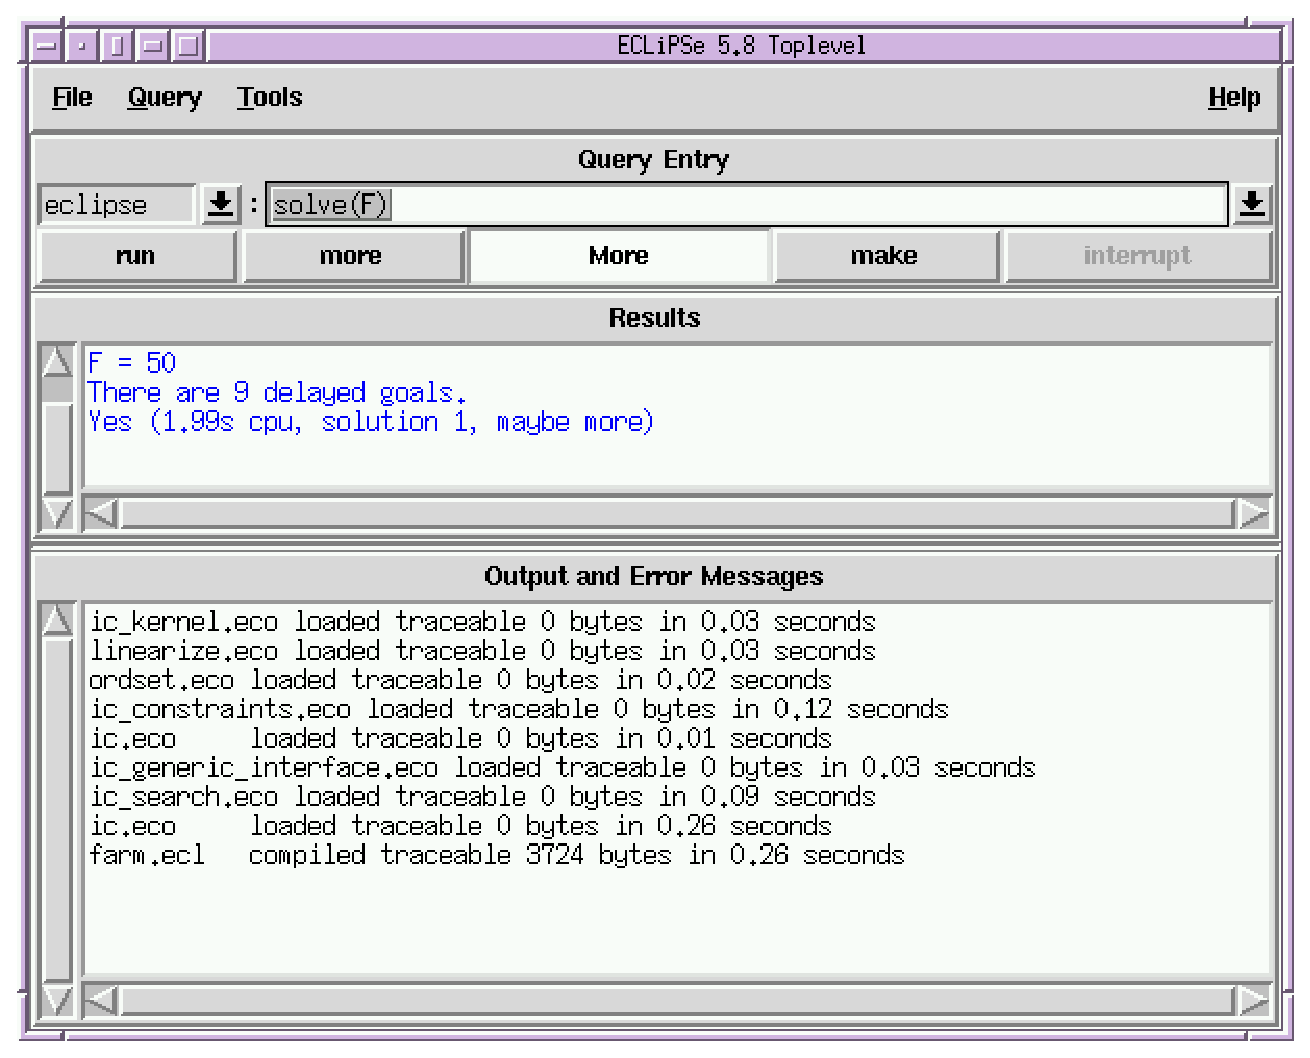
\includegraphics{../userman/tktop.eps}}
\end{center}
\caption{{\tkeclipse} top-level}
\label{tktop}
\end{figure}

Note that help on {\tkeclipse} and its component tools is available
from the \menu{Help} menu in the top-level window.

%------------------------------------------------------------------------
\section{How do I write an {\eclipse} program?}
%------------------------------------------------------------------------
You need to use an editor to write your programs. {\eclipse} does not come
with an editor, but any editor that can save plain text files can be used. 
Save your program as a plain text file, and you can then compile the
program into {\eclipse} and run it.

Extra support for editing {\eclipse} programs with common editors are
available. An eclipse mode for the GNU emacs editor is bundled with the
{\eclipse} package. This mode provides syntax highlighting, automatic
indentation and many other features. To use this mode, you need to load the
\texttt{eclipse.el} file into emacs. This is done by adding the following
line to your \texttt{.emacs} file:

\begin{small}
\begin{verbatim}
(autoload 'eclipse-mode "<eclipsedir>/lib_public/eclipse.el" "ECLIPSE editing mode" t)
\end{verbatim}
\end{small}

where \texttt{<eclipsedir>} is the path to your {\eclipse} installation
directory. 
 
With {\tkeclipse}, you can specify the editor you want to use, and this
editor will be started by {\tkeclipse}, e.g. when you select a file in
the `Edit' option under the File menu. The default values are the value of
the VISUAL environment variable  under Unix, or Wordpad under Windows.
This can be changed with the Preference Editor under the Tools menu.

%------------------------------------------------------------------------
\subsection{Compiling a program}

\index{compile}
From the \menu{File} menu, select the \menuopt{Compile ...} option.
This will bring up a file selection dialogue.  Select the file you wish
to compile, and click on the \button{Open} button.  This will compile
the file and any others it depends on.  Messages indicating which
files have been compiled and describing any errors encountered will be
displayed in the bottom portion of the {\tkeclipse} window
(\guitext{Output and Error Messages}).

If a file has been modified since it was compiled, it may be
recompiled by clicking on the \guitext{make} button.  This recompiles
any files which have become out-of-date.

\See{For more information on program compilation and the compiler,
please see \textbf{The Compiler} chapter in the user manual.}

%------------------------------------------------------------------------
\subsection{Executing a query}

\index{query}
To execute a query, first enter it into the \guitext{Query Entry} text
field.  You will also need to specify which module the query should be
run from, by selecting the appropriate entry from the drop-down list
to the left of the \guitext{Query Entry} field.  Normally, the default
selection of \guitext{eclipse} will be fine; this will allow access to
all {\eclipse} built-ins and all predicates that have not explicitly
been compiled into a different module.  Selecting another module for
the query is only needed if you wish to call a predicate which is not
visible from the {\tt eclipse} module, in which case you need to
select that module.  \See{For more information about the module
system, please see the \textbf{Module System} chapter in the user
manual.}

To actually execute the query, either hit the \keyboard{Enter} key
while editing the query, or click on the \guitext{run} button.
{\tkeclipse} maintains a history of commands entered during the
session, and these may be recalled either by using the drop-down list
to the right of the \guitext{Query Entry} field, or by using the up
and down arrow keys while editing the \guitext{Query Entry} field.

If {\eclipse} cannot find a solution to the query, it will print
\texttt{No} in the \guitext{Results} section of the {\tkeclipse}
window.  If it finds a solution and knows there are no more, it will
print it in the \guitext{Results} section, and then print
\texttt{Yes}.  If it finds a solution and there may be more, it will
print the solution found as before, print \texttt{More}, and enable
the \guitext{more} button.  Clicking on the \guitext{more} button
tells {\eclipse} to try to find another solution.  In all cases it
also prints the total time taken to execute the query.

From \menu{Query} menu, you can run the query with various analysis tools
(see chapter~\ref{sec:program-analysis}): \menuopt{Time Profile} option
will run the query with the profiler tool; \menuopt{Port Profile} option
will run the query with the port profiler tool. 

Note that a query can be interrupted during execution by clicking on
the \guitext{interrupt} button.

%------------------------------------------------------------------------
\subsection{Editing a file}
\label{secedit}

If you wish to edit a file (e.g. a program source file), then you may
do so by selecting the \guitext{Edit ...} option from the
\guitext{File} menu (or use the \guitext{Edit new ...} option if the file
does not yet exist).  This will bring up a file selection dialogue.
Select the file you wish to edit, and click on the \guitext{Open}
button.

When you have finished editing the file, save it.  After you've saved
it, if you wish to update the version compiled into {\eclipse}
(assuming it had been compiled previously), simply click on the
\guitext{make} button.

You can change which program is used to edit your file by using the
{\tkeclipse} Preference Editor, available from the \guitext{Tools}
menu.  Alternatively you can use your editor separately from
\eclipse{}.

%------------------------------------------------------------------------
\subsection{Debugging a program}
\label{secdebug}

To help diagnose problems in {\eclipse} programs, {\tkeclipse}
provides the tracer.  It is activated by selecting the
\guitext{Tracer} option from the \guitext{Tools} menu.  The next time
a goal is executed, the tracer window will become active, allowing you
to step through the program's execution and examine the program's
state as it executes.  A full example is given in
chapter~\ref{chapdebug}.

%------------------------------------------------------------------------
\subsection{File menu}

The \guitext{File} menu of {\tkeclipse} provides various options to
manipulate files:

\subsubsection{Compile} 
Allows the user to select a file to compile into {\eclipse}. 

\subsubsection{Use module}
Allows the user to select and load an {\eclipse} module file into
{\eclipse}.

\subsubsection{Edit} 
Allows the user to select a file to edit using the default text editor 
\See{See section~\ref{secedit} for more information on editors.}.

\subsubsection{Edit new}
Allows the user to specify a new file that will be opened with the default
text editor.

\subsubsection{Cross referencer}
Allows the user to select an {\eclipse} source file and produce a cross
reference over it, and display the resulting graph in a new window.

\subsubsection{Change directory}
Allows the user to change the current working directory.

\subsubsection{Change to example directory}
Change the current working directory to the example directory in the
{\eclipse} distribution.

\subsubsection{New module}
Allows the user to specify a new module that will be created.  The new
module becomes the current toplevel module.  


\subsubsection{Clear toplevel module} 
Allows the user to clear the current toplevel module, i.e. to erase it and
start with a fresh, empty module.

\subsubsection{Exit}
 Leave {\eclipse}


%------------------------------------------------------------------------
\subsection{Getting help}

\index{help}
More detailed help than is provided here can be obtained online for
all the features of {\tkeclipse}.  Simply select the entry from the
\guitext{Help} menu on {\tkeclipse}'s top-level window which
corresponds to the topic or tool you are interested in.

Detailed documentation about all the predicates in the
{\eclipse} libraries can be obtained through the
\guitext{Library Browser and Help} tool.
This tool allows you to browse the online help for the {\eclipse}
libraries.  On the left is a tree display of the libraries available
and the predicates they provide.
\begin{itemize}
\item Double clicking on a node in this tree either expands it or
collapses it again.
\item Clicking on an entry displays help for that entry to the right.
\item Double clicking on a word in the right-hand pane searches for
help entries containing that string.
\end{itemize}
You can also enter a search string or a predicate specification
manually in the text entry box at the top right.  If there is only one
match, detailed help for that predicate is displayed.  If there are
multiple matches, only very brief help is displayed for each; to get
detailed help, try specifying the module and/or the arity of the
predicate in the text field.

Alternatively, you can call the help/1 predicate in the query window
(which contains the same information as the HTML Reference Manual).
It has two modes of operation.  First, when a fragment of a built-in
name is specified, a list of short descriptions of all built-ins whose
name contains the specified string is printed.  For example,
\begin{quote}
\begin{verbatim}
?- help(write).
\end{verbatim}
\end{quote}
will print one-line descriptions about {\bf \tt write/1}, {\bf \tt
writeclause/2}, etc.  When a unique specification is given, the full
description of the specified built-in is displayed, e.g.\ in
\begin{quote}
\begin{verbatim}
?- help(write/1).
\end{verbatim}
\end{quote}
or
\begin{quote}
\begin{verbatim}
?- help(ic:alldifferent/1).
\end{verbatim}
\end{quote}


%------------------------------------------------------------------------
\subsection{Other tools}

{\tkeclipse} comes with a number of useful tools.  Some have been
mentioned above, but here is a more complete list.  Note that we only
provide brief descriptions here; for more details, please see the
online help for the tool in question.

\subsubsection{Compile scratch-pad}

This tool allows you to enter small amounts of program code and have
it compiled.  This is useful for quick experimentation, but not for
larger examples or programs you wish to keep, since the source code is
lost when the session is exited.

\subsubsection{Source File Manager}

This tool allows you to keep track of and manage which source files
have been compiled in the current {\eclipse} session.  You can select
files to edit them, or compile them individually, as well as adding
new files.

\subsubsection{Predicate Browser}

This tool allows you to browse through the modules and predicates
which have been compiled in the current session.  It also lets you
alter some properties of compiled predicates.

\subsubsection{Source Viewer}

This tool attempts to display the source code for predicates selected
in other tools.

\subsubsection{Delayed Goals}

This tool displays the current delayed goals, as well as allowing a
spy point to be placed on the predicate and the source code viewed.

\subsubsection{Inspector}

This tool provides a graphical browser for inspecting terms.  Goals
and data terms are displayed as a tree structure.  Sub-trees can be
collapsed and expanded by double-clicking.  A navigation panel can be
launched which provides arrow buttons as an alternative way to
navigate the tree.

Note that while the inspector window is open, interaction with other
{\tkeclipse} windows is disallowed.  This prevents the term from
changing while being inspected.  To continue {\tkeclipse}, the
inspector window must be closed.

\subsubsection{Visualisation Client}

This starts a new Java visualisation client that allows {\eclipse} programs
to be visualised with the visualisation tools. See the Visualisation manual
for details on the visualisation tools.

\subsubsection{Global Settings}

This tool allows the setting of some global flags governing the way
{\eclipse} behaves.  See also the documentation for the
\bipref{set_flag/2}{../bips/kernel/env/set_flag-2.html} and
\bipref{get_flag/2}{../bips/kernel/env/get_flag-2.html} predicates.

\subsubsection{Statistics}

This tool displays some statistics about memory and CPU usage of the
{\eclipse} system, updated at regular intervals.  See also the
documentation for the
\bipref{statistics/0}{../bips/kernel/env/statistics-0.html} and
\bipref{statistics/2}{../bips/kernel/env/statistics-2.html}
predicates.

\subsubsection{Preference Editor}

This tool allows you to edit and set various user preferences. This
include parameters for how {\tkeclipse} will start up, e.g. the amount
of memory it will be able to use, and a initial query to execute; and
parameters which affects the appearance of {\tkeclipse}, such as the
fonts {\tkeclipse} uses and which editor it launches.


%------------------------------------------------------------------------
\section{How do I make things happen at compile time?}
%------------------------------------------------------------------------

A file being compiled may contain queries.  These are goals
\index{query} preceded by either the symbol ``?-'' or the symbol
``:-''.  As soon as a query or command is encountered in the
compilation of a file, the {\eclipse} system will try to satisfy it.
Thus by inserting goals in this fashion, things can be made to happen
at compile time.

In particular, a file can contain a directive to the system to compile
another file, and so large programs can be split between files, while
still only requiring a single simple command to compile them.
\index{compilation!nesting compile commands} When this happens,
{\eclipse} interprets the pathnames of the nested compiled files
relative to the directory of the parent compiled file; if, for
example, the user calls
\begin{quote}
\begin{verbatim}
[eclipse 1]: compile('src/pl/prog').
\end{verbatim}
\end{quote}
and the file src/pl/prog.pl contains a query
\begin{quote}
\begin{verbatim}
:- [part1, part2].
\end{verbatim}
\end{quote}
then the system searches for the files {\tt part1.pl} and {\tt
part2.pl} in the directory {\tt src/pl} and not in the current
directory.  Usually larger {\eclipse} programs have one main file
which contains only commands to compile all the subfiles.  In
{\eclipse} it is possible to compile this main file from any
directory.  (Note that if your program is large enough to warrant
breaking into multiple files (let alone multiple directories), it is
probably worth turning the constituent components into modules.)
\See{See section~\ref{secmodules} for more information about modules.}

%------------------------------------------------------------------------
\section{How do I use {\eclipse} libraries in my programs?}
\index{libraries}
%------------------------------------------------------------------------

A number of files containing library predicates are supplied with the
{\eclipse} system.  They are usually installed in an {\eclipse}
library directory.  These predicates are either loaded automatically
by {\eclipse} or may be loaded ``by hand''.

During the execution of an {\eclipse} program, the system may
dynamically load files containing library predicates. When this
happens, the user is informed by a compilation or loading message.  It
is possible to explicitly force this loading to occur by use of the
\bipref{lib/1}{../bips/kernel/compiler/lib-1.html} or
\bipref{use_module/1}{../bips/kernel/modules/use_module-1.html}
predicates.  E.g.\ to load the library called {\tt lists}, use one of
the following goals:
\begin{quote}
\begin{verbatim}
:- lib(lists)
:- use_module(library(lists))
\end{verbatim} 
\end{quote}
This will load the library file unless it has been already loaded.  In
particular, a program can ensure that a given library is loaded when
it is compiled, by including an appropriate directive in the source,
e.g.\ {\tt :- lib(lists).}


%------------------------------------------------------------------------
\section{Other tips}
%------------------------------------------------------------------------
\subsection{Recommended file names}

It is recommended programming practice to give the Prolog source
programs the suffix {\bf .pl}, or {\bf .ecl} if it contains {\eclipse}
specific code.  It is not enforced by the system, but it simplifies
managing the source programs.  The
\bipref{compile/1}{../bips/kernel/compiler/compile-1.html} predicate
automatically adds the suffix to the filename, so that it does not
need to be specified; if the literal filename can not be found, the
system tries appending each of the valid suffixes in turn and tries to
find the resulting filename.


%HEVEA\cutend

%% BEGIN LICENSE BLOCK
% Version: CMPL 1.1
%
% The contents of this file are subject to the Cisco-style Mozilla Public
% License Version 1.1 (the "License"); you may not use this file except
% in compliance with the License.  You may obtain a copy of the License
% at www.eclipse-clp.org/license.
% 
% Software distributed under the License is distributed on an "AS IS"
% basis, WITHOUT WARRANTY OF ANY KIND, either express or implied.  See
% the License for the specific language governing rights and limitations
% under the License. 
% 
% The Original Code is  The ECLiPSe Constraint Logic Programming System. 
% The Initial Developer of the Original Code is  Cisco Systems, Inc. 
% Portions created by the Initial Developer are
% Copyright (C) 2006 Cisco Systems, Inc.  All Rights Reserved.
% 
% Contributor(s): 
% 
% END LICENSE BLOCK

\chapter{Prolog Introduction}
%HEVEA\cutdef[1]{section}


\section{Terms and their data types}
\index{term} \index{types}
Prolog data ({\bf terms}) and programs are built from a small set of
simple data-types.  In this section, we introduce these data types
together with their syntax (their textual representations).  For the
full syntax see the User Manual appendix on Syntax.

%Syntactically, even the program code itself is made from valid
%Prolog data-structures, which makes so-called meta-programming
%(which means to treat programs as data) easy.

%We shall first introduce
%the various data types, and then describe how Prolog programs can be built.


\subsection{Numbers}
\index{types!integer} \index{integer numbers}
\index{number}
Numbers come in several flavours. The ones that are familiar from
other programming languages are integers and floating point numbers.
Integers in {\eclipse} can be as large as fits into the machine's
memory:
\begin{quote}\begin{verbatim}
123  0   -27   3492374892749289174
\end{verbatim}\end{quote}
\index{types!float} \index{floating point numbers}
Floating point numbers (represented as IEEE double floats) are written
as
\begin{quote}\begin{verbatim}
0.0 3.141592653589793 6.02e23 -35e-12 -1.0Inf
\end{verbatim}\end{quote}
\index{types!rational} \index{rational numbers} \index{types!bounded
real} \index{bounded reals}
{\eclipse} provides two additional numeric types, rationals and
bounded reals.  {\eclipse} can do arithmetic with all these numeric
types.

Note that performing arithmetic requires the use of the \index{is/2}
\bipref{is/2}{../bips/kernel/arithmetic/is-2.html} predicate:

\begin{quote}\begin{verbatim}
?- X is 3 + 4.
X = 7
Yes
\end{verbatim}\end{quote}

\index{=/2}
If one just uses \bipref{=/2}{../bips/kernel/termcomp/E-2.html},
\eclipse{} will simply construct a term corresponding to the
arithmetic expression, and will not evaluate it:

\begin{quote}\begin{verbatim}
?- X = 3 + 4.
X = 3 + 4
Yes
\end{verbatim}\end{quote}

\See{For more details on numeric types and arithmetic in general see the
User Manual chapter on Arithmetic.}

\See{For more information on the bounded real numeric type, see
Chapter~\ref{chapreal}.}

%Rational numbers implement the corresponding mathematical
%notion, i.e.\ the ratio of two integers, and are written like
%\begin{quote}\begin{verbatim}
%1_3  -30517578125_32768  0_1
%\end{verbatim}\end{quote}
%Bounded reals are a representation for a real number that lies between
%two floating-point bounds, e.g.
%\begin{quote}\begin{verbatim}
%3.141592653__3.141592654
%\end{verbatim}\end{quote}
%{\eclipse} can do arithmetic with all these numeric types.
%For more details see the User Manual chapter on Arithmetic.


\subsection{Strings}

\index{string} \index{types!string}
Strings are a representation for arbitrary sequences of bytes and are
written with double quotes:
\begin{quote}\begin{verbatim}
"hello"
"I am a string!"
"string with a newline \n and a null \000 character"
\end{verbatim}\end{quote}
Strings can be constructed and partitioned in various ways using
{\eclipse} primitives.


\subsection{Atoms}

\index{atom} \index{types!atom}
Atoms are simple symbolic constants, similar to enumeration type
constants in other languages. No special meaning is attached to them
by the language.  Syntactically, all words starting with a lower case
letter are atoms, sequences of symbols are atoms, and anything in
single quotes is an atom:
\begin{quote}\begin{verbatim}
atom  quark  i486  -*-  ???  'Atom'   'an atom'
\end{verbatim}\end{quote}


\subsection{Lists}

\index{list} \index{types!list}
A list is an ordered sequence of (any number of) elements, each of
which is itself a term. Lists are delimited by square brackets ({\tt [
]}), and elements are separated by a comma. Thus, the following are
lists:
\begin{quote}\begin{verbatim}
[1,2,3]
[london, cardiff, edinburgh, belfast]
["hello", 23, [1,2,3], london]
\end{verbatim}\end{quote}
\index{empty list} \index{nil@\textit{nil}}
A special case is the empty list (sometimes called {\em nil}), which
is written as
\begin{quote}\begin{verbatim}
[]
\end{verbatim}\end{quote}
A list is actually composed of head-and-tail pairs, where the head contains one
list element, and the tail is itself a list (possibly the empty list).
Lists can be written as a {\tt [Head|Tail]} pair, with the head separated from
the tail by the vertical bar. Thus the list {\tt [1,2,3]} can
be written in any of the following equivalent ways:
\begin{quote}\begin{verbatim}
[1,2,3]
[1|[2,3]]
[1|[2|[3]]]
[1|[2|[3|[]]]]
\end{verbatim}\end{quote}
The last line shows that the list actually consists of 3 {\tt [Head|Tail]}
pairs, where the tail of the last pair is the empty list.
The usefulness of this notation is
that the tail can be a variable (introduced below):
{\tt [1|Tail]}, which leaves the tail unspecified for the moment. 


\subsection{Structures} 

\index{structure} \index{types!structures}
Structures correspond to structs or records in other languages.  A
structure is an aggregate of a fixed number of components, called its
{\em arguments}. Each argument is itself a term.  Moreover, a
structure always has a name (which looks like an atom).  The canonical
syntax for structures is
\begin{quotation}
{\it $<$name$>$($<$arg$>_{1}$,...$<$arg$>_{n}$)}
\end{quotation}
Valid examples of structures are:
\begin{quote}\begin{verbatim}
date(december, 25, "Christmas")
element(hydrogen, composition(1,0))
flight(london, new_york, 12.05, 17.55)
\end{verbatim}\end{quote}
\index{arity} The number of arguments of a structure is called its {\em
arity}.  \index{functor} The name and arity of a structure are
together called its {\em functor} and is often written as {\em
name/arity}.  The last example above therefore has the functor {\tt
flight/4}.

\See{See section \ref{structures} for information about defining structures
with named fields.}

\subsubsection{Operator Syntax} 
\index{operator syntax}
\index{infix}
\index{prefix}
\index{postfix}
As a syntactic convenience, unary (1-argument) structures can also be written
in prefix or postfix notation, and binary (2-argument) structures can be
written in prefix or infix notation, if the programmer has made an
appropriate declaration (called an {\em operator declaration})
about its functor.  For example if {\tt plus/2} were declared to
be an infix operator, we could write:
\begin{quote}\begin{verbatim}
1 plus 100
\end{verbatim}\end{quote}
instead of
\begin{quote}\begin{verbatim}
plus(1,100)
\end{verbatim}\end{quote}
It is worth keeping in mind that the data term represented by the
two notations is the same, we have just two ways of writing the same thing.
Various logical and arithmetic functors are automatically declared to
allow operator syntax, for example {\tt +/2, not/1} etc.

\subsubsection{Parentheses} 
When prefix, infix and postfix notation is used, it is sometimes necessary to
write extra parentheses to make clear what the structure of the written
term is meant to be. For example to write the following nested structure
\begin{quote}\begin{verbatim}
+(*(3,4), 5)
\end{verbatim}\end{quote}
we can alternatively write
\begin{quote}\begin{verbatim}
3 * 4 + 5
\end{verbatim}\end{quote}
because the star binds stronger than the plus sign.
But to write the following differently nested structure
\begin{quote}\begin{verbatim}
*(3, +(4, 5))
\end{verbatim}\end{quote}
in infix-notation, we need extra parentheses:
\begin{quote}\begin{verbatim}
3 * (4 + 5)
\end{verbatim}\end{quote}
A full table of the predefined prefix, infix and postfix operators
with their relative precedences can be found in the appendix of the
User Manual.

\quickref{Summary of Data Types}{
\begin{description}
\item[Numbers]
        \eclipse has {\em integers}, {\em floats}, {\em rationals} and {\em bounded reals}.
\item[Strings]
        Character sequences in double quotes.
\item[Atoms]
        Symbolic constants, usually lower case or in single quotes.
\item[Lists]
        Lists are constructed from cells that have an arbitrary head and
        a tail which is again a list.
\item[Structures]
        Structures have a name and a certain number ({\em arity}) of arbitrary arguments.
        This characteristic is called the {\em functor}, and written name/arity.
\end{description}
}


\section{Predicates, Goals and Queries}

\index{predicate}
\index{goal}
\index{query}
Where other programming languages have procedures and functions,
Prolog and {\eclipse} have {\em predicates}.  A predicate is something
that has a truth value, so it is similar to a function with a boolean result.
A predicate {\em definition} simply defines what is true.
A predicate {\em invocation} (or {\em call}) checks whether something is true or false.
\index{integer/1}
A simple example is the predicate {\em integer/1}, which has a built-in
definition. It can be called to check whether something is an integer:
\begin{quote}\begin{verbatim}
integer(123)           is true
integer(atom)          is false
integer([1,2])         is false
\end{verbatim}\end{quote}
A predicate call like the above is also called a {\em goal}.
A starting goal that the user of a program provides is called a {\em query}.
To show queries and their results, we will from now on
use the following notation:
\begin{quote}\begin{verbatim}
?- integer(123).
Yes.
?- integer(atom).
No.
?- integer([1,2]).
No.
\end{verbatim}\end{quote}
A query can simply be typed at the eclipse prompt, or entered into the
query field in a tkeclipse window. Note that it is not necessary to enter
the {\tt ?-} prefix.
On a console input, is however necessary to terminate the query with a
full-stop (a dot followed by a newline).
After executing the query, the system will print one of the
answers {\bf Yes} or {\bf No}.


\subsection{Conjunction and Disjunction}
\index{conjunction}
\index{disjunction}

\index{conjunction} \index{disjunction}
Goals can be combined to form conjunctions (AND) or disjunctions (OR).
Because this is so common, Prolog uses the comma for AND and the
semicolon for OR. The following shows two examples of conjunction,
the first one is true because both conjuncts are true, the second is false:
\begin{quote}\begin{verbatim}
?- integer(5), integer(7).
Yes.
?- integer(5), integer(hello).
No.
\end{verbatim}\end{quote}
In contrast, a disjunction is only false if both disjuncts are false:
\begin{quote}\begin{verbatim}
?- ( integer(hello) ; integer(5) ).
Yes.
?- ( integer(hello) ; integer(world) ).
No.
\end{verbatim}\end{quote}
As in this example, it is advisable to always surround disjunctions with
parentheses. While not strictly necessary in this example, they are often
required to clarify the structure.

In practice, when answering queries with disjunctions, the system will
actually give a separate {\bf Yes} answer for every way in which the
query can be satisfied (i.e.\ proven to be true).
For example, the following disjunction can be satisfied in two ways,
therefore system will give two {\bf Yes} answers:
\begin{quote}\begin{verbatim}
?- ( integer(5) ; integer(7) ).
Yes (0.00s cpu, solution 1, maybe more)
Yes (0.02s cpu, solution 2)
\end{verbatim}\end{quote}
The second answer will only be given after the user has explicitely
asked for more solutions.
Sometimes the system cannot decide whether an answer is the last one.
In that case, asking for more solutions may lead to an alternative
{\bf No} answer, like in the following example:
\begin{quote}\begin{verbatim}
?- ( integer(5) ; integer(hello) ).
Yes (0.00s cpu, solution 1, maybe more)
No (0.02s cpu)
\end{verbatim}\end{quote}
Of course, as long as there was at least one {\bf Yes} answer, the query
as a whole was true.


\section{Unification and Logical Variables}

\subsection{Symbolic Equality}
\index{equality!symbolic}
Prolog has a particularly simple idea of {\bf equality}, namely
structural equality by pattern matching.  This means that two terms
are equal if and only if they have exactly the same structure.  No
evaluation of any kind is perfomed on them:
\begin{quote}\begin{verbatim}
?- 3 = 3.
Yes.
?- 3 = 4.
No.
?- hello = hello.
Yes.
?- hello = 3.
No.
?- foo(a,2) = foo(a,2).
Yes.
?- foo(a,2) = foo(b,2).
No.
?- foo(a,2) = foo(a,2,c).
No.
?- foo(3,4) = 7.
No.
?- +(3,4) = 7.
No.
?- 3 + 4 = 7.
No.
\end{verbatim}\end{quote}
Note in particular the last two examples (which are equivalent):
there is no automatic arithmetic evaluation. The term +(3,4) is simply
a data structure with two arguments, and therefore of course different from
any number.

Note also that we have used the built-in predicate =/2, which exactly
implements this idea of equality.


\subsection{Logical Variables}
\index{logical variable}

\index{variables} \index{logical variables}
So far we have only performed tests, giving only Yes/No results.
How can we compute more interesting results? 
The solution is to introduce Logical Variables. 
It is very important to understand that Logical Variables are
variables in the mathematical sense, not in the usual programming
language sense. Logical Variables are simply placeholders for
values which are not yet known, like in mathematics.
In conventional programming languages on the other hand, variables
are labels for storage locations.
The important difference is that the value of a logical variables is
typically unknown at the beginning, and only becomes
known in the course of the computation. Once it is known, the variable is just
an alias for the value, i.e. it refers to a term.
Once a value has been assigned to a logical variable, it remains fixed
and cannot be assigned a different value. 

Logical Variables are written beginning with an upper-case letter or
an underscore, for example
\begin{quote}\begin{verbatim}
X   Var   Quark   _123   R2D2
\end{verbatim}\end{quote}
If the same name occurs repeatedly in the same input term (e.g. the same
query or clause), it denotes the same variable.


\subsection{Unification}
\index{unification}

\index{unification} \index{instantiation} \index{aliasing} \index{binding}
With logical variables, the above equality tests become much more interesting,
resulting in the concept of {\em Unification}.
Unification is an extension of the idea of pattern matching of two terms.
In addition to matching, unification also causes the binding (instantiation,
aliasing) of variables in the two terms.
Unification instantiates variables such that the two unified terms become
equal. For example
\begin{quote}\begin{verbatim}
X = 7                is true with X instantiated to 7
X = Y                is true with X aliased to Y (or vice versa)
foo(X) = foo(7)      is true with X instantiated to 7
foo(X,Y) = foo(3,4)  is true with X instantiated to 3 and Y to 4
foo(X,4) = foo(3,Y)  is true with X instantiated to 3 and Y to 4
foo(X) = foo(Y)      is true with X aliased to Y (or vice versa)
foo(X,X) = foo(3,4)  is false because there is no possible value for X
foo(X,4) = foo(3,X)  is false because there is no possible value for X
\end{verbatim}\end{quote}



\quickref{Basic Terminology}{
\begin{description}
\item[Predicate] Something that is true or false, depending on its definition
    and its arguments. Defines a relationship between its arguments.
\item[Goal] A logical formula whose truth value we want to know.
    A goal can be a conjunction or disjunction of other (sub-)goals.
\item[Query] The initial Goal given to a computation.
\item[Unification] An extension of pattern matching which can bind logical
    variables (placeholders) in the matched terms to make them equal.
\item[Clause] One alternative definition for when a predicate is true.
    A clause is logically an implication rule.
\end{description}
}





\section{Defining Your Own Predicates}

\subsection{Comments}
\index{comment}
       Since we will annotate some of our programs, we first introduce
       the syntax for comments. There are two types:
       \begin{description}
        \item[Block comment] The comment is enclosed between the delimiters {\tt /*} and {\tt */}.
         Such comments can span multiple lines, and may be conveniently used
         to comment out unused code.
       \item[Line comment] Anything following and including '{\tt \%}' in a line is taken as a
       comment (unless 
        the '{\tt \%}' character is part of a quoted atom or string).
       \end{description}

\subsection{Clauses and Predicates}
\label{syntax}
\index{clause}

     \index{clause} \index{predicate}
     Prolog programs are built from valid Prolog data-structures.
     A program is a collection of {\it predicates}, and a
     predicate is a collection of {\it clauses}.

     The idea of a clause is to define that something is true.
     The simplest form of a clause is the {\em fact}.
     For example, the following two are facts:
\begin{code}
capital(london, england).
brother(fred, jane).
\end{code}
     Syntactically, a fact is just a structure (or an atom)
     terminated by a full stop.

     Generally, a clause has the form
     \begin{quote}
     Head :- Body.
     \end{quote}
     where {\em Head} is a structure (or atom) and {\em Body} is a {\em Goal},
     possibly with conjunctions and disjunctions like in the queries discussed above.
     The following is a clause
\begin{code}
uncle(X,Z) :- brother(X,Y), parent(Y,Z).
\end{code}
     Logically, this can be read as a reverse implication
     \begin{quote}
     $uncle(X,Z) \longleftarrow brother(X,Y) \wedge parent(Y,Z)$
     \end{quote}
     or, more precisely
     \begin{quote}
     $\forall X \forall Z: uncle(X,Z) \longleftarrow \exists Y: brother(X,Y) \wedge parent(Y,Z)$
     \end{quote}
     stating that uncle(X,Z) is true if brother(X,Y) and parent(Y,Z) are true.
     Note that a fact is equivalent to a clause where the body is {\tt true}:
\begin{code}
brother(fred, jane) :- true.
\end{code}

     One or multiple clauses with the same head functor (same name and number
     of arguments) together form the {\em definition}
     of a predicate. Logically, multiple clauses are read as a disjunction,
    i.e.\ they define alternative ways in which the predicate can be true.
     The simplest case is a collection of alternative facts:
\begin{code}
parent(abe, homer).
parent(abe, herbert).
parent(homer, bart).
parent(marge, bart).
\end{code}
The following defines the ancestor/2 predicate by giving two alternative
clauses (rules):
\begin{code}
ancestor(X,Y) :- parent(X,Y).
ancestor(X,Y) :- parent(Z,Y), ancestor(X,Z).
\end{code}
       Remember that a clause can be read logically, with the {\tt :-}
       taking the meaning of implication, and the comma
       separating goals read as a conjunction. The logical
       reading for several clauses of the same predicate is disjunction
       between the clauses. So the first
       ancestor rule above states that if X is a parent of Y, then this
       implies that X is an ancestor of Y. The second rule, which specifies
       another way X can be an ancestor of Y states that if some other
       person, Z, is the parent of Y, {\it and\/} X is an ancestor of Z,
       then this implies that X is also an ancestor of Y.

%       In fact, syntactically, the {\tt ':-'} and {\tt ','} used in 
%       constructing clauses are operators ({\tt :-/2} and {\tt ,/2}
%       if a clause contains more than two body goals, this is achieved by
%       nesting of {\tt ,/2}).

\Note{
\index{variables!scope}
It is also important to remember that the scope of a variable
       name only extends over the clause in which it is in, so any
       variables with the same name in the same clause refer to the
       same variable, but variables which occur in different clauses
       are different even if they have been written with the same name.
       }


\section{Execution Scheme}

%       Before we describe the execution of Prolog programs in more detail, we
%       shall first discuss the basic mechanism for computation in Prolog --
%       unification.  
%
%\subsection{Unification}
%
%  Unification is the pattern matching of two terms. In addition to
%  matching, unification also causes the binding (aliasing) of
%  variables in the two terms. For example,
%  \begin{quotation}
%  unifying {\tt capital(london,Country) } with {\tt capital(london,england)} will
%  cause {\tt Country} to bind to 
%  {\tt england}.
%  \end{quotation}
%
%   Note that variables from the two terms being unified can both supply
%   variables that are bound, e.g. unifying
%
%\begin{verbatim}
%   capital(City,england)      capital(london, Country)
%\end{verbatim}
%
%   would bind {\tt City} to {\tt london}, and {\tt Country} to {\tt england}.
%
%   If the two terms being unified do not match with each other, then the 
%   unification {\bf fails}. Here are examples of pairs of terms that fail
%   to unify:
%\begin{verbatim}
%
%       london                    france
%       capital(City,Country)     ancestor(X,Y)
%       capital(london, Country)  capital(paris, Country)
%
%\end{verbatim}
%

\subsection{Resolution}
\index{resolution}

\index{resolution} \index{resolvent}
Resolution is the computation rule used by Prolog. Given a set of
facts and rules as a program, execution begins with a query, which is
an initial goal that is to be resolved.
The set of goals that still have to be resolved is called the
{\em resolvent}.

Consider again the {\tt ancestor/2}
and {\tt parent/2} predicate shown above.
\begin{code}
ancestor(X,Y) :- parent(X,Y).                 % clause 1
ancestor(X,Y) :- parent(Z,Y), ancestor(X,Z).  % clause 2 

parent(abe, homer).                           % clause 3
parent(abe, herbert).                         % clause 4
parent(homer, bart).                          % clause 5
parent(marge, bart).                          % clause 6
\end{code}
Program execution is started by issuing a query, for example
\begin{quote}\begin{verbatim}
?- ancestor(X, bart).
\end{verbatim}\end{quote}
This is our initial resolvent.
The execution mechanism is now as follows:
\exercises{Execution Algorithm}{
\begin{enumerate}
\item Pick one (usually the leftmost) goal from the resolvent.
        If the resolvent is empty, stop.
\item Find all clauses whose head successfully unifies with this goal.
        If there is no such clause, go to step 6.
\item Select the first of these clause. If there are more, remember the
        remaining ones. This is called a {\em choice point}.
\item Unify the goal with the head of the selected clause.
        (this may instantiate variables both in the goal and in the clause's body).
\item Prefix this clause body to the resolvent and go to 1.
\item \index{backtracking}
      Backtrack: Reset the whole computation state to
        how it was when the most recent choice point was created.
        Take the clauses remembered in this choice point and go to 3.
\end{enumerate}
}
In our example, the Prolog system would attempt to unify
{\tt ancestor(X, bart)} with the program's
clause heads. Both clauses of the {\tt ancestor/2} predicate can
unify with the goal, but the textually first clause, clause 1, is
selected first, and successfully unified with the goal:
\begin{quote}\begin{verbatim}
Goal (Query):   ancestor(X,bart)
Selected:       clause 1
Unifying:       ancestor(X,bart) = ancestor(X1,Y1)
results in:     X=X1, Y1=bart
New resolvent:  parent(X, bart)
More choices:   clause 2
\end{verbatim}\end{quote}
The body goal of clause 1 \verb'parent(X, bart)' is added to the
resolvent, and the system remembers that there is an untried 
alternative -- this is referred to as a {\it choice-point}.

In the same way, \verb'parent(X, bart)' is next selected for 
unification. Clauses 5 and 6 are possible matches for this goal,
with clause 5 selected first. There are no body goals to add, and
the resolvent is now empty:
\begin{quote}\begin{verbatim}
Goal:           parent(X, bart)
Selected:       clause 5
Unifying:       parent(X,bart) = parent(homer,bart)
results in:     X = homer
New resolvent:  
More choices:   clause 6, then clause 2
\end{verbatim}\end{quote}
The execution of a program completes successfully when there is an
empty resolvent. The program has thus found the first solution 
to the query, in the form of instantiations to the original Query's
variables, in this case {\tt X = homer}. \eclipse\ returns this
solution, and also asks if we want more solutions:
\begin{quote}\begin{verbatim}
?- ancestor(X,bart).
X = homer     More? (;) 
\end{verbatim}\end{quote}
Responding with ';' will cause \eclipse\ to try to find alternative
solutions by {\bf backtracking} to
the most recent choice-point, i.e. to seek an alternative to 
{\tt parent/2}. Any bindings done during and after the selection of 
clause 5 are undone, i.e. the binding of  X to {\tt 
homer} is undone. Clause 6 is now unified with
the goal {\tt parent(X,Y)}, which again produces a solution:
\begin{quote}\begin{verbatim}
Goal:           parent(X, bart)
Selected:       clause 6
Unifying:       parent(X,bart) = parent(marge,bart)
results in:     X = marge
New resolvent:  
More choices:   clause 2
\end{verbatim}\end{quote}
If yet further solutions are needed, then \eclipse\ would again backtrack.
This time, {\tt parent/2} no longer has any alternatives left to unify,
so the next older choice-point, the one made for {\tt ancestor/2},
is the one that would be considered. The computation is returned
to the state it was in just before clause 1 was selected, and clause 2
is unified with the query goal:
\begin{quote}\begin{verbatim}
Goal:           ancestor(X,bart)
Selected:       clause 2
Unifying:       ancestor(X,bart) = ancestor(X1,Y1)
results in:     Y1 = bart, X1 = X
New resolvent:  parent(Z1, bart), ancestor(X1, Z1)
More choices:   
\end{verbatim}\end{quote}
For the first time, there are more than one goal in the resolvent, the
leftmost one, {\tt parent(Z1,bart)} is then
selected for unification. Again, clauses 5 and 6 are candidates, and
a new choice-point is created, and clause 5 tried first.
\begin{quote}\begin{verbatim}
Goal:           parent(Z1, bart)
Selected:       clause 5
Unifying:       parent(Z1, bart) = parent(homer, bart)
results in:     Z1 = homer
New resolvent:  ancestor(X1, homer)
More choices:   clause 6
\end{verbatim}\end{quote}
Eventually, after a few more steps
(via finding the ancestor of {\tt homer}), this leads to a new solution, 
with {\tt abe} returned as an ancestor of {\tt bart}:
\begin{quote}\begin{verbatim}
?- ancestor(X,bart).
X = abe     More? (;) 
\end{verbatim}\end{quote}
If yet more solutions are requested, then because only one parent for
{\tt homer} is given by the program, \eclipse\ would backtrack to the only 
remaining choice-point, unifying clause 6 is unified with the goal, 
binding \verb'Z1' to \verb'marge'. However, no ancestor for {\tt marge}
can be found, because no parent of
{\tt marge} is specified in the program. No more choice-points remains to
be tried, so the execution terminates.



\section{Partial data structures}
\label{tail}
\index{tail}
Logical variables can occur anywhere, not only as arguments of clause
heads and goals, but also within data structures.
A data structure which contains variables is called a partial data
structure, because it will eventually be completed by substituting
the variable with an actual data term.
The most common case of a partial data structure is a list whose
tail is not yet instantiated.

Consider first an example where no partial lists occur.
In the following query, a list is built incrementally,
starting from its end:
\begin{quote}\begin{verbatim}
?- L1 = [], L2 = [c|L1], L3 = [b|L2], L4 = [a|L3].
L1 = []
L2 = [c]
L3 = [b, c]
L4 = [a, b, c]
\end{verbatim}\end{quote}
Whenever a new head/tail cell is created,
the tail is already instantiated to a complete list.

But it is also possible to build the list from the front.
The following code, in which the goals have been reordered,
gives the same final result as the code above:
\begin{quote}\begin{verbatim}
?- L4 = [a|L3], L3 = [b|L2], L2 = [c|L1], L1 = [].
L1 = []
L2 = [c]
L3 = [b, c]
L4 = [a, b, c]
\end{verbatim}\end{quote}
However, in the course of the computation, variables get instantiated to
''partial lists'', i.e.\ lists whose head is known, but whose tail is not.
This is perfectly legal: due to the nature of the logical variable, the
tail can be filled in later by instantiating the variable.

%Partial data structures are in fact a very 
%important feature of Prolog. Variables can occur anywhere inside
%a data structure, and this allows data to be built incrementally and dynamically:
% the partially built data structure is passed
%around, and its ``holes'' (the variables) are filled in by further partial
%data structures.

%THIS IS NOT AN EXAMPLE OF PARTIAL DATA STRUCTURES!
%An example use of partial data structure is in the use of accumulator pairs,
%which was demonstrated in section~\ref{tail} with numbers. However, the
%`value' being accumulated can be a partial data structure, as shown with
%this example of reversing a list:
%\begin{code}
%reverse(List,Reverse) :- rev(List, [], Reverse).
%
%rev([], R, R).
%rev([E|L], R0, R) :- rev(L, [E|R0], R).
%\end{code}
%
%The partially reversed list is being constructed in the second argument of
%\verb'rev/3', and finally passed out when the end of the list is reached.


%\subsection{Difference Lists}
%An important technique using partial data structure is the difference list.
%In difference lists, a list is represented by a pair of (perhaps partial)
%lists, e.g.
%the list \verb'[1,2,3|T]' can be represented as the pair \verb'[1,2,3|T]' and
%\verb'T'. This gives direct access to the tail of a list, and the list does
%not need to be traversed to reach the tail. This can result in much improved
%efficiency when, for example, appending two lists together. With a normal
%list representation, the {\tt append} predicate is written as:
%\begin{code}
%% append(L1, L2, L) L is the list L2 appended to the end of L1
%append([], L, L).
%append([E|L1], L2, [E|L]) :-
%    append(L1, L2, L).
%\end{code}
%
%With this encoding, the first list has to be traversed fully to find
%the end, and then the 
%second list appended to that.
%
%With the difference list representation, the end of the lists are known,
%and the append can be encoded with a simple fact:
%\begin{code}
%/* append_dl(L1,E1, L2,E2, L,E) 
%   L,E is the appended list of L1,E1 and L2,E2 
%*/
%append_dl(L1,E1, E1,E2, L1,E2).
%\end{code}
%
%\begin{figure}
%%\epsfbox{appenddiff.ps}
%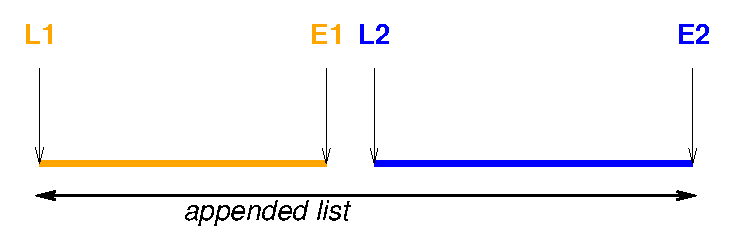
\includegraphics{appenddiff.ps}
%\caption{Appending difference lists}
%\end{figure}
%The situation is as shown in the figure. By setting E1 to L2, the second 
%list is appended to the end of the first list, and \verb'L1',\verb'E2' now
%represents the combined list. With this difference list representation,
%no traversal of the first list is needed, and the operation is done in
%constant time. It can thus be much more efficient, especially if the first
%list is long.

\section{More control structures}
    \subsection{Disjunction}
\index{disjunction} \index{;/2}
Disjunction is normally specified in Prolog by different clauses of
a predicate, but it can also be specified within a single clause by
the use of \verb';/2'. For example,

\begin{code}
atomic_particle(X) :- (X = proton ; X = neutron ; X = electron).
\end{code}

This is logically equivalent to: 

\begin{code}
atomic_particle(proton).
atomic_particle(neutron).
atomic_particle(electron).
\end{code}

    \subsection{Conditional}

\index{conditional} \index{->/2}
Conditionals can be specified using the \verb'->/2' operator.
In combination with \verb';/2', a conditional similar to `if-then-else' 
constructs of conventional language can be constructed:
\verb'X->Y;Z', where \verb'X', \verb'Y' and \verb'Z' can be one or more
goals,  means that if \verb'X' is true, then \verb'Y' will be
executed, otherwise \verb'Z'. Only the first solution of \verb'X' is
explored, so that on backtracking, no new solutions for \verb'X' will be
tried. In addition, if \verb'X' succeeds, then the `else' part, \verb'Z'
will never be tried. If \verb'X' fails, then the `then' part, \verb'Y',
will never be tried. An example of `if-then-else' is:
\begin{code}
max(X,Y, Max) :- 
   number(X), number(Y),
   (X > Y -> Max = X ; Max = Y).
\end{code}
where \verb'Max' is the bigger of the numbers \verb'X' or \verb'Y'.
Note the use of the brackets to make the scope of the if-then-else
clear and correct.


    \subsection{Call} 
\index{call}
\index{metacall}
One feature of Prolog is the equivalence of  programs and data -- both are
represented as terms. The predicate \verb'call' allows 
program terms (i.e. data) to be treated as goals: \verb'call(X)' will cause
\verb'X' to be treated as a goal and executed. Although at the time when 
the predicate is executed, \verb'X' has to be instantiated, it does not 
need to be instantiated (or even known) at compile time. For example, it
would in principle be
possible to define disjunction (\verb';') as follows:

\begin{code}
X ; Y :- call(X).
X ; Y :- call(Y).
\end{code}

%In addition, a Prolog program can construct a term at run-time, which is then 
%called as a goal.  This is sometimes used to ensure goals are compiled
%after earlier goals have already been executed, for
%example\footnote{The 'foreach' construct is described in the next chapter.}:
%\begin{verbatim}
%Y=A, call(foreach(A,[a,b,c]) do writeln(Y)).
%\end{verbatim}
%As required, this means the same as
%\begin{verbatim}
%foreach(A,[a,b,c]) do writeln(A).
%\end{verbatim}


\subsection{All Solutions}
\label{all-solutions}

In the pure computational model of Prolog, alternative solutions are
computed one-by-one on backtracking. Only one solution is available
at any time, while previous solutions disappear on backtracking:
\begin{quote}\begin{verbatim}
?- weekday(X).
X = mo
More
X = tu
More
X = we
More
...
\end{verbatim}\end{quote}
Sometimes it is useful to have all solution together in a list.
This can be achieved by using one of the all-solutions predicates
\index{findall/3}\index{setof/3}\index{bagof/3}findall/3, setof/3 or bagof/3:
\begin{quote}\begin{verbatim}
?- findall(X, weekday(X), List).
X = X
List = [mo, tu, we, th, fr, sa, su]
Yes
\end{verbatim}\end{quote}
\See{For the differences between findall/3, setof/3 and bagof/3
see the \eclipse{} Reference Manual.}


\section{Using Cut}
\label{cut}
\index{cut}
Cut (written as \verb'!') prunes away part of the Prolog search-space. This
can be a very powerful mechanism for improving the performance of programs,
and even the suppression of unwanted solutions. However, it can also be
easily misused and over-used. 

Cut does two things:

\begin{description}
\item[commit] Disregard any later clauses for the predicate.
\item[prune] Throw away all alternative solutions to the goals to the left of
 the cut.
\end{description}

\subsection{Commit to current clause}
\index{commit}

Consider the following encoding of the ``minimum'' predicate:
\begin{code}
min(X,Y, Min) :- X <Y, Min = X.
min(X,Y, Min) :- Y=<X, Min = Y.
\end{code}
Whilst logically correct, the behaviour of this encoding is
non-optimal for two reasons.  Consider the goal {\tt :- min(2,3,M)}.
Although the first clause succeeds, correctly instantiating $M$ to
$2$, Prolog leaves an open choice point.  If these clauses and goal
occur as part of a larger program and goal, a failure might occur
later, causing backtracking to this open choice point. 
Prolog would then, in vain, try to find another minimum using the
second clause for {\tt min}.  So there is a double drawback:
firstly, an open choice point consumes memory, and secondly the
unsuccessful evaluation of the second clause costs execution time.

To achieve the same logic, but more efficient behaviour, the
programmer can introduce a {\it cut}.
For example {\tt min} is typically encoded as follows:
\begin{code}
min(X,Y, Min) :- X<Y, !, Min = X.
min(X,Y, Y).
\end{code}
The cut removes the unnecessary choice point, which means that the
second clause will never be executed if the first clause passed the
cut.  This effectively makes the test in the second clause redundant,
and it can therefore be removed.

  \subsection{Prune alternative solutions}
\index{prune}
A cut may occur anywhere where a goal may occur, consider the following:
\begin{code}
first_prime(X, P) :-
    prime(X,P), !.
\end{code}
where \verb'first_prime' returns the first prime number smaller than \verb'X'.
In this case, it calls a predicate \verb'prime/2', which generates prime
numbers smaller than \verb'X', starting from the largest one. The effect of
the cut here is to prune away all the remaining solutions to \verb'prime(X,P)'
once the first one is generated, so that on backtracking, \verb'prime(X,P)'
is not tried for alternative solutions. The cut will also commit the execution
to this clause for \verb'first_prime/2', but as there is only one clause,
this has no visible effect.


%%----------------------------------------------------------------------
%\section{Prolog vs Imperative Languages}
%%----------------------------------------------------------------------
%\quickref{Comparison Prolog vs Imperative Programming}{
%\begin{tabular}{p{7cm}p{7cm}}
%{\bf Prolog} & {\bf Imperative Language} \\
%\hline
%\hline
%set of clauses & program \\
%\hline
%predicate (set of clauses with same name and arity) & procedure \\
%\hline
%clause (rule or fact) & if statement / one arm of nondeterministic case
%        statement / sequence of procedure calls \\
%\hline
%goal invocation & procedure call \\
%\hline
%unification & parameter passing / assignment / dynamic memory allocation /
%        conditional branching \\
%\hline
%backtracking & continuation passing / exception handling /
%        execution state manipulation \\
%\hline
%logical variable & pointer manipulation \\
%\hline
%tail recursion & iteration \\
%\end{tabular}
%}

%----------------------------------------------------------------------
\section{Common Pitfalls}
%----------------------------------------------------------------------
Prolog is different from conventional programming languages, and a common
problem is to program Prolog like a conventional language. Here are some
points to note:

\begin{itemize}
\item Unification is more powerful than normal case discrimination (see 
  section~\ref{unif}); 
\item Prolog procedure calls are more powerful than conventional procedure
calls. In particular, backtracking is possible (see section~\ref{back});
\end{itemize}

    \subsection{Unification works both ways}
\label{unif}
One common problem is to write a predicate expecting certain instantiation
patterns for the arguments, and then get unexpected results when the 
arguments do not conform to the expected pattern. An example is the
member relation, intended to check if an item \verb'Item' is a member of
a list or not. This might be written as:


\begin{code}
member(Item, [Item|_]).
member(Item, [_|List]) :- member(Item, List).
\end{code}

The expected usage assumes both \verb'Item' and the list are ground. In 
such cases, the above predicate does indeed check if \verb'Item' occurs in
the list given as a second argument. However, if either of the arguments are
not ground, then potentially unexpected behaviour might occur. Consider
the case where \verb'Item' is a variable, then the above predicate will 
enumerate the elements of the list successively through backtracking. On
the other hand, if any of the list elements of the list is a variable, they
would be unified with \verb'Item'. Other instantiation patterns for either
arguments can produce even more complex results. 

If the intended meaning is simply to check if \verb'Item' is a member of 
a list, this can be done by:

\begin{code}
  \% is_member(+Element, +List)
  \% check if Element is an element that occurs in a List of
  \% ground elements
is_member(Item, [Element|_]) :- Item == Element.
is_member(Item, [_|List]) :- nonvar(List), is_member(Item, List).
\end{code}

Note the use of comments to make clear the intention of the use of the
predicate. The convention used is that `+' indicates that an argument should
be instantiated (i.e. not a variable), `-' for an argument that should be
an uninstantiated variable, and '?' indicates that there is no restrictions
on the mode of the argument.

    \subsection{Unexpected backtracking}
\label{back}
Remember that when coding in Prolog, any predicate {\it may\/} be backtracked 
into. So correctness in Prolog requires:

\begin{itemize}
\item Predicate returns the correct answer when first called.
\item Predicate behaves correctly when backtracked into.
\end{itemize}

Recall that backtracking causes alternative choices to be explored, if
there are any.  Typically another choice corresponds to another clause
in the poredicate definition, but alternative choices may come from
disjunction (see above) or built-in predicates with multiple
(alternative) solutions. 
The programmer should make sure that a predicate will only produce
those solutions that are wanted. Excess alternatives can be removed by
coding the program not to produce them, or by the cut, or the conditional.

For example, to return only the {\it first\/} member, in the
\verb'is_member/2' example, 
the predicate can be coded using the cut, as follows:

\begin{code}
is_member(Item, [Element|_]) :- Item == Element, !.
is_member(Item, [_|List]) :- nonvar(List), is_member(Item, List).
\end{code}

\subsubsection{Using conditional}

Another way to remove excess choice points is the conditional:

\begin{code}
is_member(Item, [Element|List]) :- 
    ( Item == Element ->
        true 
    ;
        nonvar(List), is_member(Item, List)
    ).
\end{code}


\section{Exercises}

\begin{enumerate}

\item

Consider again the ``family tree'' example (see Section~\ref{syntax}).
As well as the \texttt{parent/2} predicate, suppose we have a
\texttt{male/1} predicate as follows:

\begin{code}
male(abe).
male(homer).
male(herbert).
male(bart).
\end{code}

Define a \texttt{brother/2} predicate, expressed just in terms of
\texttt{parent/2} and \texttt{male/1}.  Make sure Homer is not considered
his own brother.


\item

Consider the following alternative definition of \texttt{ancestor/2}:

\begin{code}
ancestor(X, Y) :- parent(X, Y).
ancestor(X, Y) :- ancestor(X, Z), parent(Z, Y).
\end{code}

What is wrong with this code?  What happens if you use it to find out
who Bart is an ancestor of?

\end{enumerate}

%HEVEA\cutend

%% BEGIN LICENSE BLOCK
% Version: CMPL 1.1
%
% The contents of this file are subject to the Cisco-style Mozilla Public
% License Version 1.1 (the "License"); you may not use this file except
% in compliance with the License.  You may obtain a copy of the License
% at www.eclipse-clp.org/license.
% 
% Software distributed under the License is distributed on an "AS IS"
% basis, WITHOUT WARRANTY OF ANY KIND, either express or implied.  See
% the License for the specific language governing rights and limitations
% under the License. 
% 
% The Original Code is  The ECLiPSe Constraint Logic Programming System. 
% The Initial Developer of the Original Code is  Cisco Systems, Inc. 
% Portions created by the Initial Developer are
% Copyright (C) 2006 Cisco Systems, Inc.  All Rights Reserved.
% 
% Contributor(s): 
% 
% END LICENSE BLOCK

\chapter{\eclipse{} Programming}
%HEVEA\cutdef[1]{section}

%----------------------------------------------------------------------
\section{Structure Notation}
\label{structures}
In \eclipse, structure fields can be given names.
This makes it possible to write structures in a
more readable and maintainable way.
Such structures first need to be declared by specifying a template like:   
\begin{code}
:- local struct( book(author, title, year, publisher) ).
\end{code}
Structures with the functor book/4 can then be written as   
\begin{quote}\begin{verbatim}
book{}
book{title:'tom sawyer'}
book{title:'tom sawyer', year:1876, author:twain}
\end{verbatim}\end{quote}
which, in canonical syntax, correspond to the following:
\begin{quote}\begin{verbatim}
book(_, _, _, _)
book(_, 'tom sawyer', _, _)
book(twain, 'tom sawyer', 1876, _)
\end{verbatim}\end{quote}
There is absolutely no semantic difference between the two syntactical forms.
The special struct-syntax with names has the advantage that
\begin{itemize}
\item the arguments can be written in any order
\item ``dummy'' arguments with anonymous variables do not need to be written
\item the arity of the structure is not implied (and can be changed
by changing the declaration and recompiling the program)
\end{itemize}
Sometimes it is necessary to refer to the numerical position of a
structure field within the structure, e.g. in the arg/3 predicate:
\begin{quote}\begin{verbatim}
arg(3, B, Y)
\end{verbatim}\end{quote}
When the structure has been declared as above, we can write instead:
\begin{quote}\begin{verbatim}
arg(year of book, B, Y)
\end{verbatim}\end{quote}

Declared structures help readability, and make programs easier to modify.
In order not to lose these benefits, one should always use curly-bracket and
of-syntax when working with them, and never write them in canonical
syntax or referring to argument positions numerically.

\See{See also the
\bipref{update_struct/4}{../bips/kernel/termmanip/update_struct-4.html}
built-in predicate.}


%----------------------------------------------------------------------
\section{Loops}
\label{sec:loops}
To reduce the need for auxiliary recursive predicates, \eclipse{} allows
the use of an iteration construct
\begin{quote}\begin{verbatim}
( IterationSpecs do Goals )
\end{verbatim}\end{quote}
Typical applications are: Iteration over a list
\begin{quote}\begin{verbatim}
?- ( foreach(X,[1,2,3]) do writeln(X) )
1
2
3
Yes (0.00s cpu)
\end{verbatim}\end{quote}
Process all elements of one list and construct another:
\begin{quote}\begin{verbatim}
?- ( foreach(X,[1,2,3]), foreach(Y,List) do Y is X+3 ).
List = [4, 5, 6]
Yes (0.00s cpu)
\end{verbatim}\end{quote}
Process a list to compute the sum of its elements:
\begin{quote}\begin{verbatim}
?- ( foreach(X,[1,2,3]), fromto(0,In,Out,Sum) do Out is In+X ).
Sum = 6
Yes (0.00s cpu)
\end{verbatim}\end{quote}
Note that the variables X, Y, In and Out are local variables in the loop,
while the input list and Sum are shared with the context.

If a parameter remains constant across all loop iterations it must
be specified explicitly (via {\bf param}),
for example when iterating over an array:
\begin{quote}\begin{verbatim}
?- Array = [](4,3,6,7,8),
   (
       for(I,1,5),
       fromto(0,In,Out,Sum),
       param(Array)
   do
       Out is In + Array[I]
   ).
\end{verbatim}\end{quote}
\quickref{Iteration Specifiers for Loops}{
\begin{description}
\item[fromto(First,In,Out,Last)]\ \\
     iterate Goals starting with In=First until Out=Last.
\item[foreach(X,List)]\ \\
     iterate Goals with X ranging over all elements of List.
\item[foreacharg(X,StructOrArray)]\ \\
     iterate Goals with X ranging over all arguments of StructOrArray.
\item[foreacharg(X,StructOrArray,Idx)]\ \\
     same as before, but Idx is set to the argument position of X in
     StructOrArray.
\item[foreachelem(X,Array)]\ \\
     like foreacharg/2, but iterates over all elements of an array
     of arbitrary dimension.
\item[foreachelem(X,Array,Idx)]\ \\
     same as before, but Idx is set to the index position of X in
     Array.
\item[foreachindex(Idx,Array)]\ \\ 
     like foreachelem/3, but returns just the index position and not the
     element.
\item[for(I,MinExpr,MaxExpr)]\ \\
     iterate Goals with I ranging over integers from MinExpr to MaxExpr.
\item[for(I,MinExpr,MaxExpr,Increment) ]\ \\
     same as before, but Increment can be specified (it defaults to 1). 
\item[multifor(List,MinList,MaxList)]\ \\
     like for/3, but allows iteration over multiple indices (saves
     writing nested loops).
\item[multifor(List,MinList,MaxList,IncrementList)]\ \\
     same as before, but IncrementList can be specified (i.e.\ how
     much to increment each element of List by).
\item[count(I,Min,Max)]\ \\
     iterate Goals with I ranging over integers from Min up to Max.
\item[param(Var1,Var2,...)]\ \\
     for declaring variables in Goals global, i.e.\ shared with the context.
\end{description}
}
\See{For details and more examples see the description of the
\bipref{do/2}{../bips/kernel/control/do-2.html}
built-in predicate. Additional background can be found in \cite{loops02}.}

%----------------------------------------------------------------------

\section{Working with Arrays of Items}

For convenience, \eclipse{} has some features for facilitating working with
arrays of items.
Arrays can be of any dimension, and can be declared with the
\bipref{dim/2}{../bips/kernel/termmanip/dim-2.html}
predicate:
\begin{quote}\begin{verbatim}
?- dim(M,[3,4]).
M = []([](_131, _132, _133, _134),
       [](_126, _127, _128, _129),
       [](_121, _122, _123, _124))
yes.
\end{verbatim}\end{quote}
\bipref{dim/2}{../bips/kernel/termmanip/dim-2.html} can also be used to
query the dimensions of an array:
\begin{quote}\begin{verbatim}
?- dim(M,[3,4]), dim(M,D).
...
D = [3, 4]
yes.
\end{verbatim}\end{quote}

\Note{Note that arrays are just structures, and that the functor is not
important.}

To access a specific element of an array in an expression, specify the index
list of the desired element, e.g.\
\begin{quote}\begin{verbatim}
?- M = []([](2, 3, 5),
          [](1, 4, 7)),  X is M[1, 2] + M[2, 3].
X = 10
M = []([](2, 3, 5), [](1, 4, 7))
yes.
\end{verbatim}\end{quote}

\quickref{Array notation}{
\begin{itemize}
\item Arrays are just structures
\item The functor is not important
\item Declare or query array size with
        \bipref{dim/2}{../bips/kernel/termmanip/dim-2.html}
\item Access elements in expressions by specifying their index list
        (e.g.\ \texttt{A[7]}, \texttt{M[2,3]})
\item Indices start at 1
\end{itemize}
}

\See{For further details see the Array Notation section of the User Manual.}

%----------------------------------------------------------------------


\section{Storing Information Across Backtracking}

In pure logic programming, the complete state of a computation is
reset to an earlier state on backtracking.
The all-solutions predicates introduced in section \ref{all-solutions}
provide a way to collect solutions across backtracking.

The following section presents \eclipse's lower-level primitives for storing
information across failures: bags and shelves.
Both bags and shelves are referred to by handle, not by name,
so they make it easy to write robust, reentrant code.
Bags and shelves disappear when the system backtracks over their
creation, when the handle gets garbage collected, or when they are
destroyed explicitly.


\subsection{Bags}

A bag is an anonymous object which can be used to store information
across failures.  A typical application is the collection of
alternative solutions.

A bag is an unordered collection, referred to by a handle.
A bag is created using bag_create/1, terms can be added to a bag using
bag_enter/2, and the whole contents of the bag can be retrieved
using bag_retrieve/2 or bag_dissolve/2.
A simple version of the findall/3 predicate from section \ref{all-solutions}
can be implemented like:
\begin{code}
simple_findall(Goal, Solutions) :-
        bag_create(Bag),
        (
            call(Goal),
            bag_enter(Bag, Goal),
            fail
        ;
            bag_dissolve(Bag, Solutions)
        ).
\end{code}


\subsection{Shelves}

A shelf is an anonymous object which can be used to store information
across failures. A typical application is counting of solutions,
keeping track of the best solution, 
aggregating information across multiple solutions etc. 

A shelf is an object with multiple slots whose contents survive
backtracking. The content of each slot can be set and retrieved
individually, or the whole shelf can be retrieved 
as a term. Shelves are referred to by a handle.

A shelf is initialized using shelf_create / 2 or shelf_create /
3. Data is stored in the slots (or the shelf as a whole) with
shelf_set / 3 and retrieved with shelf_get / 3.  

For example, here is a meta-predicate to count the number of solutions
to a goal: 
\begin{code}
count_solutions(Goal, Total) :-
    shelf_create(count(0), Shelf),
    (
        call(Goal),
        shelf_get(Shelf, 1, Old),
        New is Old + 1,
        shelf_set(Shelf, 1, New),
        fail
    ;
        shelf_get(Shelf, 1, Total)
    ),
    shelf_abolish(Shelf).
\end{code}


%----------------------------------------------------------------------


%----------------------------------------------------------------------
\section{Input and Output}
%----------------------------------------------------------------------

\subsection{Printing {\eclipse} Terms}
\quickref{Builtins for writing}{
\begin{description}
\item[write(+Stream, ?Term)]\ \\
        write one term in a default format.
\item[write_term(+Stream, ?Term, +Options)]\ \\
        write one term, format options can be selected.
\item[printf(+Stream, +Format, +ArgList)]\ \\
        write a string with embedded terms, according to a format string.
\item[writeq(+Stream, ?Term), write_canonical(+Stream, ?Term)]\ \\
        write one term so that it can be read back.
\item[put(+Stream, +Char)]\ \\
        write one character.
\end{description}
}
The predicates of the write-group are generic in the sense that they
can print any {\eclipse} data structure.
The different predicates print slightly different formats.
The {\tt write/1} predicate is intended to be most human-readable, 
while {\tt writeq/1} is designed so that the
printed data can be read back by the predicates of the read-family.
If we print the structured term \verb.foo(3+4, [1,2], X, 'a b', "string").
the results are as follows:
\begin{quote}\begin{verbatim}
write:             foo(3 + 4, [1, 2], X, a b, string)
writeq:            foo(3 + 4, [1, 2], _102, 'a b', "string")
\end{verbatim}\end{quote}
The write-format is the shortest, but some information is missing,
e.g. that the sequence \verb.a b. is an atomic unit and that \verb.string.
is a string and not an atom. The writeq-format quotes items properly,
moreover, the variables are printed with unique numbers, so different
variables are printed differently and identical ones identically.

Single characters, encoded in ascii, can be output using {\tt put/1},
for example: 
\begin{quote}\begin{verbatim} 
[eclipse: 1] put(97).
a
yes.
\end{verbatim}\end{quote}

\subsection{Reading {\eclipse} Terms}
\quickref{Builtins for reading}{
\begin{description}
\item[read(+Stream, -Term)]\ \\
        read one fullstop-terminated \eclipse term.
\item[read_term(+Stream, -Term, +Options)]\ \\
        read one fullstop-terminated \eclipse term.
\item[get(+Stream, -Char)]\ \\
        read one character.
\item[read_string(+Stream, +Terminator, -Length, -String)]\ \\
        read a string up to a certain terminator character.
\item[read_token(+Stream, -Token, -Class)]\ \\
        read one syntactic token (e.g.\ a number, an atom, a bracket, etc).
\end{description}
}
If the data to be read is in Prolog syntax, it can be read using
{\tt read(?Term)}.
This predicate reads one fullstop-terminated
\eclipse term from stream Stream.
A fullstop is defined as a dot followed by a layout character like
blank space or newline.
Examples:
\begin{quote}\begin{verbatim}
[eclipse 4]: read(X).
 123,a.
X = 123, a
yes.

[eclipse 6]: read(X).
 [3,X,foo(bar),Y].
X = [3, X, foo(bar), Y]
yes.

\end{verbatim}\end{quote}

Single characters can be input using {\tt get/1}, which gets their
ascii encoding, for example:
\begin{quote}\begin{verbatim} 
[eclipse: 1] get(X).
a
X=97
yes.
\end{verbatim}\end{quote}


\subsection{Formatted Output}
The printf-predicate is similar to the printf-function in C, with some
\eclipse{}-specific format extensions.
Here are some examples of printing numbers:
\begin{quote}\begin{verbatim}
?- printf("%d", [123]).
123
yes.
?- printf("%5d,%05d", [123,456]).
  123,00456
yes.
?- printf("%6.2f", [123]).
type error in printf("%6.2f", [123])
?- printf("%6.2f", [123.4]).
123.40
yes.
?- printf("%6.2f", [12.3]).
 12.30
yes.
\end{verbatim}\end{quote}
The most important \eclipse{}-specific format option is \%w, which
allows to print like the predicates of the write-family:
\begin{quote}\begin{verbatim}
?- printf("%w", [foo(3+4, [1,2], X, 'a b', "string")]).
foo(3 + 4, [1, 2], X, a b, string)
\end{verbatim}\end{quote}
The \%w format allows a number of modifiers in order to access all the
existing options for the printing of \eclipse{} terms.

\See{For details see the
\bipref{write_term/2}{../bips/kernel/ioterm/write_term-2.html}
and
\bipref{printf/2}{../bips/kernel/ioterm/printf-2.html}
predicates.}

%----------------------------------------------------------------------

\subsection{Streams}

\eclipse{} I/O is done from and to named channels called streams. 
The following streams are always opened when \eclipse{} is running:
{\bf input} (used by the input predicates that do not have
an explicit stream argument, e.g.\ \bipref{read/1}{../bips/kernel/ioterm/read-1.html}
\index{read/1}\index{input}),
{\bf output} (used by the output predicates that do not have
an explicit stream argument, e.g.\ \bipref{write/1}{../bips/kernel/ioterm/write-1.html}
\index{write/1}\index{output}),
{\bf error} (output for error messages and all messages about exceptional states
\index{error}),
{\bf warning_output} (used by the system to output warning messages
\index{warning_output}),
{\bf log_output} (used by the system to output log messages, e.g.\ messages about garbage
collection activity
\index{log_output}),
{\bf null} (\index{null}
a dummy stream, output to it is discarded, on input it always
gives end of file).

Data can be read from a specific stream using
\biptxtref{read(+Stream,
?Term)}{read/2}{../bips/kernel/ioterm/read-2.html},
and written to a specific stream using
\biptxtref{write(+Stream,
?Term)}{write/2}{../bips/kernel/ioterm/write-2.html}.
If no particular stream is specified, input predicates read from {\bf input}
and output predicates write to {\bf output}.

New streams may be opened onto various I/O devices, see figure \ref{ioopen}.
\begin{figure}
\begin{center}
\begin{tabular}{|c|l|}
\hline
I/O device      &       How to open             \\
\hline
\hline
tty             &       implicit (stdin,stdout,stderr) or
                        \bipref{open/3}{../bips/kernel/iostream/open-3.html} of a device file \\
\hline
file            &       \biptxtref{open(FileName, Mode, Stream)}{open/3}{../bips/kernel/iostream/open-3.html}           \\
\hline
string          &       \biptxtref{open(string(String), Mode, Stream)}{open/3}{../bips/kernel/iostream/open-3.html}             \\
\hline
queue           &       \biptxtref{open(queue(String), Mode, Stream)}{open/3}{../bips/kernel/iostream/open-3.html}              \\
\hline
pipe            &       \bipref{exec/2}{../bips/kernel/opsys/exec-2.html},
                        \bipref{exec/3}{../bips/kernel/opsys/exec-3.html} and
                        \bipref{exec_group/3}{../bips/kernel/opsys/exec_group-3.html}   \\
\hline
socket          &       \bipref{socket/3}{../bips/kernel/iostream/socket-3.html} and
                        \bipref{accept/3}{../bips/kernel/iostream/accept-3.html}        \\
\hline
null            &       implicit (null stream)  \\
\hline
\end{tabular}
\end{center}
\caption{How to open streams onto the different I/O devices}
\label{ioopen}
\end{figure}

All types of streams are closed using
\biptxtref{close(+Stream)}{close/1}{../bips/kernel/iostream/close-1.html}.
\See{See the complete description of the
stream-related built-in predicates in the Reference Manual}

For network communication over sockets, there is a full set of predicates
modelled after the BSD socket interface:
\bipref{socket/3}{../bips/kernel/iostream/socket-3.html},
\bipref{accept/3}{../bips/kernel/iostream/accept-3.html},
\bipref{bind/2}{../bips/kernel/iostream/bind-2.html},
\bipref{listen/2}{../bips/kernel/iostream/listen-2.html},
\bipref{select/3}{../bips/kernel/iostream/select-3.html}.
See the reference manual for details.

Output in \eclipse{} is usually buffered, i.e.\ printed text goes into
a buffer and may not immediately appear on the screen, in a file, or
be sent via a network connection. Use
\biptxtref{flush(+Stream)}{flush/1}
{../bips/kernel/iostream/flush-1.html}
to empty the buffer and write all data to the underlying device.


%------------------------------------------------------------------


%----------------------------------------------------------------------
\section{Matching}
In \eclipse{} you can write clauses that use {\bf matching} (or one-way
unification) instead of head unification. 
Such clauses are written with the {\bf ?-} functor instead of {\bf :-}.
Matching has the property that no variables in the caller will be bound.
For example
\begin{code}
p(f(a,X)) ?- writeln(X).
\end{code}
will fail for the following calls:
\begin{quote}\begin{verbatim}
?- p(F).
?- p(f(A,B)).
?- p(f(A,b)).
\end{verbatim}\end{quote}
and succeed (printing b) for
\begin{quote}\begin{verbatim}
?- p(f(a,b)).
\end{verbatim}\end{quote}
Moreover, the clause
\begin{code}
q(X,X) ?- true.
\end{code}
will fail for the calls
\begin{quote}\begin{verbatim}
?- q(a,b).
?- q(a,B).
?- q(A,b).
?- q(A,B).
\end{verbatim}\end{quote}
and succeed for
\begin{quote}\begin{verbatim}
?- q(a,a).
?- q(A,A).
\end{verbatim}\end{quote}



%----------------------------------------------------------------------
\newpage
\section{List processing}
%----------------------------------------------------------------------

Lists are probably the most heavily used data structure in Prolog and
\eclipse{}. Apart from unification/matching, the most commonly used
list processing predicates are: append/3, length/2, member/2 and sort/2.
The append/3 predicate can be used to append lists or to split lists:
\begin{quote}\begin{verbatim}
?- append([1, 2], [3, 4], L).
L = [1, 2, 3, 4]
Yes (0.00s cpu)
?- append(A, [3, 4], [1, 2, 3, 4]).
A = [1, 2]
More (0.00s cpu)
No (0.01s cpu)
?- append([1, 2], B, [1, 2, 3, 4]).
B = [3, 4]
Yes (0.00s cpu)
\end{verbatim}\end{quote}
The length/2 predicate can be used to compute the length of a list
or to construct a list of a given length:
\begin{quote}\begin{verbatim}
?- length([1, 2, 3, 4], N).
N = 4
Yes (0.00s cpu)
?- length(List, 4).
List = [_1693, _1695, _1697, _1699]
Yes (0.00s cpu)
\end{verbatim}\end{quote}
The member/2 predicate can be used to check membership in a list
(but memberchk/2 should be preferred for that purpose),
or to backtrack over all list members:
\begin{quote}\begin{verbatim}
?- memberchk(2, [1, 2, 3]).
Yes (0.00s cpu)
?- member(X, [1, 2, 3]).
X = 1
More (0.00s cpu)
X = 2
More (0.01s cpu)
X = 3
Yes (0.01s cpu)
\end{verbatim}\end{quote}
The sort/2 predicate can sort any list and remove duplicates:
\begin{quote}\begin{verbatim}
?- sort([5, 3, 4, 3, 2], Sorted).
Sorted = [2, 3, 4, 5]
Yes (0.00s cpu)
\end{verbatim}\end{quote}
\See{For more list processing utilities, see the documentation for library(lists).}


%----------------------------------------------------------------------
\section{String processing}

\eclipse{} (unlike many Prolog systems) provides a string data type
and the corresponding string manipulation predicates, e.g.
string_length/2, concat_string/2, split_string/4, substring/4,
and conversion from and to other data types, e.g.
string_list/2, atom_string/2, number_string/2, term_string/2.
\begin{quote}\begin{verbatim}
?- string_length("hello", N).
N = 5
Yes (0.00s cpu)
?- concat_string([abc, 34, d], S).
S = "abc34d"
Yes (0.00s cpu)
?- string_list("hello", L).
L = [104, 101, 108, 108, 111]
Yes (0.00s cpu)
?- term_string(foo(3, bar), S).
S = "foo(3, bar)"
Yes (0.00s cpu)
\end{verbatim}\end{quote}


%----------------------------------------------------------------------
\section{Term processing}

Apart from unification/matching, there are a number of generic built-in
predicates that work on arbitrary data terms.
The \verb/=../ predicate converts structures into lists and vice versa:
\begin{quote}\begin{verbatim}
?- foo(a, b, c) =.. List.
List = [foo, a, b, c]
Yes (0.00s cpu)
?- Struct =.. [foo, a, b, c].
Struct = foo(a, b, c)
Yes (0.00s cpu)
\end{verbatim}\end{quote}
The arg/3 predicate extracts an argument from a structure:
\begin{quote}\begin{verbatim}
?- arg(2, foo(a, b, c), X).
X = b
Yes (0.00s cpu)
\end{verbatim}\end{quote}
The functor/3 predicate extracts functor name and arity from a structured term,
or, conversely, creates a structured term with a given functor name and arity:
\begin{quote}\begin{verbatim}
?- functor(foo(a, b, c), N, A).
N = foo
A = 3
Yes (0.00s cpu)
?- functor(F, foo, 3).
F = foo(_1696, _1697, _1698)
Yes (0.00s cpu)
\end{verbatim}\end{quote}
The term_variables/2 predicate extracts all variables from an arbitrarily
complex term:
\begin{quote}\begin{verbatim}
?- term_variables(foo(X, 3, Y, X), Vars).
Vars = [Y, X]
\end{verbatim}\end{quote}
The copy_term/2 predicate creates a copy of a term with fresh variables:
\begin{quote}\begin{verbatim}
?- copy_term(foo(3, X), Copy).
Copy = foo(3, _864)
Yes (0.00s cpu)
\end{verbatim}\end{quote}


%----------------------------------------------------------------------
\section{Module System}
\label{secmodules}
%----------------------------------------------------------------------
\subsection{Overview}
The \eclipse{} module system controls the visibility of
predicate names,
syntax settings (structures, operators, options, macros),
and non-logical store names (records, global variables).
Predicates and syntax items can be declared local or
they can be exported and imported.
Store names are always local.

%All of what a module exports can be imported by invoking
%\begin{quote} \begin{verbatim}
%:- use_module(a_module).
%\end{verbatim} \end{quote}
%or individual predicates can be imported using e.g.
%\begin{quote} \begin{verbatim}
%:- import p/3 from a_module.
%\end{verbatim} \end{quote}

%----------------------------------------------------------------------
\subsection{Making a Module}
A source file can be turned into a module by starting it with a 
module directive. A simple module is:
\begin{code}
:- module(greeting).
:- export hello/0.

hello :-
        who(X),
        printf("Hello %w!%n", [X]).

who(world).
who(friend).
\end{code}
This is a module which contains two predicates. One of them, hello/0
is exported and can be used by other modules. The other, who/1 is
local and not accessible outside the module.

\subsection{Using a Module}
There are 3 ways to use hello/0 from another module.
The first possibility is to import the whole ''greeting'' module.
This makes everything available that is exported from ''greeting'':
\begin{code}
:- module(main).
:- import greeting.

main :-
        hello.
\end{code}
The second possibility is to selectively only import the hello/0
predicate:
\begin{code}
:- module(main).
:- import hello/0 from greeting.

main :-
        hello.
\end{code}
The third way is not to import, but to module-qualify the call to hello/0:
\begin{code}
:- module(main).

main :-
        greeting:hello.
\end{code}


\subsection{Qualified Goals}

The module-qualification using \verb.:/2. is also used to resolve
name conflicts,
i.e.\ in the case where a predicate of the same name is defined
in more than one imported module.
In this case, none of the conflicting
predicates is imported - an attempt to call the unqualified predicate
raises an error.
The solution is to qualify every reference with the module name:
\begin{quote}\begin{verbatim}
:- lib(ic).       % exports $>= / 2
:- lib(eplex).    % exports $>= / 2

    ..., ic:(X $>= Y), ...
    ..., eplex:(X $>= Y), ...
\end{verbatim}\end{quote}
A more unusual feature, which is however very appropriate for
constraint programming, is the possibility to call several versions
of the same predicate by specifying several lookup modules:
\begin{quote}\begin{verbatim}
    ..., [ic,eplex]:(X $>= Y), ...
\end{verbatim}\end{quote}
which has exactly the same meaning as
\begin{quote}\begin{verbatim}
    ..., ic:(X $>= Y), eplex:(X $>= Y), ...
\end{verbatim}\end{quote}
Note that the modules do not have to be known at compile time, i.e. it
is allowed to write code like
\begin{quote}\begin{verbatim}
    after(X, Y, Solver) :-
        Solver:(X $>= Y).
\end{verbatim}\end{quote}
This is however likely to be less efficient because it prevents
compile-time optimizations.




\subsection{Exporting items other than Predicates}
The most commonly exported items, apart from predicates,
are structure and operator declarations.
This is done as follows:
\begin{code}
:- module(data).
:- export struct(employee(name,age,salary)).
:- export op(500, xfx, reports_to).
...
\end{code}
Such declarations can only be imported by importing the whole
module which exports them, i.e. using {\tt import data.}.


\See{For more details see the User Manual chapter on Modules.}


%----------------------------------------------------------------------

\section{Exception Handling}

It is sometimes necessary to exit prematurely from an executing
procedure, for example because some situation was detected which
makes continuing impossible.
In this situation, one wants to return to some defined state and
perform some kind of recovery action.
This functionality is provided by catch/3 and throw/1
(formerly known as block/3 and exit_block/1).
\quickref{Exception Handling}{
\begin{description}
\item[catch(Goal, BTag, Recovery)]\ \\
    like {\tt call(Goal)}, except that in addition a Recovery goal is set up, which
     can be called by {\tt throw} from anywhere inside the
     call to Goal. When {\tt throw(ETag)} is called, then if {\tt ETag} 
     unifies with a {\tt BTag} from an enclosing {\tt block}, the
     recovery goal associated with that {\tt catch} is called, with the system
     immediately failing back to where the {\tt catch} was called.  In
     addition, {\tt ETag} can be used to pass information to the recovery 
     goal, if {\tt BTag} occurs as an argument of {\tt Recovery}. 
\item[throw(ETag)]\ \\
     will transfer control to the innermost enclosing block/3 whose
     {\tt BTag} argument unifies with {\tt ETag}.
\end{description}
}
By wrapping a predicate call into catch/3, any irregular termination
can be caught and handled, e.g.
\begin{code}
protected_main(X,Y,Z) :-
    catch(
        main(X,Y,Z),
        Problem,
        printf("Execution of main/3 aborted with %w%n", [Problem])
    ).

main(X,Y,Z) :-
    ...,
    ( test(...) -> ... ; throw(test_failed) ),
    ...,
\end{code}
When built-in predicates raise errors, this results in the predicate
being exited with the tag \verb.abort., which can also be caught:
\begin{quote}\begin{verbatim}
?- catch(X is 1//0, T, true).
arithmetic exception in //(1, 0, X)
X = X
T = abort
Yes (0.00s cpu)
\end{verbatim}\end{quote}
Note that timeouts and stack overflows also lead to exits and can be
caught this way.


%----------------------------------------------------------------------
%\section{Using the Debugger (2)}

%----------------------------------------------------------------------
\section{Time and Memory}

\subsection{Timing}
Timings are available via the built-in predicates
\bipref{cputime/1}
and
\bipref{statistics/2}.
To obtain the CPU time consumption of a (succeeding) goal, use the scheme
\begin{quote} \begin{verbatim}
cputime(StartTime),
my_goal,
TimeUsed is cputime-StartTime,
printf("Goal took %.2f seconds%n", [TimeUsed]).
\end{verbatim} \end{quote}

\ignore{
\subsection{Profiling}
The profiling tool can be used any time with any compiled Prolog code.
It uses interrupt-driven sampling and is therefore not available
on all hardware.

When the goal succeeds or fails, the profiler prints so
and then it prints the statistics about the time spent
in every encountered procedure:
\begin{quote} \begin{verbatim}
[eclipse 5]: profile(boyer).
rewriting...
proving...
goal succeeded

                PROFILING STATISTICS
                --------------------

Goal:             boyer
Total user time:  10.65s

Predicate             Module         %Time  Time
-------------------------------------------------
rewrite           /2  eclipse        52.3%  5.57s
garbage_collect   /0  sepia_kernel   23.1%  2.46s
rewrite_args      /2  eclipse        16.6%  1.77s
equal             /2  eclipse         4.7%  0.50s
remainder         /3  eclipse         1.5%  0.16s
...
plus              /3  eclipse         0.1%  0.01s

yes.
\end{verbatim} \end{quote}
}

%----------------------------------------------------------------------
%\section{Memory and Garbage collection}
The
\bipref{statistics/2}{../bips/kernel/env/statistics-2.html} and \bipref{statistics/0}{../bips/kernel/env/statistics-0.html}
commands can also be used to obtain memory usage information.
The memory areas used by \eclipse{} are:
\begin{description}
\item[Shared and private heap] for compiled code, non-logical store (
    bags and shelves, findall)
    dictionary of functors, various tables and buffers.
\item[Global stack] for most \eclipse{} data like lists, structures, suspensions.
        This is likely to be the largest consumer of memory.
\item[Local stack] for predicate call nesting and local variables.
\item[Control and trail stack] for data needed on backtracking.
\end{description}
Automatic garbage collection is done on the global and trail stack,
and on the dictionary. Garbage collection parameters can be set using
\bipref{set_flag/2}{../bips/kernel/env/set_flag-2.html}
and an explicit collection can be requested using
\bipref{garbage_collect/0}{../bips/kernel/env/garbage_collect-0.html}.

%----------------------------------------------------------------------
%\section{Macros}
%    \subsection{Read/write Macros}
%    \subsection{Goal Macros}

%----------------------------------------------------------------------
%\section{Compiler}

%----------------------------------------------------------------------
\ignore{
\section{Events}

%\subsection{Event Identifiers}
Events are identified by names (user defined events)
or by small numbers (\eclipse{} errors).

%\subsection{Handling Events}
When an event occurs, a call to the appropriate handler is inserted
into the resolvent (the sequence of executing goals).
The handler will be executed as soon as possible, which means at the
next synchronous point in execution, which is usually just before the
next regular predicate is invoked.

A handler is defined using a call like this
\begin{code}
my_handler(Event) :-
    <code to deal with Event>

:- set_event_handler(hello, my_handler/1).
\end{code}
\index{set_event_handler/2}
The handler's first argument is the event identifier, in this case the
atom 'hello'.

%\subsection{Raising Events}
Events are normally posted to the \eclipse{} engine from its software
environment, e.g.\ from a C program using
\begin{quote}\begin{verbatim}
ec_post_event(ec_atom(ec_did("hello",0)));
\end{verbatim}\end{quote}
\index{ec_post_event}

An event can also be raised by the running program itself, using
\bipref{event/1}{../bips/kernel/event/event-1.html}:
\begin{quote}\begin{verbatim}
    ..., event(hello), ...
\end{verbatim}\end{quote}
}

\section{Exercises}

\begin{enumerate}

\item

Using a \texttt{do} loop, write a predicate which, when given a 1-d array,
returns a list containing the elements of the array in reverse order.


\item

Write a predicate \texttt{transpose(Matrix, Transpose)} to transpose a 2-d
array.

Can you make it work backwards?  (i.e.\ if \texttt{Transpose} is specified,
can you make it return a suitable \texttt{Matrix}?)

\end{enumerate}

%HEVEA\cutend

%% BEGIN LICENSE BLOCK
% Version: CMPL 1.1
%
% The contents of this file are subject to the Cisco-style Mozilla Public
% License Version 1.1 (the "License"); you may not use this file except
% in compliance with the License.  You may obtain a copy of the License
% at www.eclipse-clp.org/license.
% 
% Software distributed under the License is distributed on an "AS IS"
% basis, WITHOUT WARRANTY OF ANY KIND, either express or implied.  See
% the License for the specific language governing rights and limitations
% under the License. 
% 
% The Original Code is  The ECLiPSe Constraint Logic Programming System. 
% The Initial Developer of the Original Code is  Cisco Systems, Inc. 
% Portions created by the Initial Developer are
% Copyright (C) 2006 Cisco Systems, Inc.  All Rights Reserved.
% 
% Contributor(s): 
% 
% END LICENSE BLOCK

\chapter{Review of Terminology}
\label{terminology}
\label{chapterm}

General terms used in Prolog and \eclipse.
\begin{description}
% -------------------------------------------------------------------
\item[Arity]	
\index{arity}
Arity is the number of arguments to a term.
Atoms are considered as functors with zero arity.
The notation {\it Name/Arity} is used to specify a functor of name 
{\it Name} with arity {\it Arity}.
\index{Name/Arity}

% -------------------------------------------------------------------
\item[Atom]
An arbitrary name chosen by the user to represent objects from the 
problem domain.
A Prolog {\it atom} corresponds to an identifier in other languages.
\index{atom}

% -------------------------------------------------------------------
\item[Atomic]
An atom, string or a number. A terms which does not contain other terms.
\index{atomic}

% -------------------------------------------------------------------
\item[Body]
A clause {\it body} can either be of the form
\begin{verbatim}
Goal_1, Goal_2, ..., Goal_k
\end{verbatim}
or simply
\index{clause!regular}
\begin{verbatim}
Goal
\end{verbatim}
\index{clause!iterative}
Each {\it Goal_i} must be  a callable term.

% -------------------------------------------------------------------
\item[Built-in Predicates]
\index{procedure!built_in}
These are predicates provided by the
{\eclipse} system, they are either written in Prolog or in the implementation
language (usually ``C'').


% -------------------------------------------------------------------
\item[Clause]
\index{clause}
See program clause or goal.

% -------------------------------------------------------------------
\item[Callable Term]
\index{callable term}
A {\it callable term} is either a compound term or an atom.

% -------------------------------------------------------------------
\item[Compound Term]
\index{compound term}
Compound terms are of the form
\begin{verbatim}
f(t_1, t_2, ..., t_n)
\end{verbatim}
where {\it f} is the {\it functor} of the compound term
\index{functor}
and {\it t_i} are terms, n is its arity. Lists and Pairs are also 
compound terms.

% -------------------------------------------------------------------
\item[Fact]
\index{fact}
\index{clause!unit}
A fact or {\it unit clause} is a term of the form:
\begin{verbatim}
Head.
\end{verbatim}
\index{head!clause}
where {\it Head} is a structure or an atom.
\index{clause!head}
A fact may be considered to be a rule whose body is always {\it true}.

% -------------------------------------------------------------------
\item[Functor]
\index{functor}
A functor is characterised by its name which is an atom, and its arity
which is its number of arguments.

% -------------------------------------------------------------------
\item[Goal Clause]
\index{clause!goal}
\index{goal}
See {\it query}.

% -------------------------------------------------------------------
\item[Ground]
\index{ground}
A term is ground when it does not contain any uninstantiated variables.

% -------------------------------------------------------------------
\item[Head]
\index{head}
A head is a structure or an atom.

% -------------------------------------------------------------------
\item[Instantiated]
\index{instantiated}
A variable is instantiated when it has been bound to an atomic or a 
compound term as opposed to 
being {\it uninstantiated} or {\it free}.  See also {\it ground}. 



% -------------------------------------------------------------------
\item[List]
\index{list}
A list is a special type of term within Prolog. It is a 
recursive data structure consisting of {\it pairs} (whose tails are lists).
A {\tt list} is either the atom {\tt []} called {\tt nil} as in LISP,
or a pair whose tail is a list.
The notation :
\begin{verbatim}
[a , b , c]
\end{verbatim}
is shorthand for:
\begin{verbatim}
[a | [b | [c | []]]]
\end{verbatim}
\index{nil}
\index{[]}


% -------------------------------------------------------------------
\item[Name/Arity]
\index{Name/Arity}
The notation {\tt Name/Arity} is used to specify a functor of name 
{\bf Name} with arity {\bf Arity}.

% -------------------------------------------------------------------
\item[Predicate, Procedure]
\index{predicate}
\index{procedure}
The most important unit of a Prolog or {\eclipse} program.
Defined by the set of clauses whose {\bf Head} has the same functor.
Although often used as synonyms, the word {\it predicate}
highlights more the declarative meaning while the word {\it procedure}
reminds of the operational behaviour of the definition.


% -------------------------------------------------------------------
\item[Program Clause]
A {\it program clause} or {\it clause} is either the term
\index{clause}
\index{program clause}
\index{clause!program}
\begin{verbatim}
Head :- Body.
\end{verbatim}
\index{body}
i.e. a compound term with the functor {\it :-/2}, or only a fact.

% -------------------------------------------------------------------
\item[Query]
A query  has the same form as {\it Body} 	
and is also called a {\it goal}.
\index{query}
Such clauses occur mainly as input to the top level Prolog loop
and in files being compiled, then they have the form
\begin{verbatim}
:- Goal_1, ..., Goal_k.
\end{verbatim}
or
\begin{verbatim}
?- Goal_1, ..., Goal_k.
\end{verbatim}

% -------------------------------------------------------------------
\item[Structures]
Compound terms which are not pairs are also called {\it structures}.
\index{structure}

% -------------------------------------------------------------------
\item[Term]
A {\it term} is the basic data type in Prolog.
\index{term}
It is either a {\it variable}, a {\it constant},
i.e. an {\it atom}, a {\it number} or a {\it string},
\index{string}
\index{number}
or a {\it compound term}.

% -------------------------------------------------------------------
\item[+X]
\index{+X}
Used in predicate descriptions, this denotes an input argument.
Such an argument must be instantiated before the predicate is called.

% -------------------------------------------------------------------
\item[$-$X]
\index{$-$X}
Used in predicate descriptions, this denotes an output argument.
Such an argument must be not instantiated before the predicate is called.

% -------------------------------------------------------------------
\item[?X]
\index{?X}
Used in predicate descriptions, this denotes an input or an output argument.
Such an argument may be either 
instantiated or not when the predicate is called.

% -------------------------------------------------------------------
\end{description}


%% BEGIN LICENSE BLOCK
% Version: CMPL 1.1
%
% The contents of this file are subject to the Cisco-style Mozilla Public
% License Version 1.1 (the "License"); you may not use this file except
% in compliance with the License.  You may obtain a copy of the License
% at www.eclipse-clp.org/license.
% 
% Software distributed under the License is distributed on an "AS IS"
% basis, WITHOUT WARRANTY OF ANY KIND, either express or implied.  See
% the License for the specific language governing rights and limitations
% under the License. 
% 
% The Original Code is  The ECLiPSe Constraint Logic Programming System. 
% The Initial Developer of the Original Code is  Cisco Systems, Inc. 
% Portions created by the Initial Developer are
% Copyright (C) 2006 Cisco Systems, Inc.  All Rights Reserved.
% 
% Contributor(s): 
% 
% END LICENSE BLOCK

%----------------------------------------------------------------------
\chapter{An Overview of the Constraint Libraries}
%HEVEA\cutdef[1]{section}
%----------------------------------------------------------------------

%----------------------------------------------------------------------
\section{Introduction}
%----------------------------------------------------------------------
In this section we shall briefly summarize the constraint solving
libraries of \eclipse which will be discussed in the rest of this tutorial.
%No examples are given here - each solver has its own documentation
%with examples for the interested reader.


%----------------------------------------------------------------------
\section{Implementations of Domains and Constraints}
%----------------------------------------------------------------------

\subsection{Suspended Goals: {\em suspend}}
\index{suspend}
\label{shortsecsuspend}
The constraint solvers of { \eclipse } are all implemented using suspended
goals.
The simplest implementation of any constraint is to suspend it
until all its variables are sufficiently instantiated, and then test it.

The {\em suspend} solver implements this behaviour for all
the mathematical constraints of { \eclipse },
$>=$, $>$, $=:=$, =\bsl=, $=<$ and $<$.


\subsection{Interval Solver: {\em ic}}
\index{ic}
\label{shortsecic}
The standard constraint solver offered by most constraint programming
systems is the {\em finite domain} solver, which applies constraint
propagation techniques developed in the AI community \cite{VanHentenryck}.  
{ \eclipse } supports finite domain constraints via the {\em ic}
library\footnote{and the {\em fd} library which will not be addressed in this tutorial}.
The library implements finite domains of integers, together with a basic
set of constraints.

In addition, {\em ic} also allows {\em continuous domains}
(in the form of numeric intervals), and constraints
(equations and inequations) between expressions involving
variables with continuous domains.
These expressions can contain non-linear functions such as $sin$ and built-in
constants such as $pi$.
%The user can also specify any piecewise linear unary function and {\em ic}
%will apply interval reasoning on that.
Integrality is treated as a constraint, and it is possible to mix
continuous and integral variables in the same constraint.
Specialised search techniques 
({\em splitting} \cite{VanHentenryck:95} and {\em squashing} 
\cite{lhomme96boosting}) support
the solving of problems with continuous variables.

Most constraints are also available in reified form, providing
a convenient way of combining several primitive constraints.

Note that the {\em ic} library itself implements only a standard,
basic set of arithmetic constraints. 
Many more finite domain
constraints can be defined, which have uses in specific applications.
The behaviour of these constraints is to prune the finite domains of
their variables, in just the same way as the standard constraints.
\eclipse{} offers several further libraries which implement such
constraints using the underlying domain of the {\em ic} library. 


\subsection{Global Constraints: {\em ic\_global}}
\index{ic_global}
\label{shortsecglobal}
\label{secglobalcstr}
One such library is {\em ic\_global}.
It supports a variety of constraints, each of which takes as an argument
a list of finite domain variables, of unspecified length.
Such constraints are called ``global'' constraints  \cite{beldiceanu}.
Examples of such constraints, available from the {\em ic\_global} library
are
\verb0alldifferent/10, \verb0maxlist/20, \verb0occurrences/30 and
\verb0sorted/20.
For more details see section \ref{secglobal} in chapter \ref{chapicintro}.


\subsection{Scheduling Constraints: {\em ic_cumulative, ic_edge_finder}}
\index{cumulative}
\index{edge_finder}
\label{shortsecsched}
There are several { \eclipse } libraries implementing global constraints for
scheduling applications.
The constraints take a list
of tasks (start times, durations and resource needs), and a maximum
resource level. They reduce the finite domains of the task start times
by reasoning on resource bottlenecks \cite{lepape}.  Three { \eclipse } libraries
implementing scheduling constraints are
{\em ic_cumulative}, {\em ic_edge\_finder} and {\em ic_edge\_finder3}.
They implement the same constraints declaratively, but with
different time complexity and strength of propagation.
For more details see the library documentation in the Reference Manual.



\subsection{Finite Integer Sets: {\em ic_sets}}
\index{ic_sets}
\label{shortsecsets}
The {\em ic_sets} library
implements constraints over the domain of finite
sets of integers\footnote{
the other set solvers lib(conjunto) and lib(fd_sets) are similar but not
addressed in this tutorial}.
The constraints are the usual relations over sets,
e.g.\ membership, inclusion, intersection, union, disjointness.
In addition, there are constraints between sets and integers, e.g.\
cardinality and weight constraints. For those, the {\em ic_sets} library
cooperates with the {\em ic} library.
For more details see chapter \ref{icsets}.




\subsection{Linear Constraints: {\em eplex}}
\index{eplex}
\label{shortseceplex}
{\em eplex} supports a tight integration \cite{Bockmayr} between an
external linear programming (LP) / mixed integer programming (MIP)
solver (XPRESS \cite{Dash} or CPLEX \cite{ILOG}) and { \eclipse }. 
Constraints as well as variables can be handled by the external LP/MIP
solver, by a propagation solver like {\em ic}, or by both.
Optimal solutions and other solution porperties can be returned to
\eclipse{} as required.
Search can be carried out either in \eclipse{} or in the external solver.
For more details see chapter \ref{chapeplex}.



\subsection{Constraints over symbols: {\em ic\_symbolic}}
\index{ic_symbolic}
\label{shortsecsymbolic}
The {\em ic\_symbolic} library supports variables ranging over ordered
symbolic domains (e.g. the names of products, the names of the weekdays),
and constraints over such variables. It is implemented by mapping such
variables and constraints to variables over integers and {\em ic}-constraints.


%----------------------------------------------------------------------
\section{User-Defined Constraints}
%----------------------------------------------------------------------
\subsection{Generalised Propagation: {\em propia}}
\index{propia}
\label{shortsecpropia}
The predicate {\em infers} takes as one argument
any user-defined predicate, and as a second argument a form of
propagation to be applied to that predicate.

This functionality enables the user to turn any predicate into a
constraint \cite{LeProvost93b}. The forms of propagation include finite
domains and intervals.
For more details see chapter \ref{chappropiachr}.

\subsection{Constraint Handling Rules: {\em ech}}
\index{ech}
\index{chr}
\label{shortsecech}
The user can also specify predicates using rules with guards
\cite{Fruehwirth}.  
They delay until the guard is entailed or disentailed, and then
execute or terminate accordingly. 

This functionality enables the user to implement constraints in a way
that is clearer than directly using the underlying {\em suspend}
library.
For more details see chapter \ref{chappropiachr}.


%----------------------------------------------------------------------
\section{Search and Optimisation Support}
%----------------------------------------------------------------------

\subsection{Tree Search Methods: {\em ic_search}}
\index{ic_search}
\label{shortsecsearch}
\eclipse{} has built-in backtracking and is therefore well suited for
performing depth-first tree search.
With combinatorial problems, naive depth-first search is usually not
good enough, even in the presence of constraint propagation.
It is usually necessary to apply heuristics, and if the problems are
large, one may even need to resort to incomplete search.
The {\em ic_search} contains a collection of predefined, easy-to-use
search heuristics as well as incomplete tree search strategies, applicable
to problems involving {\em ic} variables.
For more details see chapter \ref{chapsearch}.


\subsection{Optimisation: {\em branch_and_bound}}
\index{branch_and_bound}
\label{shortsecbb}
Solvers that are based on constraint propagation are typically only
concerned with satisfiability, i.e.\ with finding some or all solutions
to a problems.
The branch-and-bound method is a general technique to build optimisation
on top of a satisfiability solver.
The \eclipse{} {\em branch_and_bound} library is a solver-independent
implementation of the branch-and-bound method, and provides a number
of options and variants of the basic technique.


%----------------------------------------------------------------------
\section{Hybridisation Support}
%----------------------------------------------------------------------
\subsection{Repair and Local Search: {\em repair}}
\index{repair}
\label{shortsecrepair}
The {\em repair} library allows a {\em tentative} value to be
associated with any variable \cite{cp99wkshoptalk}.
This tentative value may violate constraints on the variable, in which
case the constraint is recorded in a list of violated constraints.
The repair library also supports propagation {\em invariants}
\cite{Localizer}.
Using invariants,  if a variable's tentative
value is changed, the consequences of this change can be propagated to
any variables whose tentative values depend on the changed one.
The use of tentative values in search is illustrated in chapter \ref{chaprepair}.
 

\subsection{Hybrid: {\em ic\_probing\_for\_scheduling}}
\index{probing_for_scheduling}
\label{shortsecprobing}
For scheduling applications where the cost is dependent on each start
time, a combination of solvers can be very powerful.
For example, we can use finite domain
propagation to reason on 
resources and linear constraint solving to reason on cost \cite{HaniProbe}.
The {\em probing\_for\_scheduling} library supports such a combination,
via a similar user interface to the {\em cumulative} constraint mentioned
above in section \ref{secglobalcstr}.
For more details see chapter \ref{chaphybrid}.


%----------------------------------------------------------------------
\section{Other Libraries}
%----------------------------------------------------------------------
The solvers described above are just a few of the many libraries
available in ECLiPSe and listed in the \eclipse{} library directory.
Any \eclipse{} user who has implemented a constraint solver is
encouraged to make it available to the user community and publicise
it via the {\tt eclipse-users@icparc.ic.ac.uk} mailing list!
Comments and suggestions on the existing libraries are also welcome!


%\bibliographystyle{alpha}
%\bibliography{solver_intro}

%\end{document}

%HEVEA\cutend

%% BEGIN LICENSE BLOCK
% Version: CMPL 1.1
%
% The contents of this file are subject to the Cisco-style Mozilla Public
% License Version 1.1 (the "License"); you may not use this file except
% in compliance with the License.  You may obtain a copy of the License
% at www.eclipse-clp.org/license.
% 
% Software distributed under the License is distributed on an "AS IS"
% basis, WITHOUT WARRANTY OF ANY KIND, either express or implied.  See
% the License for the specific language governing rights and limitations
% under the License. 
% 
% The Original Code is  The ECLiPSe Constraint Logic Programming System. 
% The Initial Developer of the Original Code is  Cisco Systems, Inc. 
% Portions created by the Initial Developer are
% Copyright (C) 2006 Cisco Systems, Inc.  All Rights Reserved.
% 
% Contributor(s): 
% 
% END LICENSE BLOCK

\chapter{Getting started with Finite Domains}

%----------------------------------------------------------------------
\section{Using the Finite Domains Library}
To use the Finite Domains Library, load the library using either of
\begin{quote}\begin{verbatim}
:- lib(fd).
:- use_module(library(fd)).
\end{verbatim}\end{quote}
Specify this at the beginning of your program.

%----------------------------------------------------------------------
\section{Structure of a Constraint Program}
The typical top-level structure of a constraint program is
\begin{quote}\begin{verbatim}
solve(Variables) :-
        read_data(Data),
        setup_constraints(Data, Variables),
        labeling(Variables).
\end{verbatim}\end{quote}
where setup_constraints/2 contains the problem model. It creates the
variables and the constraints over the variables.
This is often deterministic, but not necessarily.
The labeling/1 procedure is the search part of the program. It
tries to find solutions by trying all instantiations for the
variables. This search is being pruned by constraint propagation.

The above program will find all solutions.
If the best solution is wanted, we can just wrap a branch-and-bound
procedure around the search component of the program:
\begin{quote}\begin{verbatim}
solve(Variables) :-
        read_data(Data),
        setup_constraints(Data, Variables),
        min_max(labeling(Variables), Objective).
\end{verbatim}\end{quote}


%----------------------------------------------------------------------
\section{Modelling}
The modelling code need to do the following:
    \begin{itemize}
    \item Create the variables with their initial domains
    \item Setup the constraints between the variables
    \end{itemize}
%\htmladdnormallink{Example: Send more money}{../../examples/sendmore.pl.txt}

A simple example is the ``cryptarithmetic'' puzzle, 
\verb0SEND+MORE = MONEY0.
The idea is to associate a digit (0-9) with each letter so the
equation is true.

The { \eclipse } code is as follows:
\begin{quote}\begin{verbatim}

:- lib(fd).

sendmore1(Digits) :-
    Digits = [S,E,N,D,M,O,R,Y],

% Assign a finite domain with each letter - S, E, N, D, M, O, R, Y - 
% in the list Digits
    Digits :: [0..9],

% Constraints
    alldifferent(Digits),
    S #\= 0,
    M #\= 0,
                 1000*S + 100*E + 10*N + D
               + 1000*M + 100*O + 10*R + E
    #= 10000*M + 1000*O + 100*N + 10*E + Y,

% Search
    labeling(Digits).
\end{verbatim}\end{quote}

%----------------------------------------------------------------------
\section{Simple User-defined Constraints}
Conceptual constraints that are just conjunctions of primitive
constraints can easily be defined.
%\htmladdnormallink{Example: Zebra}{../../examples/zebra.pl.txt}

For example, let us assume that we have a set of colours and we want
to define that some colours fit with each other and others do
not. This should work in such a    
way as to propagate possible changes in the domains as soon as this
becomes possible.  

Let us assume we have a symmetric relation that defines which colours
fit with each other: 

\begin{quote}\begin{verbatim}
% The basic relation
fit(yellow, blue).
fit(yellow, red).
fit(blue, yellow).
fit(red, yellow).
fit(green, orange).
fit(orange, green).
\end{verbatim}\end{quote}

The predicate \verb0nice_pair(X, Y)0 is a constraint and any change of the
possible values of $X$ or $Y$ is propagated to the other variable. There
are many ways in which this pairing 
can be defined in ECLiPSe. They are different solutions with different
properties, but they yield the same results.  

\subsection{Using Evaluation Constraints}

We can also encode directly the relations between elements in the
domains of the two variables:  
\begin{quote}\begin{verbatim}
nice_pair(A, B) :-
    np(A, B),
    np(B, A).

np(A, B) :-
    [A,B] :: [yellow, blue, red, orange, green],
    A #= yellow #=> B :: [blue, red],
    A #= blue #=> B #= yellow,
    A #= red #=> B #= yellow,
    A #= green #=> B #= orange,
    A #= orange #=> B #= green.
\end{verbatim}\end{quote}

This method is quite simple and does not need any special analysis; on
the other hand it potentially creates a huge number of auxiliary
constraints and variables. 
 
\subsection{Using Propia}
The simplest way is to load the Generalised Propagation library ({\em
propia} - see \ref{propia} above) and use
arc-consistency ({\em ac}) propagation, viz:
\begin{quote}\begin{verbatim}
?- nice_pair(X,Y) infers ac
\end{verbatim}\end{quote}

\subsection{Using the {\em element} Constraint} 


In this case we use the \verb0element/30 predicate, available in the fd
library.  It is rather awkward to use, because additional
variables are required, but it propagates efficiently:  

\begin{quote}\begin{verbatim}
nice_pair(A, B) :-
    element(I, [yellow, yellow, blue, red, green, orange], A),
    element(I, [blue, red, yellow, yellow, orange, green], B).
\end{verbatim}\end{quote}

We define a new variable $I$ which is an index into the clauses
of the fit predicate. The first colour list contains colours in the
first argument of \verb0fit/20 and the second list 
contains colours from the second argument. 

Behind the scenes, this is exactly the implementation used for
arc-consistency propagation by the Generalised Propagation library.

Because of the specific and efficient algorithm implementing the
\verb0element/30 constraint,  it is usually faster than the first
approach, using evaluation constraints.  
 

%----------------------------------------------------------------------
\section{Built-in Constraints}

\begin{description}
\item[?Vars :: ?Domain]\ \\
Domain declaration, in fact just a very simple form of a constraint.

\item[?T1 \#\bsl= ?T2 or ?T1 \#\# ?T2]\ \\
\index{\#\verb+\=+/2}
The value of the rational term {\it T1} is not equal to the value of the
rational term {\it T2}.

\item[?T1 \#\lt ?T2]\ \\
\index{\#$<$/2}
The value of the rational term {\it T1} is less than the value of the
rational term {\it T2}.

\item[?T1 \#$<=$ ?T2]\ \\
\index{\#$<=$/2}
The value of the rational term {\it T1} is less than or equal to the value of the
rational term {\it T2}.

\item[?T1 \#= ?T2]\ \\
\index{\#=/2}
The value of the rational term {\it T1} is equal to the
value of the rational term {\it T2}.

\item[?T1 \#$>$ ?T2]\ \\
\index{\#$>$/2}
The value of the rational term {\it T1} is greater than the
value of the rational term {\it T2}.

\item[?T1 \#$>=$ ?T2]\ \\
\index{\#$>=$/2}
The value of the rational term {\it T1} is greater than or equal to the
value of the rational term {\it T2}.

\item[element(?Index, +List, ?Value)]\ \\
\index{element/3}
The {\it Index}'th element of the ground list {\it List}
is equal to {\it Value}.

\item[alldifferent(?List)]
\index{alldifferent/1}
All elements of {\it List} (domain variables and ground terms) are pairwise
different.

\item[atmost(+Number, ?List, +Val)]\ \\
\index{atmost/3}
At most {\it Number} elements of the list {\it List} of domain variables
and ground terms are equal to the ground value {\it Val}.
\end{description}

%----------------------------------------------------------------------
%\section{Propagation}

%----------------------------------------------------------------------
\section{Labelling}
\begin{description}
\item[indomain(+DVar)]\ \\
\index{indomain/1}
This predicate instantiates the domain variable {\it DVar} to 
elements of its domain, on backtracking the subsequent value is taken.
It is used e.g. to find a value of {\it DVar} which is consistent
with all currently imposed constraints.
If {\it DVar} is a ground term, it succeeds.
Otherwise, if it is not a domain variable, an error is raised.

\item[labeling(+List)]
\index{labeling/1}
\index{labeling!fd}
The elements of the {\it List} are instantiated using the
\bipref{indomain/1}{../bips/lib/fd/indomain-1.html} predicate.

\item[deleteff(?Var, +List, -Rest)]
\index{deleteff/3}
This predicate is used to select a variable from a list of domain variables
which has the smallest domain.
{\it Var} is the selected variable from {\it List},
{\it Rest} is the rest of the list without {\it Var}.

\item[deleteffc(?Var, +List, -Rest)]
\index{deleteffc/3}
This predicate is used to select the most constrained variable from a list
of domain variables.
{\it Var} is the selected variable from {\it List} which has the least domain
and which has the most constraints attached to it.
{\it Rest} is the rest of the list without {\it Var}.

\item[deletemin(?Var, +List, -Rest)]
\index{deletemin/3}
This predicate is used to select a variable from a list of domain variables
which has the smallest lower domain bound. This is useful e.g.\ when trying to
schedule tasks with their earliest possible starting time.
\end{description}

The {\em fd\_search} library provides a variety of search routines
based on FD.

%----------------------------------------------------------------------
\section{Optimization}

There are optimization predicates in the { \eclipse } finite
domains library.
However it is recommended to use the generic optimization predicates
in the {\em branch\_and\_bound} library.
These predicates support optimization in conjunction with all the
different solvers in {\eclipse} which employ variable domains.

\begin{description}
\item[minimize(+Goal,-Cost)]
\index{minimize/2}
The simplest predicate in the {\em branch\_and\_bound} library is
\verb0minimize/20, which behaves as follows.
A solution of the goal Goal is found that minimizes the value of
Cost. Cost should be a variable that is affected, and eventually
instantiated, by Goal. Usually, Goal is the search 
procedure of a constraint problem and Cost is the variable
representing the cost. The solution is found using the branch and
bound method: as soon as a solution is found, it 
is recorded and the search is continued or restarted with an
additional constraint on the Cost variable which requires the next
solution to be better than the previous one. 
Iterating this process yields an optimal solution in the end.

\item[bb_min(+Goal, -Cost, ++Options)]
\index{bb\_min/3}
The user can take more control over the branch and bound behaviour by
invoking the predicate \verb0bb_min/30 which supports a variety of
different options within the branch and bound framework.
\end{description} 

%----------------------------------------------------------------------

\section{Bin Packing}
This section presents a worked example using finite domains to solve a
bin-packing problem.

\subsection{Problem Definition}
In this type of problems the goal is to pack a certain amount of
different items into the minimal number of bins under specific constraints.
Let us solve an example given by Andre Vellino in the Usenet
group comp.lang.prolog, June 93:
\begin{itemize}
\item There are 5 types of items:

        glass, plastic, steel, wood, copper

\item There are three types of bins:

        red, blue, green

\item        whose capacity constraints are:

\begin{itemize}
\item        red   has capacity 3
\item        blue  has capacity 1
\item 	     green has capacity 4
\end{itemize}

\item containment constraints are:
\begin{itemize}
\item        red   can contain glass, wood, copper
\item        blue  can contain glass, steel, copper
\item        green can contain plastic, wood, copper
\end{itemize}

\item and requirement constraints are (for all bin types):

        wood requires plastic

\item Certain component types cannot coexist:

\begin{itemize}
\item        glass and copper exclude each other
\item        copper and plastic exclude each other
\end{itemize}

\item and certain bin types have capacity constraint for certain
components

\begin{itemize}
\item red   contains at most 1 wood item
\item green contains at most 2 wood items
\end{itemize}

\item Given an initial supply of:
\begin{itemize}
\item 1 glass item
\item 2 plastic items
\item 1 steel items
\item 3 wood items
\item 2 copper items
\end{itemize}
what is the minimum total number of bins required to
contain the components?
\end{itemize}

\subsection{Problem Model - Using Structures}

For modelling this problem we need to refer to an array of quantities
of glass items, plastic items, steel items, wood items and copper
items.
We therefore introduce a structure to hold this array:
\begin{verbatim}
:- local struct(contents(glass,plastic,steel,wood,copper))
\end{verbatim}

To represent a bin, with its colour, capacity and contents we use
another structure:
\begin{verbatim}
:- local struct(bin(colour,capacity,contents:contents))
\end{verbatim}
The {\bf contents} attribute of {\bf bin} is itself a {\bf contents}
structure. 

The predicate {\bf solve_bin/2} is the general predicate
that takes an amount of components packed into a {\bf contents}
structure and it returns the solution.
\begin{quote}
\begin{verbatim}
?- Demand = contents\{glass:1,plastic:2,steel:1,wood:3,copper:2\},
   solve_bin(Demand, Bins).
\end{verbatim}
\end{quote}

\subsection{ Handling an Unknown Number of Bins}

{\bf solve_bin/2}  calls {\bf bin\_setup/2} to
generate a list {\bf Bins}.
It adds some redundant constraint to remove symmetries (two
symmetrical solutions are
the same, but with the bins in a different order).
Finally it labels all decision variables in the problem.
\begin{quote}
\begin{verbatim}
solve_bin(Demand, Bins) :-
    bin_setup(Demand,Bins),
    remove_symmetry(Bins),
    bin_label(Bins).
\end{verbatim}
\end{quote}

The usual pattern for solving finite domain problems is to state
constraints on a set of variables, and then label them.
However, because the number of bins needed is not known initially, it
is awkward to model the problem with a fixed set of variables.

One possibility would be to take a fixed, large enough, number of bins
and to try to find a minimum number of non-empty bins.
However, for efficiency, we choose to solve a sequence of problems,
each one with a - larger - fixed number of bins,
until a solution is found.

The predicate {\bf bin_setup/2} to generate a list of bins with appropriate
constraints works as follows.
First it tries to match the (remaining) demand with zero,
and use no (further) bins.
If this fails, a new bin is added to the bin list;
appropriate constraints are imposed on all the new bin's
variables;
its contents are subtracted from the demand;
and the {\bf bin_setup/2} predicate calls itself recursively:

\begin{quote}
\begin{verbatim}
bin_setup(Demand,[]) :- 
        all_zeroes(Demand).
bin_setup(Demand,[Bin|Bins]) :-
        constrain_bin(Bin),
        reduce_demand(Demand,Bin,RemainingDemand),
        bin_setup(RemainingDemand,Bins).

all_zeroes( 
           contents\{glass:0,plastic:0,wood:0,steel:0,copper:0\}
          ).

reduce_demand( 
              contents\{glass:G,plastic:P,wood:W,steel:S,copper:C\},
              bin\{glass:BG,plastic:BP,wood:BW,steel:BS,copper:BC\},
              contents\{glass:RG,plastic:RP,wood:RW,steel:RS,copper:RC\} 
             ) :-
       RG #= G - BG,
       RP #= P - BP,
       RW #= W - BW,
       RS #= S - BS,
       RC #= C - BC.
			
\end{verbatim}
\end{quote}

\subsection{Constraints on a Single Bin}

The constraints imposed on a single bin correspond exactly to the
problem statement:
\begin{quote}
\begin{verbatim}
constrain_bin(bin\{colour:Col,capacity:Cap,contents:C\}) :-
        colour_capacity_constraint(Col,Cap),
        capacity_constraint(Cap,C),
        contents_constraints(C),
        colour_constraints(Col,C).
\end{verbatim}
\end{quote}

\paragraph{colour\_capacity\_constraint} 
The colour capacity constraint relates the colour of the bin to its
capacity.  It uses generalised propagation to apply
arc-consistency propagation.
\begin{quote}
\begin{verbatim}
colour_capacity_constraint(Col,Cap) :-
	capacity(Col,Cap) infers ac.

capacity(blue, 1). 
capacity(green,4).
capacity(red,  3).
\end{verbatim}
\end{quote}
At the end of this section we will present another way to implement the
colour\_capacity\_constraint, using the explicit "glass-box"
functionality of fd. 

\paragraph{capacity\_constraint}
The capacity constraint states:
\begin{itemize}
\item that the number of items of each
kind in the bin is non-negative, 
\item
their sum does not exceed the capacity of the bin,   
\item and the bin is non-empty (an empty bin serves no purpose)
\end{itemize}

\begin{quote}
\begin{verbatim}
capacity_constraint(Cap, contents\{glass:G,
                                   plastic:P,
                                   steel:S, 
                                   wood:W,
                                   copper:C\}) :-
        G #>= 0, P #>= 0, S #>= 0, W #>= 0, C #>= 0,
        Cap #>= G+P+W+S+C,
        G+P+W+S+C #> 0.
\end{verbatim}
\end{quote}

\paragraph{contents\_constraints}
The contents_constraints directly enforce the restrictions on items in
the bin: wood requires paper, glass and copper exclude each other, and
copper and plastic exclude each other:
\begin{quote}
\begin{verbatim}
contents_constraints(contents\{glass:G,plastic:P,wood:W,copper:C\}) :-
        requires(W,P),
        exclusive(G,C),
        exclusive(C,P).
\end{verbatim}
\end{quote}

These constraints are expressed as logical combinations of constraints
on the number of items.
"requires" is expressed using entailment, \verb0#=>0.
"Wood requires paper" is expressed in logic as "If the number of wood
items is greater than zero, then the number of paper items
is also greater than zero":
\begin{quote}
\begin{verbatim}
requires(W,P) :-
        W #> 0 #=> P #> 0.
\end{verbatim}
\end{quote}

Exclusion is expressed using disjunction, \verb0#\/0.
"X and Y are exclusive" is expressed as "Either the number of items of
kind $X$ is zero, or the number of items of kind $Y$ is zero":
\begin{quote}
\begin{verbatim}
exclusive(X,Y) :-
        X #= 0 #\/ Y #= 0.
\end{verbatim}
\end{quote}

\paragraph{colour\_constraints}
The colour constraint limits the number of wooden items in bins of
different colours.
Like the capacity constraint, the relation between the colour and
capacity ($WCap$ is expressed using generalised propagation to enforce
arc-consistency.  The number of wooden items is then constrained not to
exceed the capacity:
\begin{quote}
\begin{verbatim}
colour_constraints(Col,contents\{wood:W\}) :-
        colour_wood_cap(Col,WCap) infers ac,
        WCap #>= W.

colour_wood_cap(blue, Cap) :- capacity(blue, Cap).
colour_wood_cap(green,2).
colour_wood_cap(red,1).
\end{verbatim}
\end{quote}

This model artificially introduces a capacity of blue bins for
wood items (set simply at its maximum capacity for all items).


\subsection{Symmetry Constraints}
To make sure two solutions are not just different permutations of the
same bins, we fix the sequence of variables specifying each bin, and
lexically order their values.

\begin{quote}
\begin{verbatim}
remove_symmetry(Bins) :-
        ( fromto(Bins,[B1,B2|Rest],[B2|Rest],[_Last])
        do
            lex_ord(B1,B2)
        ).
\end{verbatim}
\end{quote}

Since colours don't have a built-in ordering, we map them to integers
and apply the lexicographic ordering to the integers instead of the
colours.  Since the mapping is defined before values are chosen for the
variables, the mapping is turned into a constraint, using generalised
propagation.  
\begin{quote}
\begin{verbatim}
lex_ord(bin\{colour:Col1,contents:Conts1\},
        bin\{colour:Col2,contents:Conts2\}) :-
        colour_map(Col1,Int1) infers ac,
        colour_map(Col2,Int2) infers ac,
        term_variables(Conts1,Vars1),
        term_variables(Conts2,Vars2),
        lexico_le([Int1|Vars1],[Int2|Vars2]).

colour_map(blue,1).
colour_map(green,2).
colour_map(red,3).
\end{verbatim}
\end{quote}
(Another way to associate integers with colours is
described at the end of this section.)

Though lexicographical ordering is defined in the fd\_global library of
{ \eclipse }, Warwick
Harvey has written a very elegant version that enforces arc-consistency,
using a few features of the fd library.  Here it is:

\begin{quote}
\begin{verbatim}
lexico_le(Xs, Ys) :-
        lexico_le_bool(Xs, Ys, 1).

lexico_le_bool([], [], 1).
lexico_le_bool([X | Xs], [Y | Ys], B) :- 
        B isd (X #< Y + B1),
        lexico_le_bool(Xs, Ys, B1).
\end{verbatim}
\end{quote}

\subsection{Search}

The search is done by first choosing a colour for each bin, and then
labelling the remaining variables.
\begin{quote}
\begin{verbatim}
bin_label(Bins) :-
        ( foreach(bin\{colour:C\},Bins) do indomain(C) ),
        term_variables(Bins,Vars),
        labeleff(Vars).
\end{verbatim}
\end{quote}

The remaining variables are labelled using the first fail heuristic
(using the fd built-in \verb0deleteff0).  This code illustrates the use
of \verb0fromto0 for dynamically ordering the variables to be labelled.
\begin{quote}
\begin{verbatim}
labeleff(Vars) :-
        ( fromto(Vars,InVars,OutVars,[]) 
        do
            deleteff(Var,InVars,OutVars),
            indomain(Var)
        ).
\end{verbatim}
\end{quote}

\subsection{Glass-Box Implementation of colour\_capacity\_constraint}
To illustrate how the facilities of fd can be used to directly encode
constraint behaviour, we have reimplemented the
colour\_capacity\_constraint without using generalised propagation.

The first requirement is to ensure the capacity variable has a finite
domain.  One way to do this is as follows:
\begin{quote}
\begin{verbatim}
colour_capacity_constraint(Col,Cap) :-
    ( is_domain(Cap) -> true ; Cap #>= 0 ),
    col_cap_cons(Col,Cap).
\end{verbatim}
\end{quote}

If the colour $Col$ is already known, the constraint is enforced simply by
invoking the capacity predicate.  If, however, the colour $Col$ is a
variable, then the more complex var\_col\_cap predicate is called:

\begin{quote}
\begin{verbatim}
col_cap_cons(Col,Cap) :-
    ( nonvar(Col) -> capacity(Col,Cap) ;
      var(Col) -> var_col_cap(Col,Cap)
    ).
\end{verbatim}
\end{quote}

If the required capacity (i.e. the minimum value in the domain of $Cap$)
is more than 1, then the colour cannot be blue.
If, moreover, the required capacity is more than 3, then the colour must
be green.
If the required capacity is either 2 or 3, then any change to the $Col$
or $Cap$ variables must instantiate them, because each variable has only
two 
possible values).  Since there is a unique
colour for each capacity, as well as vice versa, it suffices to call the
capacity predicate as soon as either variable is instantiated.
If, however the minimum capacity is still 1, then the col\_cap\_cons
constraint is suspended again, until the colour is instantiated
\verb0Col->inst0 or the required
capacity increases \verb0Cap->min0:
\begin{quote}
\begin{verbatim}			  
var_col_cap(Col, Cap) :-
    mindomain(Cap,MinC),
    (MinC > 1 ->
        Col #\= blue,
        (MinC > 3 ->
            Col = green
        ;
            suspend(capacity(Col, Cap), 3, (Col, Cap)->inst)
        )
    ;
        suspend(col_cap_cons(Col, Cap), 3, [Col->inst, Cap->min])
    ).

\end{verbatim}
\end{quote}

\subsection{Using Macros instead of a Colour-Integer Mapping}

As we discussed in the section on symmetries, above, there is no
built-in ordering on colours.

To keep the lexicographic ordering predicate simple and still have a
symbolic 
representation of the colour in the program, we can define
input macros that transform the colour atoms into integers:

\begin{quote}
\begin{verbatim}
:- define_macro(no_macro_expansion(blue)/0, tr_col/2, []).
:- define_macro(no_macro_expansion(green)/0, tr_col/2, []).
:- define_macro(no_macro_expansion(red)/0, tr_col/2, []).

tr_col(no_macro_expansion(red), 1).
tr_col(no_macro_expansion(green), 2).
tr_col(no_macro_expansion(blue), 3).

\end{verbatim}
\end{quote}

Now the symmetry removal can be programmed using the following
lexical ordering predicate:

\begin{quote}
\begin{verbatim}
lex_ord(Bin1,Bin2) :-
       term_variables(Bin1,V1),
       term_variables(Bin2,V2),
       lexico_le(V1,V2).
\end{verbatim}
\end{quote}





% BEGIN LICENSE BLOCK
% Version: CMPL 1.1
%
% The contents of this file are subject to the Cisco-style Mozilla Public
% License Version 1.1 (the "License"); you may not use this file except
% in compliance with the License.  You may obtain a copy of the License
% at www.eclipse-clp.org/license.
% 
% Software distributed under the License is distributed on an "AS IS"
% basis, WITHOUT WARRANTY OF ANY KIND, either express or implied.  See
% the License for the specific language governing rights and limitations
% under the License. 
% 
% The Original Code is  The ECLiPSe Constraint Logic Programming System. 
% The Initial Developer of the Original Code is  Cisco Systems, Inc. 
% Portions created by the Initial Developer are
% Copyright (C) 2006 Cisco Systems, Inc.  All Rights Reserved.
% 
% Contributor(s): 
% 
% END LICENSE BLOCK

%\documentclass[11pt,a4paper]{book}
%\usepackage{alltt}
%\usepackage{graphics}
%%\usepackage{html}
%\topmargin 0cm
%\oddsidemargin 0cm
%\evensidemargin 0cm
%\textwidth 16cm
%\textheight 22.5cm
%
%% Allow underscores as normal characters (but lose subscripts...)
%% [moved into include file because of latex2html problem]
%%\catcode`_=\active
%
%\def\eclipse{ECL$^i$PS$^e$}
%
%% Don't use a style file for sepiachip because latex2html ignores it
%
%\makeindex
%
%\begin{document}
%
%\title{{\huge Search in ECLiPSe}}
%\author{Joachim Schimpf \and Kish Shen \and Mark Wallace}
%
%\maketitle
%%\abstract{
%%This tutorial is an overwiew of different search methods to Prolog,
%%and how to implement them in ECLiPSe.
%%}
%
%\tableofcontents

%\chapter{Search Methods}
%----------------------------------------------------------------------
\section{Introduction}
%----------------------------------------------------------------------
In this tutorial we will take a closer look at the principles and
alternative methods of searching for solutions in the presence of
constraints. Let us first recall what we are talking about.
We assume we have the standard pattern of a constraint program:
\begin{quote}\begin{alltt}
solve(Data) :-
        model(Data, Variables),
        search(Variables),
        print_solution(Variables).
\end{alltt}\end{quote}
The model part contains the logical {\em model} of our problem. It defines
the variables and the constraints.
Every variable has a {\em domain} of values that it can take
(in this context, we only consider domains with a finite number of values).

Once the model is set up, we go into the search phase.
Search is necessary since generally the implementation of the constraints
is not complete, i.e.\ not strong enough to logically infer directly
the solution to the problem. Also, there may be multiple solutions
which have to be located by search, e.g.\ in order to find the best one.
In the following, we will use the following terminology:
\begin{itemize}
\item If a variable is given a value (from its domain, of course),
        we call this an {\em assignment}. If every problem variable is given
        a value, we call this a {\em total assignment}.
\item A total assignment is a {\em solution} if it satisfies all the
        constraints.
\item The {\em search space} is the set of all possible total assignments.
        The search space is usually very large because it grows exponentially
        with the problem size:
        \begin{displaymath}
        SearchSpaceSize = {DomainSize}^{NumberOfVariables}
        \end{displaymath}
\end{itemize}


% - - - - - - - - - - - - - - - - - - - - - - - - - - - - - - - - - - -
\subsection{Overview of Search Methods}
% - - - - - - - - - - - - - - - - - - - - - - - - - - - - - - - - - - -

\begin{figure}
\begin{center}

\includegraphics{search3.eps}
\end{center}
\caption{A search space of size 16}
\label{figsearchspace}
\end{figure}
Figure \ref{figsearchspace} shows a search space with N (here 16)
possible total assignments, some of which are solutions.
Search methods now differ in the way in which these assignments
are visited.
We can classify search methods according to different criteria:
\begin{description}
\item[Complete vs incomplete exploration] complete search means that the search space
    is investigated in such a way that all solutions are guaranteed to be found.
    This is necessary when the optimal solution is needed (one has to prove
    that no better solution exists). Incomplete search may be sufficient when
    just some solution or a relatively good solution is needed.
\item[Constructive vs move-based] this indicates whether the method advances
    by incrementally constructing assignments (thereby reasoning about partial
    assignments which represent subsets of the search space) or by moving
    between total assignments (usually by modifying previously explored
    assignments).
\item[Randomness] some methods have a random element while others follow
    fixed rules.
\end{description}
Here is table of a selection of search methods together with their properties:

\begin{center}
\begin{tabular}{|l|lll|}
\hline
Method&                 exploration&    assignments&    random\\
\hline
Full tree search&       complete&       constructive&   no\\
Credit search&          incomplete&     constructive&   no\\
Bounded backtrack&      incomplete&     constructive&   no\\
Limited discrepancy&    complete&       constructive&   no\\
Hill climbing&          incomplete&     move-based&     possibly\\
Simulated annealing&    incomplete&     move-based&     yes\\
Tabu search&            incomplete&     move-based&     possibly\\
Weak commitment&        complete&       hybrid&         no\\
\hline
\end{tabular}
\end{center}

The constructive search methods usually organise the search space by
partitioning it systematically.  This can be done naturally with a
search tree (Figure \ref{figsearchtree}).  The nodes in this tree
represent choices which partition the remaining search space into two
or more (usually mutually exclusive) disjoint sub-spaces.  Using such
a tree structure, the search space can be traversed systematically and
completely (with as little as O(N) memory requirements).

\begin{figure}
\begin{center}
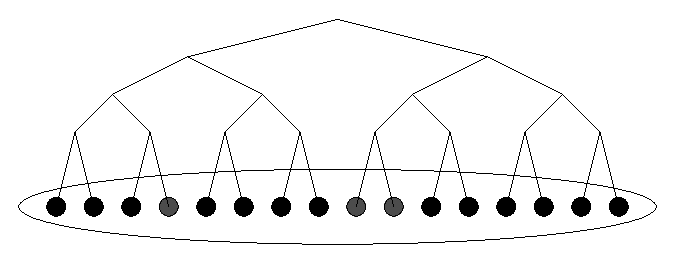
\includegraphics{search4.eps}
\end{center}
\caption{Search space structured using a search tree}
\label{figsearchtree}
\end{figure}
Figure \ref{figtreesearch} shows a sample tree search, namely a depth-first
incomplete traversal.
As opposed to that, figure \ref{figmovesearch} shows an example of an
incomplete move-based search which does not follow a fixed search space
structure. Of course, it will have to take other precautions to avoid
looping and ensure termination.
\begin{figure}
\begin{center}
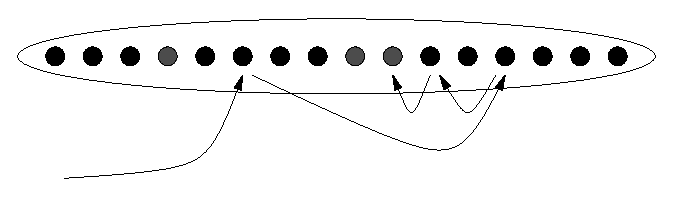
\includegraphics{search5.eps}
\end{center}
\caption{A move-based search}
\label{figmovesearch}
\end{figure}

\begin{figure}
\begin{center}
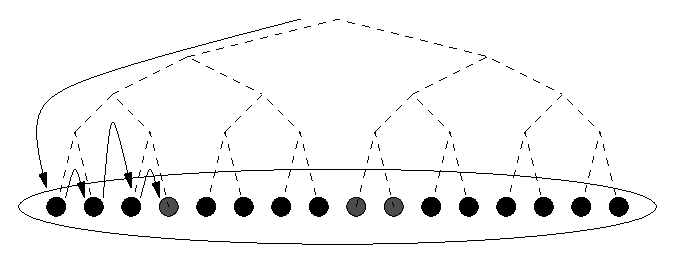
\includegraphics{search6.eps}
\end{center}
\caption{A tree search (depth-first)}
\label{figtreesearch}
\end{figure}

A few further observations:
Move-based methods are usually incomplete. This is not surprising given
typical sizes of search spaces.
A complete exploration of a huge search space
is only possible if large sub-spaces can be excluded a priory, and this
is only possible with constructive methods which allow to reason about
whole classes of similar assignments.
Moreover, a complete search method must remember which parts of the
search space have already been visited.
This can only be implemented with
acceptable memory requirements if there is a simple structuring of the
space that allows compact encoding of sub-spaces.


% - - - - - - - - - - - - - - - - - - - - - - - - - - - - - - - - - - -
\subsection{Optimisation and Search}
% - - - - - - - - - - - - - - - - - - - - - - - - - - - - - - - - - - -

Many practical problems are in fact optimisation problems, ie.\ we are
not just interested in some solution or all solutions, but in
the best solution.

Fortunately, there is a general method to find the optimal solution
based on the ability to find all solutions.
\index{branch-and-bound}
The {\em branch-and-bound} technique works are follows:
\begin{enumerate}
\item Find a first solution
\item Add a constraint requiring a better solution than the best
    one we have so far (e.g.\ require lower cost)
\item Find a solution which satisfies this new constraint.
    If one exists, we have a new best solution and we repeat step 2.
    If not, the last solution found is the proven optimum.
\end{enumerate}
The library {\bf branch\_and\_bound} provides the generic
branch-and-bound primitives bb\_min/3 and bb\_min/6.


% - - - - - - - - - - - - - - - - - - - - - - - - - - - - - - - - - - -
\subsection{Heuristics}
% - - - - - - - - - - - - - - - - - - - - - - - - - - - - - - - - - - -

Since search space sizes grow exponentially with problem size,
it is not possible to explore all assignments except for the
very smallest problems.
The only way out is {\em not} to look at the whole search space.
There are only two ways to do this:
\begin{itemize}
\item {\bf Prove} that certain areas of the space contain no solutions.
    This can be done with the help of constraints. This is often referred
    to as {\em pruning}\index{pruning}.
\item {\bf Ignore} parts of the search space that are unlikely to contain
    solutions (i.e.\ do incomplete search), or at least postpone their exploration.
    This is done by using {\em heuristics}\index{heuristics}.
    A heuristic is a particular traversal order of the search space
    which explores promising areas first.
\end{itemize}

In the following sections we will first investigate the considerable
degrees of freedom that are available for heuristics within the framework of
systematic tree search, which is the traditional search method
in the Constraint Logic Programming world.

Subsequently, we will turn our attention to move-based methods
which in {\eclipse} can be implemented using the facilities of the repair-library.


%----------------------------------------------------------------------
\section{Complete Tree Search with Heuristics}
%----------------------------------------------------------------------

There is one form of tree search which is especially economic: 
depth-first, left-to-right search by backtracking.  It allows to
traverse a search tree systematically while requiring only a stack
of maximum depth N for bookkeeping.  Most other strategies of tree
search (e.g.  breadth-first) have exponential memory requirements. 
This unique property is the reason why backtracking is a built feature
of {\eclipse}.  Note that the main disadvantage of the depth-first
strategy (the danger of going down an infinite branch) does not come
into play here because we deal with finite search trees.

Sometimes depth-first search and heuristic search are treated as antonyms.
This is only justified when the shape of the search tree is statically fixed.
Our case is different: we have the freedom of deciding on the shape of every
sub-tree before we start to traverse it depth-first. While this does not
allow to arrange for {\em any} order of visiting the leaves of the search tree,
it does provide considerable flexibility. This flexibility can be exploited
by variable and value selection strategies.

% - - - - - - - - - - - - - - - - - - - - - - - - - - - - - - - - - - -
\subsection{Search Trees}
% - - - - - - - - - - - - - - - - - - - - - - - - - - - - - - - - - - -

In general, the nodes of a search tree represent {\em choices}.
\index{choice}
These choices should be mutually exclusive and therefore partition the
\index{partition a search space}
search space into two or more disjoint sub-spaces.
In other words, the original problem is reduced to a disjunction
of simpler sub-problems.

In the case of finite-domain problems, the most common form of choice
is to choose a particular value for a problem variable
(this technique is often called
\index{labeling}
{\em labeling}).
For a boolean variable, this means setting the variable to 0 in one
branch of the search tree and to 1 in the other.
In {\eclipse}, this can be written as a disjunction
(which is implemented by backtracking):
\begin{quote}\begin{alltt}
( X1=0 ; X1=1 )
\end{alltt}\end{quote}
Other forms of choices are possible. If X2 is a variable that can take
integer values from 0 to 3 (assume it has been declared as \verb'X2::0..3'),
we can make a n-ary search tree node by writing
\begin{quote}\begin{alltt}
( X2=0 ; X2=1 ; X2=2 ; X2=3 )
\end{alltt}\end{quote}
or more compactly
\begin{quote}\begin{alltt}
indomain(X2)
\end{alltt}\end{quote}
However, choices do not necessarily involve choosing a concrete value
for a variable. It is also possible to make disjoint choices by
\index{domain splitting}
{\em domain splitting}, e.g.
\begin{quote}\begin{alltt}
( X2 #=< 1 ; X2 #>= 2 )
\end{alltt}\end{quote}
or by choosing a value in one branch and excluding it in the other:
\begin{quote}\begin{alltt}
( X2 = 0 ; X2 #>= 1 )
\end{alltt}\end{quote}
In the following examples, we will mainly use simple labeling,
which means that the search tree nodes correspond to a variable
and a node's branches correspond to the different values that the
variable can take.


% - - - - - - - - - - - - - - - - - - - - - - - - - - - - - - - - - - -
\subsection{Variable Selection}
% - - - - - - - - - - - - - - - - - - - - - - - - - - - - - - - - - - -

\begin{figure}
\begin{center}
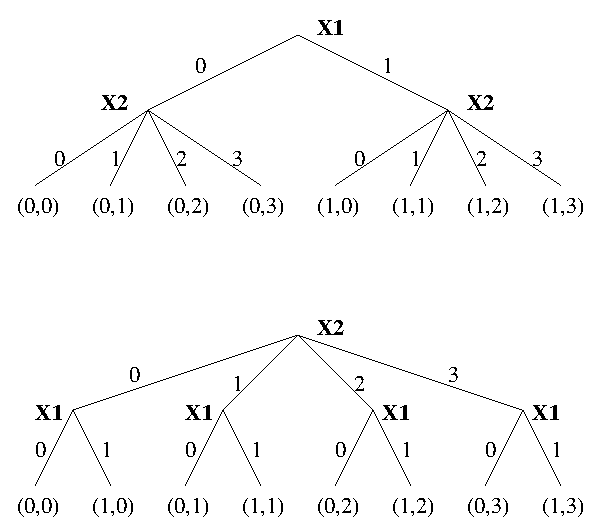
\includegraphics{search1.eps}
\end{center}
\caption{The effect of variable selection}
\label{figvarsel}
\end{figure}

Figure \ref{figvarsel} shows how variable selection reshapes a search tree.
If we decide to choose values for X1 first (at the root of the search tree)
and values for X2 second, then the search tree has one particular shape.
If we now assume a depth-first, left-to-right traversal by backtracking,
this corresponds to one particular order of visiting the leaves of the tree:
(0,0), (0,1), (0,2), (0,3), (1,0), (1,1), (1,2), (1,3).

If we decide to choose values for X2 first and X1 second, then the tree and
consequently the order of visiting the leaves is different:
(0,0), (1,0), (0,1), (1,1), (0,2), (1,2), (0,3), (1,3).

While with 2 variables there are only 2 variable selection strategies,
this number grows exponentially with the number of variables. For 5
variables there are already $2^{2^{5}-1} = 2147483648$ different variable selection
strategies to choose from.

Note that the example shows something else: If the domains of the variables
are different, then the variable selection can change the number of internal
nodes in the tree (but not the number of leaves). To keep the number of nodes
down, variables with small domains should be selected first.


% - - - - - - - - - - - - - - - - - - - - - - - - - - - - - - - - - - -
\subsection{Value Selection}
% - - - - - - - - - - - - - - - - - - - - - - - - - - - - - - - - - - -

The other way to change the search tree is value selection, i.e. reordering
the child nodes of a node by choosing the 
values from the domain of a variable in a particular order.
Figure \ref{figvalsel} shows how this can change the order of visiting the
leaves:
(1,2), (1,1), (1,0), (1,3), (0,1), (0,3), (0,0), (0,2).

\begin{figure}
\begin{center}
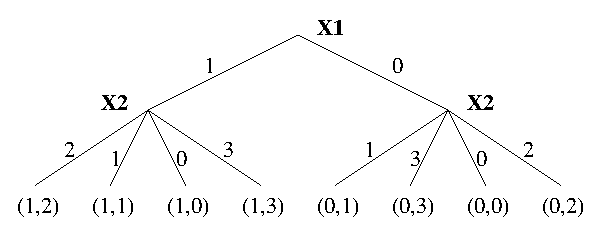
\includegraphics{search2.eps}
\end{center}
\caption{The effect of value selection}
\label{figvalsel}
\end{figure}

By combining variable and value selection, a large number of different
heuristics can be implemented.
To give an idea of the numbers involved, the following table shows the search
space sizes, the number of possible search space traversal orderings,
and the number of orderings
that can be obtained by variable and value selection (assuming domain size 2).

\enableunderscores
\begin{center}
\begin{tabular}{|l|l|l|l|}
\hline
Variables&      Search space&   Visiting orders&        Selection Strategies\\
\hline
1&              2&                      2&              2\\
2&              4&                      24&             16\\
3&              8&                      40320&          336\\
4&              16&                     $2.1*10^{13}$&  $1.8*10^7$\\
5&              32&                     $2.6*10^{35}$&  $3.5*10^{15}$\\
n&              $2^n$&          $2^n!$& 
                                $2^{{2^n}-1} \prod_{i=0}^{n-1} (n-1)^{2^i}$\\
\hline
\end{tabular}
\end{center}
\disableunderscores

% - - - - - - - - - - - - - - - - - - - - - - - - - - - - - - - - - - -
\subsection{Example}
% - - - - - - - - - - - - - - - - - - - - - - - - - - - - - - - - - - -

We use the famous N-Queens problem to illustrate how heuristics can be applied
to backtrack search through variable and value selection.
We model the problem with one variable per queen, assuming that each queen
occupies one colunm. The variables range from 1 to N and indicate the row
in which the queen is being placed. The constraints ensure that no two
queens occupy the same row or diagonal:
%!!!!!!!!!!!!!!!!!!!!!!!!!!!!!!!!!!!!!!!!!!!!!!!!!!
% CAUTION: I use the old ## syntax here because
% #\= is not treated correctly by latex2html
%!!!!!!!!!!!!!!!!!!!!!!!!!!!!!!!!!!!!!!!!!!!!!!!!!!
\begin{quote}\begin{alltt}
:- lib(fd).

queens(N, Board) :-
        length(Board, N),
        Board :: 1..N,
        ( fromto(Board, [Q1|Cols], Cols, []) do
            ( foreach(Q2, Cols), count(Dist,1,_), param(Q1) do
                noattack(Q1, Q2, Dist)
            )
        ).

    noattack(Q1,Q2,Dist) :-
        Q2 ## Q1,
        Q2 - Q1 ## Dist,
        Q1 - Q2 ## Dist.
\end{alltt}\end{quote}
We are looking for a first solution to the 16-queens problem by calling
\begin{quote}\begin{alltt}
?- queens(16, Vars),   % model
   labeling(Vars).     % search
\end{alltt}\end{quote}
We start naively, using the pre-defined labeling-predicate that comes with the
finite-domain library. It is defined as follows:
\begin{quote}\begin{alltt}
labeling(AllVars) :-
        ( foreach(Var, AllVars) do
            indomain(Var)                       % select value
        ).
\end{alltt}\end{quote}
The strategy here is simply to select the variables
from left to right as they occur in the list, and they are
assigned values starting from the lowest to the numerically highest they can
take (this is the definition of indomain/1).
A solution is found after 542 backtracks
(see section \ref{countbt} below for how to count backtracks).

A first improvement is to employ a
{\bf general-purpose variable-selection heuristic},
\index{first-fail principle}
the so called first-fail principle. It requires to label the
variables with the smallest domain first. This reduces the branching
factor at the root of the search tree and the total number of internal nodes.
The deleteff/3 predicate implements this strategy for finite domains.
Using deleteff/3, we can redefine our labeling-routine as follows:
\begin{quote}\begin{alltt}
labeling(AllVars) :-
        ( fromto(AllVars, Vars, VarsRem, []) do
            deleteff(Var, Vars, VarsRem),       % dynamic var-select
            indomain(Var)                       % select value
        ).
\end{alltt}\end{quote}
Indeed, for the 16-queens example, this leads to a dramatic improvement,
the first solution is found with only 3 backtracks now.
But caution is necessary: The 256-queens instance for example solves
nicely with the naive strategy, but our improvement leads to a
disappointment: the time increases dramatically!
This is not uncommmon with heuristics: one has to keep in mind that the
search space is not reduced, just re-shaped. Heuristics that yield good
results with some problems can be useless or counter-productive with others.
Even different instances of the same problem can exhibit widely different
characteristics.
 
Let us try to employ a {\bf problem-specific heuristic}:
Chess players know that pieces in the middle of the board are more
useful because they can attack more fields. We could therefore start
placing queens in the middle of the board to reduce the number of
unattacked fields earlier. We can achieve that simply by pre-ordering the
variables such that the middle ones are first in the list:
\begin{quote}\begin{alltt}
labeling(AllVars) :-
        middle_first(AllVars, AllVarsPreOrdered), % static var-select
        ( foreach(Var, AllVarsPreOrdered) do
            indomain(Var)                       % select value
        ).
\end{alltt}\end{quote}
The implementation of middle\_first/2 requries a bit of list manipulation
and uses primitives from the lists-library:
\begin{quote}\begin{alltt}
:- lib(lists).

middle_first(List, Ordered) :-
        halve(List, Front, Back),
        reverse(Front, RevFront),
        splice(Back, RevFront, Ordered).
\end{alltt}\end{quote}
This strategy also improves things for the 16-queens instance, the
first solution requires 17 backtracks.

We can now improve things further by {\bf combining} the two
variable-selection strategies:
When we pre-order the variables such that the middle ones are first,
the deleteff/3 predicate will prefer middle variables when several
have the same domain size:
\begin{quote}\begin{alltt}
labeling(AllVars) :-
        middle_first(AllVars, AllVarsPreOrdered), % static var-select
        ( fromto(AllVarsPreOrdered, Vars, VarsRem, []) do
            deleteff(Var, Vars, VarsRem),       % dynamic var-select
            indomain(Var)                       % select value
        ).
\end{alltt}\end{quote}
The result is positive: for the 16-queens instance,
the number of backtracks goes down to zero,
and more difficult instances become solvable!

Actually, we have not yet implemented our intuitive heuristics properly.
We start placing queens in the middle columns, but not on the middle rows.
With our model, that can only be achieved by {\bf changing the value selection},
ie.\ setting the variables to values in the middle of their domain.
We therefore invent a variant of indomain/1 called middle\_first\_indomain/1
and the resulting labeling routine then looks as follows:
\begin{quote}\begin{alltt}
labeling(AllVars) :-
        middle_first(AllVars, AllVarsPreOrdered), % static var-select
        ( fromto(AllVarsPreOrdered, Vars, VarsRem, []) do
            deleteff(Var, Vars, VarsRem),       % dynamic var-select
            middle_first_indomain(Var)          % select value
        ).
\end{alltt}\end{quote}
The implementation of middle\_first\_indomain/2
simply relies on middle\_first/2:
\begin{quote}\begin{alltt}
middle_first_indomain(X) :-
        nonvar(X).
middle_first_indomain(X) :-
        var(X),
        dom(X, List),    % the list of values in X's domain
        middle_first(List, Ordered),
        member(X, Ordered).
\end{alltt}\end{quote}
Surprisingly, this improvement again increases the backtrack count for
16-queens again to 3.
However, when looking at a number of different instances of the problem,
we can observe that the overall behaviour has improved and the
performance has become more predictable than with the
initial more naive strategies.


% - - - - - - - - - - - - - - - - - - - - - - - - - - - - - - - - - - -
\subsection{Counting Backtracks}
% - - - - - - - - - - - - - - - - - - - - - - - - - - - - - - - - - - -

%The size of the (remaining) search space can be computed easily
%in finite-domain problems. All we have to do is to multiply the
%sizes of all the (remaining) variable's domains:
%\begin{quote}\begin{alltt}
%search_space(Vars, Size) :-
%        ( foreach(V,Vars), fromto(1,S0,S1,Size) do
%            dvar_domain(V,D), S1 is S0*dom_size(D)
%        ).
%\end{alltt}\end{quote}

\label{countbt}
An interesting piece of information during program development is the
number of backtracks. It is a good measure for the quality of
both constraint propagation and search heuristics.
We can instrument our labeling routine as follows:
\begin{quote}\begin{alltt}
labeling(AllVars) :-
        init_backtracks,
        ( foreach(Var, AllVars) do
            count_backtracks,       % insert this before choice!
            indomain(Var)
        ),
        get_backtracks(B),
        printf("Solution found after %d backtracks%n", [B]).
\end{alltt}\end{quote}
The backtrack counter itself can be implemented by the code below.
It uses a non-logical counter variable (backtracks) and an additional
flag (deep\_fail) which ensures that backtracking to exhausted choices
does not increment the count.
\begin{quote}\begin{alltt}
:- local variable(backtracks), variable(deep_fail).

init_backtracks :-
        setval(backtracks,0).

get_backtracks(B) :-
        getval(backtracks,B).

count_backtracks :-
        setval(deep_fail,false).
count_backtracks :-
        getval(deep_fail,false),        % may fail
        setval(deep_fail,true),
        incval(backtracks),
        fail.
\end{alltt}\end{quote}
Note that there are other possible ways of defining the number of backtracks.
However, the one suggested here has the following useful properties:
\begin{itemize}
\item Shallow backtracking (an attempt to instantiate a variable which
    causes immediate failure due to constraint propagation) is not counted.
    If constraint propagation works well, the count is therefore zero.
\item With a perfect heuristic, the first solution is found with zero
    backtracks.
\item If there are N solutions, the best achievable value is N (one backtrack
    per solution). Higher values indicate an opportunity to improve pruning
    by constraints.
\end{itemize}


%----------------------------------------------------------------------
\section{Incomplete Tree Search}
%----------------------------------------------------------------------
%\subsection{Pruning with Extra Constraints}
%\subsection{First Solution}

% - - - - - - - - - - - - - - - - - - - - - - - - - - - - - - - - - - -
\subsection{Bounded Backtrack Search} 
% - - - - - - - - - - - - - - - - - - - - - - - - - - - - - - - - - - -

One way to limit the scope of backtrack search is to keep a
record of the number of backtracks, and curtail the search when this
limit is exceeded.

You can find an implementation of Bounded Backtrack Search ({\em BBS})
in the file {\tt lds.ecl} in the {\tt doc/examples} directory of your
{\eclipse} installation.
The predicate defining bounded backtrack search is
\verb0bounded_backtrack_search0, and it takes two arguments, a list of
variables and an integer (the limit on the number of backtracks).
An example invocation is:
\begin{quote}\begin{alltt}
?- [X,Y,Z]::1..3, X+Y+Z#=6, bounded_backtrack_search([X,Y,Z],4).
\end{alltt}\end{quote}
The answers are returned on backtracking in the following order:
\begin{itemize}
\item
X = 1
Y = 2
Z = 3
\item
X = 1
Y = 3
Z = 2  
\item
X = 2
Y = 1
Z = 3
\item
X = 2
Y = 2
Z = 2    
\end{itemize}
After which the procedure fails outputting
\verb0Backtrack limit exceeded0.

The implementation uses several
facilities of {\eclipse}, including {\em non-logical variables} and
{\em catch and throw}:
\begin{quote}\begin{alltt}
:- local variable(backtracks), variable(deep_fail).

bounded_backtrack_search(List,Limit) :-
        setval(backtracks,Limit),
        block(bbs_label(List),
              exceed_limit,
              (writeln('Backtrack limit exceeded'), fail)
             ).

bbs_label([]).
bbs_label([Var|Vars]) :-
        limit_backtracks,
        indomain(Var),
        bbs_label(Vars).
    
limit_backtracks :-
        setval(deep_fail,false).
limit_backtracks :-
        getval(deep_fail,false),        % may fail
        setval(deep_fail,true),
        decval(backtracks),
        (getval(backtracks,0) -> exit_block(exceed_limit) ; fail).
\end{alltt}\end{quote}


% - - - - - - - - - - - - - - - - - - - - - - - - - - - - - - - - - - -
\subsection{Credit Search}
% - - - - - - - - - - - - - - - - - - - - - - - - - - - - - - - - - - -

Credit search is a tree search method where the number of
nondeterministic choices is limited a priori.  This is achieved by
starting the search at the tree root with a certain integral amount of
credit.  This credit is split between the child nodes, their credit
between their child nodes, and so on.  A single unit of credit cannot
be split any further: subtrees provided with only a single credit unit
are not allowed any nondeterministics choices, only one path though these
subtrees can be explored, i.e. only one leaf in the subtree can be visited.
Subtrees for which no credit is left are pruned,
i.e.\ not visited.

The following code (a replacement for labeling/1)
implements credit search. For ease of understanding, it is
limited to boolean variables:
\begin{quote}\begin{alltt}
% Credit search (for boolean variables only)
credit_search(Credit, Xs) :-
        (
            foreach(X, Xs),
            fromto(Credit, ParentCredit, ChildCredit, _)
        do
            ( var(X) ->
                ParentCredit > 0,  % possibly cut-off search here
                ( % Choice
                    X = 0, ChildCredit is (ParentCredit+1)//2
                ;
                    X = 1, ChildCredit is ParentCredit//2
                )
            ;
                ChildCredit = ParentCredit
            )
        ).
\end{alltt}\end{quote}
Note that the leftmost alternative (here X=0)
gets slightly more credit than the rightmost one (here X=1)
by rounding the child node's credit up rather than down. 
This is especially relevant when the leftover credit is down to 1:
from then on, only the leftmost alternatives will be taken until a
leaf of the search tree is reached. The leftmost alternative should
therefore be the one favoured by the search heuristics.

What is a reasonable amount of credit to give to a search?
In an unconstrained search tree, the credit is equivalent to the
number of leaf nodes that will be reached.
The number of leaf nodes grows exponentially with the number of
labelled variables, while tractable computations should have
polynomial runtimes. A good rule of thumb could therefore be to
use as credit the number of variables squared or cubed, thus enforcing
polynomial runtime.

Note that this method in its pure form allow choices only close to the
root of the search tree and disallows choices completely below a certain
tree depth. This is too restrictive when the value selection strategy
is not good enough. A possible remedy is to combine credit search with
bounded backtrack search.


% - - - - - - - - - - - - - - - - - - - - - - - - - - - - - - - - - - -
\subsection{Timeout}
% - - - - - - - - - - - - - - - - - - - - - - - - - - - - - - - - - - -

Another form of incomplete tree search is simply to use time-outs.
The branch-and-bound primitives min\_max/6,8 and minimize/6,8 allow
to specify a maximal runtime. If a timeout occurs, the best solution
found so far is returned instead of the proven optimum.

A general timeout can be implemented as follows. When Goal has run for
more than Seconds seconds, it is aborted and TimeOutGoal is called instead.
\begin{quote}\begin{alltt}
:- set_event_handler(timeout, exit_block/1).

timeout(Goal, Seconds, TimeOutGoal) :-
        block(
            timeout_once(Goal, Seconds),
            timeout,
            call(TimeOutGoal)
        ).

    timeout_once(Goal, Seconds) :-
        event_after(timeout, Seconds),
        ( call(Goal) ->
            cancel_after_event(timeout)
        ;
            cancel_after_event(timeout),
            fail
        ).
\end{alltt}\end{quote}


%----------------------------------------------------------------------
\subsection{Limited Discrepancy Search}
%----------------------------------------------------------------------

% - - - - - - - - - - - - - - - - - - - - - - - - - - - - - - - - - - -
\subsubsection{Introduction}
% - - - - - - - - - - - - - - - - - - - - - - - - - - - - - - - - - - -

Limited discrepancy search ({\em LDS}) is a search method that assumes
the user has a good heuristic for directing the search.  A perfect
heuristic would, of course, not require any search.  However most
heuristics are occasionally misleading.  Limited Discrepancy Search
follows the heuristic on almost every decision.  The
``discrepancy'' is a measure of the degree to which it fails to follow
the heuristic.  LDS starts searching with a discrepancy of $0$ (which
means it follows the heuristic exactly).  Each time LDS fails to find
a solution with a given discrepancy, the discrepancy is increased and
search restarts.  In theory the search is complete, as eventually the
discrepancy will become large enough to admit a solution, or cover
the whole search space.  In practice, however, it is only beneficial
to apply LDS with small discrepancies.  Subsequently, if no solution
is found, other search methods should be tried.

The definitive reference to LDS is:
\begin{quote}
Limited Discrepancy Search, Harvey and Ginsberg,
pp.607-613, Proc. IJCAI'95
\end{quote}

This reference also suggests that combining LDS with Bounded Backtrack
Search ({\em BBS}) yields good behaviour.  Accordingly the {\eclipse} LDS
module also supports BBS and its combination with LDS.

% - - - - - - - - - - - - - - - - - - - - - - - - - - - - - - - - - - -
\subsubsection{Limited Discrepancy Search using a Static Heuristic}
% - - - - - - - - - - - - - - - - - - - - - - - - - - - - - - - - - - -

We start by assuming a static heuristic, which is a complete
assignment to the problem variables specified in advance of the
search.  The predicate supporting static LDS takes a list of variables
(those which are to be labelled) and a list of values (one heuristic
value for each variable, respectively).  Each variable has a finite
domain, and its heuristic value should belong to its domain (though
the LDS search can still succeed even if this is not the case).

The measure of discrepancy, in this case, is simply the number of
variables labelled differently to the heuristic.  Thus the maximum
discrepancy is just the number of variables to be
labelled.

LDS search is implemented in the file
{\tt lds.ecl} in the {\tt doc/examples} directory of your
{\eclipse} installation. You can copy this file and load it with
\begin{quote}\begin{alltt}
:- use_module(lds).
\end{alltt}\end{quote}
Static LDS search is then available via the predicate
{\bf static_lds(Var, Vals, Discrepancy)} whose arguments are
\begin{description}
\item[Vars] the list of problem variables.  Some of the
variables may already be instantiated.  The others
must have associated finite domains.
\item[Vals] the list of values according to the heuristic.  It
must be the same length as Vars, and the heuristic
must match the value, in case the variable is
already instantiated.
\item[Discrepancy] the discrepancy of the solution returned.  Typically this
is an output of the search (an integer between $0$ and the number of
variables), but it can also be used as an input.
\end{description}
The finite domain library must be loaded, and the variables must have
finite domains.  An example invocation is:
\begin{quote}\begin{alltt}
?- [X,Y,Z]::1..3, X+Y+Z#=5, static_lds([X,Y,Z],[1,2,3],D).
\end{alltt}\end{quote}
The answers are returned on backtracking in the following order:
\begin{itemize}
\item
X = 1
Y = 2
Z = 2
D = 1     
\item
X = 1
Y = 1
Z = 3
D = 1     
\item
X = 1
Y = 3
Z = 1
D = 2     
\item
X = 2
Y = 2
Z = 1
D = 2     
\item
X = 2
Y = 1
Z = 2
D = 3     
\item
X = 3
Y = 1
Z = 1
D = 3
\end{itemize}


% - - - - - - - - - - - - - - - - - - - - - - - - - - - - - - - - - - -
\subsubsection{Limited Discrepancy Search using a Dynamic Heuristic}
% - - - - - - - - - - - - - - - - - - - - - - - - - - - - - - - - - - -

Often the heuristic value is calculated on the fly, during search.  To
cope with this we use the {\eclipse} ``tentative value'' facility in
{\eclipse}'s {\em repair} library. 
The heuristic is stored with the variable as its tentative value. 

The tentative value may be changed during search.  For example if a
variable is instantiated as a consequence of constraint propagation
during search, its tentative value is automatically changed to its
actual value. 

Dynamic LDS search is available in {\eclipse} via the predicate
{\bf dynamic_lds(Vars, Discrepancy)}.
Each variable in the list of variables {\em Vars} 
must have a tentative value.

An example invocation is:
\begin{quote}\begin{alltt}
?- [X,Y,Z]::1..3, [X,Y,Z] tent_set [1,2,3], X+Y+Z#=5,
   dynamic_lds([X,Y,Z],D).
\end{alltt}\end{quote}
The answers are returned on backtracking in the following order.
Notice that the first solution has a discrepancy of $0$, because
constraint propagation instantiates the third variable to $2$,
thus changing its tentative value from $3$ to $2$.
\begin{itemize}
\item
X = 1
Y = 2
Z = 2
D = 0    
\item
X = 1
Y = 1
Z = 3
D = 1    
\item
X = 1
Y = 3
Z = 1
D = 1    
\item
X = 2
Y = 2
Z = 1
D = 1    
\item
X = 3
Y = 1
Z = 1
D = 1    
\item
X = 2
Y = 1
Z = 2
D = 2 
\end{itemize}

% - - - - - - - - - - - - - - - - - - - - - - - - - - - - - - - - - - -
\subsubsection{LDS and BBS Combined}
% - - - - - - - - - - - - - - - - - - - - - - - - - - - - - - - - - - -

The two search techniques, BBS and LDS, can be merged quite simply in
{\eclipse}, so that for each discrepancy level only a limited number of
backtracks are allowed.  

An example invocation is:
\begin{quote}\begin{alltt}
?- Vars=[X,Y,Z], Vars::1..3, Vars tent_set [1,2,3], X+Y+Z#=6,
   bbs_dynamic_lds(Vars,4,D).
\end{alltt}\end{quote}
The answers are returned on backtracking in the following order:
\begin{itemize}
\item
X = 1
Y = 2
Z = 3
D = 0   
\item
X = 1
Y = 3
Z = 2
D = 1   
\item
X = 2
Y = 2
Z = 2
D = 1   
\item
X = 3
Y = 2
Z = 1
D = 1   \\
Backtrack limit exceeded
\item
X = 2
Y = 1
Z = 3
D = 2 \\
Backtrack limit exceeded
\end{itemize}

%----------------------------------------------------------------------
\section{Local Search Methods}
%----------------------------------------------------------------------

In the following we discuss several examples of move-based (as opposed
to constructive search) methods. These methods have originally been developed
for unconstrained problems, but they work for certain classes of
constrained problems as well.

From a technical point of view, the main difference between tree search
and move-based search is that tree search is monotonic in the sense that
constraints get tightened when going down the tree, and this is undone
in reverse order when backing up the tree to a parent node. This fits
well with the idea of constraint propagation.
In a move-based search, the main characteristics is that a move produces
a small change, but it is not clear what effect this will have on the
constraints. They may become more or less satisfied.
We therefore need implementations of the constraints that monitor changes
rather than propagate instantiations. This functionality is provided by
the {\eclipse} repair library which is used in the following examples.
The repair library is decribed in more detail in the
{\eclipse} Constraint Library Manual.
 
The {\eclipse} code for all the examples in this section is available
in the file {\tt knapsack_ls.ecl} in the {\tt doc/examples} directory of your
{\eclipse} installation.

% - - - - - - - - - - - - - - - - - - - - - - - - - - - - - - - - - - -
\subsection{The Knapsack Example}
% - - - - - - - - - - - - - - - - - - - - - - - - - - - - - - - - - - -

We will demonstrate the local search methods using the well-known
knapsack problem. The problem is the following: given a container of
a given capacity and a set of items with given weights and profit
values, find out which items have to be packed into the container
such that their weights do not exceed the container's capacity and
the sum of their profits is maximal.

The model for this problem involves N boolean variables, a single
inequality constraint to ensure the capacity restriction, and an
equality to define the objective function.

The tree search program for this problem looks as follows:
\begin{quote}\begin{alltt}
:- lib(fd).
knapsack(N, Profits, Weights, Capacity, Profit) :-
        length(Vars, N),                    % N boolean variables
        Vars :: 0..1,
        Capacity #>= Weights*Vars,          % the single constraint
        Profit #= Profits*Vars,             % the objective
        min_max(labeling(Vars), -Profit).   % branch-and-bound search
\end{alltt}\end{quote}
At the end of the problem modelling code, a standard branch-and-bound tree search
(min_max) is invoked in the last line of the code.
The parameters mean
\begin{itemize}
\item {\tt N} - the number of items (integer)
\item {\tt Profits} - a list of N integers (profit per item)
\item {\tt Weights} - a list of N integers (weight per item)
\item {\tt Capacity} - the capacity of the knapsack (integer)
\item {\tt Opt} - the optimal result (output)
\end{itemize}
To be able to use local search, we load the {\bf repair} library and
change the problem setup slightly.
At the end, we invoke a local search routine instead of tree search:
\begin{quote}\begin{alltt}
:- lib(fd).
:- lib(repair).
knapsack(N, Profits, Weights, Capacity, Opt) :-
        length(Vars, N),
        Vars :: 0..1,
        Capacity #>= Weights*Vars  r_conflict cap,
        Profit tent_is Profits*Vars,
        local_search(<extra parameters>, Vars, Profit, Opt).
\end{alltt}\end{quote}
We are now using 3 features from the repair-library:
\begin{description}
\item[Constraint annotation r\_conflict:] Constraints annotated in this
        way are constantly being monitored for satifying the global
        assignment, i.e. it is checked whether they would be satisfied
        if all variables were instantiated to their tentative values.
        Constraints that are not satisfied in this way appear in the
        specified {\em conflict set}.
        In the example, the single capacity constraint has been annotated with
        {\bf r\_conflict} and it will appear in the conflict set called
        {\tt cap} when violated.
\item[Result tent\_is ArithExpression:] This is similar to the is/2 built-in
        predicate, but it works on the variable's tentative values rather
        than requiring the variables to be instantiated. The result is
        delivered as the tentative value of Result. Any change of tentative
        value inside the ArithExpression leads to an update of the Result.
        In the example, the computation of the objective function has
        been changed to use {\bf tent\_is} because we want to have the
        objective value recomputed efficiently after every move.
\item[Tentative values:] Every variable has, apart from its domain,
        a tentative value which can be changed using tent\_set/2 and
        queried using tent\_get/2. We will use these inside the local search
        routine to implement the moves.
\end{description}


% - - - - - - - - - - - - - - - - - - - - - - - - - - - - - - - - - - -
\newpage
\subsection{Search Code Schema}
% - - - - - - - - - - - - - - - - - - - - - - - - - - - - - - - - - - -

In the literature, e.g.\ in
\begin{quote}
Localizer: A Modeling Language for Local Search,
L. Michel and P. Van Hentenryck, Proceeding CP97, LNCS 1330, Springer 1997.
\end{quote}
local search methods are often characterised by
the the following nested-loop program schema:
\begin{quote}\begin{alltt}
local_search:
     set starting state
     while global_condition
         while local_condition
             select a move
             if acceptable
                 do the move
                 if new optimum
                     remember it
         endwhile
         set restart state
     endwhile
\end{alltt}\end{quote}
The actual program codes in the following sections all follow this schema,
except that some methods (random walk and the tabu search)
are even simpler and use only a single loop with a single termination
condition.


%----------------------------------------------------------------------
\newpage
\subsection{Random walk}
%----------------------------------------------------------------------

As a simple example of local search, let us look at a random walk
strategy.  The idea is to start from a random tentative assignment of
variables to 0 (item not in knapsack) or 1 (item in knapsack), then to
remove random items (changing 1 to 0) if the knapsack's capacity is
exceeded and to add random items (changing 0 to 1) if there is
capacity left.  We do a fixed number (MaxIter) of such steps and keep
track of the best solution encountered.

Each step consists of
\begin{itemize}
\item Changing the tentative value of some variable, which in turn causes
        the automatic recomputation of the conflict constraint set
        and the tentative objective value.
\item Checking whether the move lead to a solution and whether this
        solution is better than the best one so far.
\end{itemize}

Here is the {\eclipse} program. We assume that the problem has been set
up as explained above. The violation of the capacity constraint
is checked by looking at the conflict constraints. If there are no
conflict constraints, the constraints are all tentatively satisfied
and the current tentative values form a solution to the problem.
The associated profit is obtained by looking at the tentative value
of the Profit variable (which is being constantly updated by tent\_is).
\begin{quote}\begin{alltt}
random_walk(MaxIter, VarArr, Profit, Opt) :-
        init_tent_values(VarArr, random),       % starting point
        (   for(_,1,MaxIter),                   % do MaxIter steps
            fromto(0, Best, NewBest, Opt),      % track the optimum
            param(Profit,VarArr)
        do
            ( conflict_constraints(cap,[]) ->   % it's a solution!
                Profit tent_get CurrentProfit,  % what is its profit?
                (
                    CurrentProfit > Best        % new optimum?
                ->
                    printf("Found solution with profit %w%n", [CurrentProfit]),
                    NewBest=CurrentProfit       % yes, remember it
                ;
                    NewBest=Best                % no, ignore
                ),
                change_random(VarArr, 0, 1)     % add another item
            ;
                NewBest=Best,
                change_random(VarArr, 1, 0)     % remove an item
            )
        ).
\end{alltt}\end{quote}
The auxiliary predicate {\tt init_tent_values} sets the tentative values
of all variables in the array randomly to 0 or 1:
The {\tt change_random} predicate changes a randomly selected variable with
a tentative value of 0 to 1, or vice versa.
Note that we are using an array, rather than a list of variables, to
provide more convenient random access.
The complete code and the auxiliary predicate definitions can be found
in the file {\tt knapsack_ls.ecl} in the {\tt doc/examples} directory of your
{\eclipse} installation.


%----------------------------------------------------------------------
\subsection{Hill Climbing}
%----------------------------------------------------------------------

The following hill-climbing implementation is an instance of the nested
loop program schema introduced above.  The idea is to start from
a configuration which is certainly a solution (the empty knapsack)
and do random uphill moves for at most MaxIter times. Then we restart
and try again:
\begin{quote}\begin{alltt}
hill_climb(MaxTries, MaxIter, VarArr, Profit, Opt) :-
        init_tent_values(VarArr, 0),            % starting solution
        (
            for(I,1,MaxTries),
            fromto(0, Opt1, Opt4, Opt),
            param(MaxIter,Profit,VarArr)
        do
            (
                for(J,1,MaxIter),
                fromto(Opt1, Opt2, Opt3, Opt4),
                param(I,VarArr,Profit)
            do
                Profit tent_get PrevProfit,
                (
                    flip_random(VarArr),        % try a move
                    Profit tent_get CurrentProfit,
                    CurrentProfit > PrevProfit, % is it uphill?
                    conflict_constraints(cap,[])  % is it a solution?
                ->
                    ( CurrentProfit > Opt2 ->   % is it new optimum?
                        printf("Found solution with profit %w%n",
                                    [CurrentProfit]),
                        Opt3=CurrentProfit      % accept and remember
                    ;
                        Opt3=Opt2               % accept
                    )
                ;
                    Opt3=Opt2                   % reject (move undone)
                )
            ),
            init_tent_values(VarArr, 0)         % restart
        ).
\end{alltt}\end{quote}
The move operator is implemented as follows. It chooses a random variable X
from the array of variables and changes its tentative value from 0 to 1
or from 1 to 0 respectively:
\begin{quote}\begin{alltt}
flip_random(VarArr) :-
        functor(VarArr, _, N),
        X is VarArr[random mod N + 1],
        X tent_get Old,
        New is 1-Old,
        X tent_set New.
\end{alltt}\end{quote}
Some further points are worth noticing:
\begin{itemize}
\item The move operation and the acceptance test
are within the condition part of the if-then-else construct.
As a consequence, if the acceptance test fails (the move either yields
no solution or does not improve the objective) the move is automatically
undone by backtracking.
\item To check whether the move is uphill, we retrieve the tentative
value of the Profit-variable before and after the move is done. 
Remember that, since the move operator changes the tentative values of
some variable, the tent\_is/2 primitive will automatically
update the Profit variable.
\item As in the random walk example, constraint satisfaction is checked
by checking whether the conflict constraint set is empty.
\end{itemize}

%----------------------------------------------------------------------
\newpage
\subsection{Simulated Annealing}
%----------------------------------------------------------------------

Simulated Annealing is a slightly more complex variant of local search.
It follows the schema in figure \ref{figmovesearch} and uses the same
move operator as the hill-climbing example.
The differences are in the termination conditions and in the
acceptance criterion for a move.
The outer loop simulates the cooling process by reducing the temperature
variable T, the inner loop does random moves until MaxIter steps have been
done without improvement of the objective.
The acceptance criterion is the classical one for simulated annealing:
Uphill moves are always accepted, downhill moves with a probability
that decreases with the temperature. The search routine must be invoked
with appropriate start and end temperatures, they should roughly correspond
to the maximum and minimum profit changes that a move can incur.
\begin{quote}\begin{alltt}
sim_anneal(Tinit, Tend, MaxIter, VarArr, Profit, Opt) :-
        starting_solution(VarArr),              % starting solution
        (   fromto(Tinit, T, Tnext, Tend),
            fromto(0, Opt1, Opt4, Opt),
            param(MaxIter,Profit,VarArr,Tend)
        do
            printf("Temperature is %d%n", [T]),
            (    fromto(MaxIter, J0, J1, 0),
                fromto(Opt1, Opt2, Opt3, Opt4),
                param(VarArr,Profit,T)
            do
                Profit tent_get PrevProfit,
                (   flip_random(VarArr),        % try a move
                    Profit tent_get CurrentProfit,
                    exp((CurrentProfit-PrevProfit)/T) > frandom,
                    conflict_constraints(cap,[])   % is it a solution?
                ->
                    ( CurrentProfit > Opt2 ->   % is it new optimum?
                        printf("Found solution with profit %w%n",
                                    [CurrentProfit]),
                        Opt3=CurrentProfit,     % accept and remember
                        J1=J0
                    ; CurrentProfit > PrevProfit ->
                        Opt3=Opt2, J1=J0        % accept
                    ;
                        Opt3=Opt2, J1 is J0-1   % accept
                    )
                ;
                    Opt3=Opt2, J1 is J0-1       % reject
                )
            ),
            Tnext is max(fix(0.8*T),Tend)
        ).
\end{alltt}\end{quote}

%----------------------------------------------------------------------
\newpage
\subsection{Tabu Search}
%----------------------------------------------------------------------
Another variant of local search is tabu search.  Here, a number of moves
(usually the recent moves) are remembered (the tabu list) to direct the
search. Moves are selected by an acceptance criterion, with a 
different (generally stronger) acceptance crtierion for moves in the tabu
list.  As in most local search methods there are many possible variants and
concrete instances of this basic idea. For example, how a move would be
added to or removed from the tabu list has to be specified, along with the
different acceptance criteria.

In the following simple example, the tabu list has a length determined by
the parameter TabuSize. The local moves consist of either adding
the item with the best relative profit into the knapsack, or removing
the worst one from the knapsack. In both cases, the move gets rememebered
in the fixed-size tabu list, and the complementary move is forbidden
for the next TabuSize moves.
\begin{quote}\begin{alltt}
tabu_search(TabuSize, MaxIter, VarArr, Profit, Opt) :-
        starting_solution(VarArr),              % starting solution
        tabu_init(TabuSize, none, Tabu0),
        (   fromto(MaxIter, I0, I1, 0),
            fromto(Tabu0, Tabu1, Tabu2, _),
            fromto(0, Opt1, Opt2, Opt),
            param(VarArr,Profit)
        do
            (   try_set_best(VarArr, MoveId),   % try uphill move
                conflict_constraints(cap,[]),   % is it a solution?
                tabu_add(MoveId, Tabu1, Tabu2)  % is it allowed?
            ->
                Profit tent_get CurrentProfit,
                ( CurrentProfit > Opt1 ->       % is it new optimum?
                    printf("Found solution with profit %w%n", [CurrentProfit]),
                    Opt2=CurrentProfit          % accept and remember
                ;
                    Opt2=Opt1                   % accept
                ),
                I1 is I0-1
            ;
                (   try_clear_worst(VarArr, MoveId),    % try downhill move
                    tabu_add(MoveId, Tabu1, Tabu2)      % is it allowed?
                ->
                    I1 is I0-1,
                    Opt2=Opt1                   % reject
                ;
                    I1=0,                       % no moves possible, stop
                    Opt2=Opt1                   % reject
                )
            )
        ).
\end{alltt}\end{quote}

In practice, the tabu search forms only a skeleton around which a complex
search algorithm is built. An example of this is applying tabu search to
the job-shop problem, as described by Nowicki and Smutnicki ({\it A Fast
Taboo Search Algorithm for the Job Shop Problem}, Management Science/Vol.\
42, No.\ 6, June 1996). 

%----------------------------------------------------------------------
\section{Hybrid Search Methods}
%----------------------------------------------------------------------

% - - - - - - - - - - - - - - - - - - - - - - - - - - - - - - - - - - -
\subsection{Weak-commitment Search}
% - - - - - - - - - - - - - - - - - - - - - - - - - - - - - - - - - - -
\subsubsection{Introduction}
% - - - - - - - - - - - - - - - - - - - - - - - - - - - - - - - - - - -

Weak-commitment Search (WCS) can be seen as one of the simplest form of
nogood learning. It was proposed by Yokoo, and the main reference is:
\begin{quote}
Makoto Yokoo, {\it Weak-commitment Search for Solving Constraint Satisfaction
Problems}, in AAAI'94, pg. 313-318.
\end{quote}
WCS starts by giving tentative
assignments to the variables of the problem. Labelling of the variables are
then performed, guided by a heuristic that considers the tentative
values. If  a dead-end is reached,
where no value can be assigned to a variable without violating some
constraint, then the current search is abandoned, and a new search restarted
from scratch with an extra `nogood' constraint. This `nogood' constraint
remembers the previously assigned
values to the already labelled variables in the just abandoned search. This
combination of values lead to a dead-end, and will not be tried again in
the new search. This is in contrast to a conventional backtracking search,
where the search would not be entirely abandoned, but will try assigning
new alternative values to one (generally the last assigned) variable. The
`weak-commitment' refers to this feature of the search technique, wherein
it is not `strongly committed' to the current branch in the search-space as
in conventional backtracking search. The aim is that the search would not
be `stuck' exhaustively exploring a particular region of a search-space
that might not lead to a solution. The search is instead guided by the
`nogood' constraints, which are added (`learned') after each step.  

The min-conflict heuristic of Minton et al. is the heuristic used to
label variables. In this heuristics, a `probe' is performed when assigning
a value to a variable, in which all the values in the remaining domain of the
variable (i.e. values which causes no constraint violations with existing
assigned variables) are considered. The value chosen is the value that
causes the minimum conflict (constraint violation) with the tentative
values of the still unlabelled variables. 

% - - - - - - - - - - - - - - - - - - - - - - - - - - - - - - - - - - -
\subsubsection{Using the WCS}
% - - - - - - - - - - - - - - - - - - - - - - - - - - - - - - - - - - -
The code for the facilities described below is available
in the file {\tt wcs.ecl} in the {\tt doc/examples} directory of your
{\eclipse} installation.
\begin{quote}\begin{alltt}
:- compile(wcs).
\end{alltt}\end{quote}
The WCS is invoked by calling the \verb'wcs/2' predicate:
\begin{quote}\begin{alltt}
wcs(+Vars, ++Initial)
\end{alltt}\end{quote}

\noindent
where \verb'Vars' is a list of variables that are to be labelled by the
search, and \verb'Initial' is a list of the initial tentative values that
are assigned to the variables. Before calling the procedure, the user must
already have set up the initial constraints so that the search can
proceed. During the search process, additional nogood constraints would be
added to direct the search.

Two example usage of the search are given: 1) a search for potentially all
the solutions to the N-Queens problem, and 2) a search for the first
solution to the 3SAT problems, when given the constraints on the variables
in the form of Prolog facts.

The 3SAT example is simpler in that it involves only nogood constraints:
the initial constraints on the variables are simply translated into nogood
constraints before \verb'wcs/2' is called. In the N-Queens example,
additional constraints on the placement of the queens have to be specified
before \verb'wcs/2' is called.  

The constraints that are specified for the WCS have to apply to both the
tentative and actual values of the variables. Tentative values are
implemented in this predicate using the repair library, and thus the
constraints have to be made known to the repair library. This is done using
the \verb'r_prop' annotation provided by the library. With this annotation, the
repair library would apply the constraint to the tentative values as well
as to the normal values. 


% - - - - - - - - - - - - - - - - - - - - - - - - - - - - - - - - - - -
\subsubsection{Implementation of WCS}
% - - - - - - - - - - - - - - - - - - - - - - - - - - - - - - - - - - -

The WCS implementation presented here is a simple and straight-forward
implementation in {\eclipse} of the basic algorithm presented by Yokoo.
The finite domains and the repair libraries were used. The finite domain
library was used to allow for the probing step, where all valid values for
a variable are tried. The repair library was used to allow for tentative
values to be associated with variables, as specified in the algorithm.

The repair library is used in the following way:

\begin{itemize}
\item Setting up the nogood constraints to apply to both the actual and
tentative values of the variables. This is done via the \verb'r_prop'
annotation.
\item Setting the tentative value of a variable, either initially, or
updating it at each restart. This is done using \verb'tent_set/2'. 
\item  Counting the number of constraint violations on the
tentative values for remaining unlabelled variables as a variable is
labelled to a particular value. This is done via
{\tt conflict_constraints/1}.
\end{itemize}

The predicate also has to implement the probing and restart steps of the
WCS which replace the usual tree search strategy. The probing
step tries out all the possible valid values for a variable, and picks the
value which leads to the least number of conflicts (constraint violations)
with the tentative values in the unlabelled variables. This is done with
\verb'minimize/2' from the finite domains library:

\begin{quote}\begin{alltt}
label(Var) :-
       minimize((
             indomain(Var),
             conflict_constraints(Constraints),
             length(Constraints, L) ), L).
\end{alltt}\end{quote}

The above tries out the available values of \verb'Var', collect the
constraints violations on the tentative variables using
\verb'conflict_constraints' from the repair library, and counts the number
of such constraints using \verb'length/2'. The value with the minimum
number of constraint violation is selected as the binding to \verb'Var' by
this procedure.

The search restart itself is quite easy to implement in {\eclipse}, as the
just described labelling procedure, \verb'label/1', does not leave behind a
choice-point. Thus, when a dead-end is reached in labelling values, a
simple failure will cause the procedure to fail back to the beginning,
i.e. before any variable is labelled. The restart is then implemented by
specifically creating a choice-point at the start of the search, in the
\verb'do_search/2' predicate:

\begin{quote}\begin{alltt}
do_search(Vars, _) :-
        try_one_step(Vars, Vars),
        % remember solution as a nogood so it would not be tried again
        remember_nogood(Vars).
do_search(Vars, N) :- 
        % hit dead-end and failed, try again from start after recording nogoods
        add_nogood(Vars),  % put in most recent nogood
        getval(nlabels, NL),
        printf("Restart %w - labelled %w%n",[N,NL]),
        N1 is N + 1,
        do_search(Vars, N1).
\end{alltt}\end{quote}

\noindent
\verb'try_one_step/2' tries out one search, with the first argument
containing the variables remaining to be labelled (initially all the
variables), and the second argument being all the variables. This would
fail if the labelling hits a dead-end and fails. In this case, the second
clause of \verb'do_search/2' will be tried, in which a new search is
started. The only difference is that a new nogood constraint will be
remembered. Note that if \verb'try_one_step' succeeds, then a solution will
have been generated. To allow for the search of more solutions, this
solution is remembered as a nogood in the first clause of
\verb'do_search/2'. 

The main difficulty with implementing restart is to remember the values of 
labelled variables so that it can be added as a nogood. The addition of the
nogood must be done {\it after\/} the failure and backtracking from the
dead-end, so that it will not be removed by the backtracking. The problem is
that the backtracking process will also remove the bindings on the labelled
variables. Thus, some means is required to remember the nogood values from
the point just before the failure, which can then be retrieved after the
failure to produce a new nogood constraint. Not only do the values
themselves have to be remembered, but which variable a particular value is
associated with has also to be remembered. This is done using the
non-logical variable feature of {\eclipse}, which allows copies of
terms to be stored across backtracking. A non-logical variable is
declared by a \verb'variable/1' declaration:

\begin{quote}\begin{alltt}
:- local variable(varbindings).
\end{alltt}\end{quote}

\noindent
which associates the name \verb'varbindings' with a non-logical value. The
value of this variable can then be set via \verb'setval/2' and accessed
via \verb'getval/2' built-ins. In order to remember
which variable is associated with which value,  all the variables being
labelled, which is organised as a list,
are copied using \verb'setval/2'\footnote{The call to copy\_term/3 is used
to strip attributes (domains etc) from any remaining variables in Vars.}:
\begin{quote}\begin{alltt}
remember_nogood(Vars) :-
        copy_term(Vars, NVars, _),
        setval(varbindings,NVars).
\end{alltt}\end{quote}

\noindent
To remember the current labellings when a dead-end is reached, so that a
new nogood constraint can be added for the restarted search,
\verb'remember_nogood/1' is called before the actual failure is allow to occur:

\begin{quote}\begin{alltt}
label_next(Cons, Left0, Vars) :-
        pick_var(Cons, Left0, Var, Left1), 
        incval(nlabels),
        ( label(Var) ->
            try_one_step(Left1, Vars)
        ;
            remember_nogood(Vars),
            fail
        ).
\end{alltt}\end{quote}

\noindent
The routine first picks an unlabelled variable to label next, and 
if it is successful, the
routine recursively tries to label the remaining unlabelled variables. If
not, \verb'label(Var)' fails, and the else case of the if-then-else is
called to remember the nogoods before failing.

As already described, a new nogood constraint is added by the
\verb'add_nogood/1' predicate, as shown below:

\begin{quote}\begin{alltt}
add_nogood(NewConfig) :-
        getval(varbindings, Partial),
        (foreach(P, Partial), foreach(V,NewConfig), 
         fromto(NoGoods,NG0, NG1, []), fromto(NGVars,NGV0,NGV1,[]) do 
            (nonvar(P) ->
                V tent_set P,
                NG0 = [P|NG1],
                NGV0 = [V|NGV1]
            ;   NG0 = NG1,   % keep old tentative value
                NGV0 = NGV1
            )
        ),
        NoGoods ~= NGVars r_prop. % no good
\end{alltt}\end{quote}

If a variable had been labelled in the previous search, the labelled value
becomes the tentative value. Otherwise, the variable retains the original
tentative value.

The nogood constraints are implemented via the built-in sound difference
operator, \verb'~=/2'. For example, 

\begin{quote}\begin{alltt}
[A,B,C] ~= [1,2,3]
\end{alltt}\end{quote}

\noindent
states that the variables \verb'A', \verb'B' and \verb'C'
cannot take on the values of \verb'1', \verb'2' and \verb'3' respectively
at the same time. The operator will fail when \verb'[A,B,C]' becomes ground
and take on the values \verb'[1,2,3]'. If any of the variables take on a
value different from what is specified, \verb'~=/2' will (eventually)
succeed. The operator thus acts passively, waiting for the variables to be
instantiated and then check if they are taking on the `nogood' values, and
does not propagate or deduce any further information. 

The algorithm described by Yokoo does not specify how the next variable is
selected for labelling. In this routine, it is done by the
\verb'pick_var/4' predicate:

\begin{quote}\begin{alltt}
pick_var(Cons, Left0, Var, Left) :-
        term_variables(Cons, Vars0),
        deleteffc(Var0, Vars0, Vars1),
        (is_validvar(Var0, Left0, Left) ->
            Var = Var0 ; pick_var1(Vars1, Left0, Var, Left)
        ).
\end{alltt}\end{quote}

\noindent
The next variable to be labelled is chosen from the set of variables whose
tentative values are causing conflict. The repair library maintains the
(repair) constraints which are causing conflict, and any variable which are
causing conflict will occur in these constraints. The set of conflicting
repair constraints is passed to \verb'pick_var/4' in the first argument:
\verb'Cons'. \verb'term_variables' is used to obtain all the variables that
occur in these constraints. The fd predicate \verb'deleteffc' is then used
to select a variable (picking the one with the smallest domain and most
constraints), and then this variable is checked to make sure that it is
valid variable to be labelled, i.e.\ that it is one of the variables to be
labelled. The reason for this check is that it is expected that the WCS
routine will be used as part of a larger program, and the program may use
the repair library itself, and thus \verb'Cons' may contain constraints
unrelated to the WCS labelling. 

% - - - - - - - - - - - - - - - - - - - - - - - - - - - - - - - - - - -
\subsubsection{Improving Implementation of Nogoods}
% - - - - - - - - - - - - - - - - - - - - - - - - - - - - - - - - - - -

As already stated, the built-in \verb'~=/2' used for nogood constraints is
passive. More powerful propagation can be added to the nogood constraint if
the constraint is defined by the user. To try this out, a somewhat more
powerful constraint was tried out. This constraint does forward checking,
in that when only one variable specified in a nogood remains unlabelled,
and the labelled variables are labelled to the values specified by the
nogood, the constraint that this last variable cannot take on its nogood
value can be propagated. This increase the efficiency of the search in many
cases, although at the price of a slightly more complex implementation
of the nogood constraint. 

The nogood constraint is implemented as shown:
\begin{quote}\begin{alltt}
nogood([X|Xs], [V|Vs]) :-
        ( X==V ->   nogood(Xs, Vs)
        ; var(X) -> nogood(Xs, Vs, X, V)
        ;           true
        ).

    nogood([], [], X1, V1) :- X1 ## V1.
    nogood([X|Xs], [V|Vs], X1, V1) :-
        ( X==V ->   nogood(Xs, Vs, X1, V1)
        ; var(X) -> suspend(nogood([X1,X|Xs], [V1,V|Vs]), 3, X-X1->inst)
        ;           true
        ).
\end{alltt}\end{quote}
\noindent
The nogood-constraint is set up by
\begin{quote}\begin{alltt}
nogood(NGVars, NoGoods) r_prop.
\end{alltt}\end{quote}
The implementation checks whether NGVars matches NoGoods and causes
failure if this is the case. If a non-matching variable-value pair is
encountered, the constraint disappears. If a variable is encountered,
nogood/4 continues checking, and if the variable turns out to be the only
one, the corresponding values gets removed from its domain.
If a second variable is encountered, the constraint re-suspends until
at least one of them gets instantiated.

Obviously, this is still a relatively naive implementation of the
nogood-technique. As the number of nogoods grows, implementing them
via indivudual constraints will become more and more infeasible, and
optimisation techniques like merging and indexing of the nogoods
will be needed.

\end{document}



\newpage
% BEGIN LICENSE BLOCK
% Version: CMPL 1.1
%
% The contents of this file are subject to the Cisco-style Mozilla Public
% License Version 1.1 (the "License"); you may not use this file except
% in compliance with the License.  You may obtain a copy of the License
% at www.eclipse-clp.org/license.
% 
% Software distributed under the License is distributed on an "AS IS"
% basis, WITHOUT WARRANTY OF ANY KIND, either express or implied.  See
% the License for the specific language governing rights and limitations
% under the License. 
% 
% The Original Code is  The ECLiPSe Constraint Logic Programming System. 
% The Initial Developer of the Original Code is  Cisco Systems, Inc. 
% Portions created by the Initial Developer are
% Copyright (C) 2006 Cisco Systems, Inc.  All Rights Reserved.
% 
% Contributor(s): 
% 
% END LICENSE BLOCK
\begin{theindex}

  \item /2, 8
  \item /3, 8
  \item /4, 8

  \indexspace

  \item eplex, 5

  \indexspace

  \item fd, 5

  \indexspace

  \item ic, 5

  \indexspace

  \item lib(graph\_algorithms), 7
  \item lib(java\_vc), 9
  \item lib(viewable), 3

  \indexspace

  \item range, 5
  \item ria, 5

  \indexspace

  \item start\_vc/1, 9

  \indexspace

  \item viewable, 3--11, 13--16, 19
  \item viewable\_create/2, 4, 5, 10
  \item viewable\_create/3, 5, 10
  \item viewable\_create/4, 6, 7, 10
  \item viewable\_expand/3, 5, 10
  \item viewable\_expand/4, 6, 10

  \indexspace

  \item write/1, 11

\end{theindex}

\newpage
\bibliography{sepiachip}
\bibliographystyle{plain}
\end{document}
